% Jabuti 1.0 Manual
%
%     Copyright 2003  Auri Marcelo Rizzo Vicenzi, M�rcio Eduardo Delamaro,
%                     Jos� Carlos Maldonado
%
%      Permission is granted to copy, distribute and/or modify this
%      document under the terms of the GNU Free Documentation License,
%      Version 1.3 or any later version published by the Free Software
%      Foundation; with no Invariant Sections, no Front-Cover Texts and
%      no Back-Cover Texts.  A copy of the license is included in the
%      section entitled "GNU Free Documentation License".
%
%      A copy of license terms is also found in the file FDL.TXT


\documentclass[a4paper,11pt]{article}

%----------------------Packages------------------------------------------------
\usepackage{ae}
\usepackage{subfigure}
\usepackage{setspace}
\usepackage{float}
\usepackage{color}
\usepackage{verbatim}
\usepackage{multirow}
\usepackage{graphicx}
%\usepackage[dvipdfm]{graphicx}
\usepackage{xspace}
\usepackage{url}
\usepackage[nottoc]{tocbibind}
\usepackage[T1]{fontenc}
\usepackage[verbose,left=20mm,right=20mm,top=20mm,bottom=20mm]{geometry}

\usepackage{titlesec}
\usepackage{colortbl}

\usepackage{afterpage}
\usepackage{fancyvrb}
\usepackage{icmcheader}

%------------------------------------------------------------------------------

%----------------------General Definitions-------------------------------------
% This is part of the Jabuti 1.0 Manual.
% Copyright 2003 (c) Auri Marcelo Rizzo Vicenzi, Marcio Eduardo Delamaro,
% Jose Carlos Maldonado.
% See the file FDL.TXT for copying conditions.


%----------------------Treating Orphan and Widow lines-------------------------
\widowpenalty = 10000 \clubpenalty = 10000
%\flushbottom

%---------------------- Revision ----------------------------------------------
\newcommand{\rev}[1]{{\color{blue} #1}}
\newcommand{\del}[1]{{\color{red} #1}}
%------------------------------------------------------------------------------

%---------------------- Other commands ----------------------------------------
\newcommand{\up}[1]{$^{\textup{\footnotesize #1}}$}
\newcommand{\etal}{{\em et al.}\xspace}
\newcommand{\wrt}{{w.r.t.}\xspace}
\newcommand{\eg}{{e.g.}\xspace}
\newcommand{\ie}{{i.e.}\xspace}
\newenvironment{summary}{\clearpage\section*{\hspace*{\fill}Abstract\hspace*{\fill}}\begin{quote}}{\end{quote}\vspace*{0.5cm}\noindent
\vfill\clearpage\vspace*{0pt}}

\newcommand{\frontmatter}{\clearpage\pagestyle{plain}\renewcommand{\thepage}{\roman{page}}}
\newcommand{\mainmatter}{\pagestyle{plain}\renewcommand{\thepage}{\arabic{page}}\setcounter{page}{1}}

\newcommand{\MT}{{Mutation Testing}\xspace}
\newcommand{\PU}{{Potenciais-Usos}\xspace}
\newcommand{\PokeTool}{\emph{Poke-Tool}\xspace}
\newcommand{\Proteum}{\emph{Proteum}\xspace}
\newcommand{\ProteumIM}{{\small
\mbox{$\mathcal{P\!\!R\!O\!T\!\!E\!U\!\!M\!/\!I\!\!M}$}}\xspace}
\newcommand{\ProteumIMII}{{\small
\mbox{$\mathcal{P\!\!R\!O\!T\!\!E\!U\!\!M\!/\!I\!\!M}$
2.0}}\xspace}
\newcommand{\ProteumFSM}{{\em Proteum/FSM}\xspace}
\newcommand{\ProteumST}{{\em Proteum/ST}\xspace}
\newcommand{\ProteumPN}{{\em Proteum/PN}\xspace}


\newcommand{\MuDeL}{{\mbox{$\mathcal{M}u\mathcal{D}e\mathcal{L}$}}\xspace}
\newcommand{\MuDeLGen}{\texttt{mudelgen}\xspace}
\newcommand{\IDeL}{\textsf{IDeL}\xspace}
\newcommand{\IDeLGen}{\texttt{idelgen}\xspace}

\newcommand{\xSuds}{\emph{xSuds}\xspace}

\newcommand{\bc}{\emph{bytecode}\xspace}
\newcommand{\Bc}{\emph{Bytecode}\xspace}

% Sets definitions
\newcommand{\pk}[1]{\mbox{\textsf{#1}}\xspace}
\newcommand{\bci}[1]{\mbox{\textsf{#1}}\xspace}
\newcommand{\setbci}[1]{\textsf{#1}\xspace}
\newcommand{\ctrl}[1]{\mbox{\textbf{\textsf{#1}}}\xspace}
\newcommand{\twb}[1]{\mbox{\textbf{\textsf{#1}}}\xspace}
\newcommand{\bigind}{\hspace{1cm}}
\newcommand{\ind}{\hspace{0.5cm}}
\newcommand{\type}{\bci{$\langle$T$\rangle$}}

\newcommand{\IG}{$\mathcal{IG}$\xspace}
\newcommand{\BG}{$\mathcal{BG}$\xspace}
\newcommand{\DUG}{\pk{DUG}}

\newcommand{\pc}{\textsf{pc}\xspace}

\newcommand{\var}[1]{\textsf{#1}\xspace}
\newcommand{\edg}[2]{\ensuremath{(#1, #2)}\xspace}
\newcommand{\ass}[3]{\ensuremath{\langle#1, #2, #3\rangle}\xspace}

\newcommand{\jaba}{\textsc{JaB\'A}\xspace}

\newcommand{\toolname}{JaBUTi\xspace}
\newcommand{\tooldesc}{Java Bytecode Understanding and Testing\xspace}
\newcommand{\version}{Version 1.0\xspace}
\newcommand{\prjext}{\pk{.jbt}}
\newcommand{\trcext}{\pk{.trc}}

\newcommand{\cmdsize}{\footnotesize}
\newcommand{\cmdsmallsize}{\scriptsize}

\DefineVerbatimEnvironment{cmd}{Verbatim}{%
                                frame=single,%
                                %numbers=left,%
                                fontsize=\footnotesize,%
                                %numbersep=1pt,%
                                }
%------------------------------------------------------------------------------

%------------------------------------------------------------------------------

\begin{document}
%-------------------Cabe�alho-------------------------------------------
\secao{DEPARTAMENTO DE CI�NCIAS DE COMPUTA��O E ESTAT�STICA}
\subsecao{Caixa Postal 668 -- CEP 13560-970 -- S�o Carlos, SP --
Fone (16) 273-9655 -- Fax (16) 273-9751}

\makeicmcheader

\vspace*{3cm}

\begin{center}
%\renewcommand{\thefootnote}{\fnsymbol{footnote}}
{\noindent\normalfont \LARGE\bfseries \toolname\ -- Java Bytecode} \\
{\noindent\normalfont \LARGE\bfseries Understanding and Testing} \\

\vspace*{0.5cm}

\begin{figure}[!ht]
\begin{center}

\includegraphics[width=5cm]{fig/jabuti.eps}
\end{center}
\end{figure}

{\noindent\normalfont\large\bfseries User's Guide}\\
{\noindent\normalfont Version 1.0 -- Java}

\vspace*{0.5cm}

A. M. R. Vincenzi$^{\dag}$,
%W.  E.  Wong$^{\S}$,
M.  E.  Delamaro$^{\ddag}$ and
J.  C.  Maldonado$^{\dag}$
 \\[0.5cm]

{\small
{$^\dag$Instituto de Ci\^encias Matem\'aticas e de Computa\c c\~ao}\\
{Universidade de S\~ao Paulo}\\
{S\~ao Carlos, S\~ao Paulo, Brazil}\\
{\tt \{auri, adenilso, jcmaldon\}@icmc.usp.br}\\[0.5cm]
%-------------------------------------------------------------
%% \begin{minipage}{0.45\textwidth}
%% \centering
%% {$^\S$Department of Computer Science} \\
%% {University of Texas at Dallas} \\
%% {Richardson, Texas, USA} \\
%% {\tt ewong@utdallas.edu}\\
%% \end{minipage}
%-------------------------------------------------------------
%%\hfill
\begin{minipage}{0.45\textwidth}
\centering
{$^\ddag$Faculdade de Inform\'atica}\\
{Centro Universit\'ario Eur\'ipides de Mar\'ilia}\\
{Mar\'ilia, S\~ao Paulo, Brazil}\\
{\tt delamaro@fundanet.br}\\
\end{minipage}
}
\vspace*{3cm}

\noindent{\normalfont \rmfamily S�o Carlos, SP, Brazil \\ March, 2003}\\[12pt]

\vfill{\footnotesize Copyright 2003  Auri Marcelo Rizzo Vicenzi, M�rcio Eduardo Delamaro, Jos� Carlos Maldonado}

\end{center}
\thispagestyle{empty}
\setcounter{page}{0}
%------------------------------------------------------------------------------

\frontmatter
\tableofcontents

%----------------------Abstract------------------------------------------------
% This is part of the Jabuti 1.0 Manual.
% Copyright 2003 (c) Auri Marcelo Rizzo Vicenzi, Marcio Eduardo Delamaro,
% Jose Carlos Maldonado.
% See the file FDL.TXT for copying conditions.

\begin{summary}
\addcontentsline{toc}{section}{Abstract}

This report describes the main functionalities of \toolname
(\tooldesc) toolsuite. \toolname is designed to work with Java
bytecode such that no source code is required to perform its
activities. It is composed by a coverage analysis tool, by a
slicing tool, and by a complexity metric's measure tool. The
coverage tool can be used to assess the quality of a given test
set or to generate test set based on different control-flow and
data-flow testing criteria. The slicing tool can be used to
identify fault-prone regions in the code, being useful for
debugging and also for program understanding. The complexity
metric's measure tool can be used to identify the complexity and
the size of each class under testing, based on static information.
A simple example that simulates the behavior of a vending machine
is used to illustrate such tools.
\end{summary}

%------------------------------------------------------------------------------
\onehalfspace
\mainmatter
%----------------------Introduction--------------------------------------------
%% This is part of the Jabuti 1.0 Manual.
% Copyright 2003 (c) Auri Marcelo Rizzo Vicenzi, Marcio Eduardo Delamaro,
% Jose Carlos Maldonado.
% See the file FDL.TXT for copying conditions.

\section{Introduction}\label{sec:introduction}

\toolname is a set of tools designed for understanding and testing
of Java programs. The main advantage of \toolname is that it does
not require the Java source code to perform its activities. Such a
characteristic allows, for instance, to use the tool for testing
Java-based components.

This report describes the functionalities of \toolname\ --
\version and how the tester can use it to create testing projects
through its graphical interface. Although \toolname can be run
using scripts, in this report this aspect is not addressed. To
illustrate the operational aspects of \toolname, through its
graphical interface, we are using a simple example, adapted from
Orso \etal~\cite{Orso01UCMS}, that simulates the behavior of a
vending machine.

The rest of this report is organized as follows.
Section~\ref{sec:background} presents some background information
about Java bytecode and a detailed description about the
underlying models used by \toolname to derive intra-method testing
requirements. A brief description of program slicing and
complexity metrics are also presented in
Section~\ref{sec:background}. Section~\ref{sec:example} describes
the example that we will use to illustrate the functionalities of
\toolname. Section~\ref{sec:project} describes how to create a
testing project. Section~\ref{sec:coverage} illustrates how to use
\toolname as a coverage analysis testing tool for Java
programs/components. Section~\ref{sec:slice} shows how to use
\toolname functionalities to localize faults. In
Section~\ref{sec:metrics} describes the set of static metrics
implemented in \toolname. Finally, in Section~\ref{sec:evolution},
we present the perspectives for \toolname evolution.

%------------------------------------------------------------------------------

%----------------------Background----------------------------------------------
%% This is part of the Jabuti 1.0 Manual.
% Copyright 2003 (c) Auri Marcelo Rizzo Vicenzi, Marcio Eduardo Delamaro,
% Jose Carlos Maldonado.
% See the file FDL.TXT for copying conditions.

\section{Background}\label{sec:background}

In this section we give an overview on Java bytecode, a brief
overview on dependence analysis, including control-flow and
data-flow testing criteria, and also a brief overview on program
slicing and on static metrics. In case of Java bytecode, the
interested reader can consult~\cite{Lindholm99JVMS} for a complete
reference about the JVM specification, as well as, the bytecode
instruction set. Considering dependence analysis on Java bytecode,
the interested reader can refer to~\cite{Zhao00DAJB}. More details
on control-flow and data-flow testing criteria can be found
in~\cite{Rapps85SSTD,Sinha99CTEH}. A good survey on program
slicing can be found in~\cite{Tip95SPST}. The static metrics
implemented in \toolname can be found
elsewhere~\cite{Lorenz94OOSM,Chidamber94MSOO}.

\subsection{Java Bytecode}\label{sec-bytecode}

One of the main reasons why Java has become so popular is the
platform independence provided by its runtime environment, the
Java Virtual Machine (JVM). The so called \emph{class} file is a
portable binary representation that contains class related data
such as the class name, its superclass name, information about the
variables and constants and the bytecode instructions of each
method.

Bytecode instructions can be seen as an assembly-like language
that retains high-level information about the program. A bytecode
instruction is represented by a one-byte opcode followed by
operand values, if any. Each one-byte opcode has a mnemonic that
is more meaningful than the opcode itself. The instructions are
typed and a letter preceding the mnemonic name represents the data
type handled by each instruction explicitly. The convention is to
use the letter \bci{i} for integer, \bci{l} for long, \bci{s} for
short, \bci{b} for byte, \bci{c} for char, \bci{f} for float,
\bci{d} for double, and \bci{a} for reference (objects and
arrays). For example, the instruction that pushes a one-byte
integer value onto the top of the JVM operand stack has the opcode
16, mnemonic \bci{bipush}, and requires one operand (the one-byte
integer value). The instruction \bci{bipush 9} pushes the value 9
onto the top of the JVM operand stack.

The JVM has a stack frame on which a frame is inserted for every
method invocation. Such a frame is composed by a local variable
vector, which contains all the local variables used in the current
method, and by an operand stack to perform the execution of the
bytecode instructions. For instance, considering the statement
``\mbox{\pk{a = b + c}}'', part of the local variable vector and
part of the operand stack required to execute such a statement are
illustrated in Figure~\ref{fig:jvm}.

\begin{figure}[!ht]\cmdsize
\begin{center}
\begin{tabular}{ll}
\begin{tabular}{|c|c|}\hline
\multicolumn{1}{|c|}{\textbf{Slot}}&\multicolumn{1}{|c|}{\textbf{Variable}}\\\hline
$\cdots$&$\cdots$\\\hline 2            & \var{a} \\\hline 3
& \var{b} \\\hline 4            & \var{c} \\\hline
$\cdots$&$\cdots$\\\hline
\multicolumn{2}{c}{(a) Local Variable Vector}\\
\end{tabular}
&
\begin{tabular}{|l|l|}\hline
\multicolumn{1}{|c|}{\textbf{Bytecode Instruction}} &
\multicolumn{1}{|c|}{\textbf{Operand Stack}} \\ \hline
12: iload\_3  & Value of \var{b} \\
              & $\cdots$         \\\hline
13: iload\_4  & Value of \var{c} \\
              & Value of \var{b} \\
              & $\cdots$         \\\hline
14: iadd      & Value of \var{b + c} \\
              & $\cdots$         \\\hline
15: istore\_2 & $\cdots$         \\\hline
\multicolumn{2}{c}{(b) Operand Stack Simulation}\\
\end{tabular}
\end{tabular}
\caption{Simple bytecode instruction execution.}\label{fig:jvm}
\end{center}
\end{figure}

Considering our example, variables \var{a}, \var{b} and \var{c}
correspond to local variables 2, 3 and 4, respectively. The
bytecode instructions \bci{iload\_3} and \bci{iload\_4} load the
value of \var{b} and \var{c} onto the top of the operand stack.
The instruction \bci{iadd} pops two operands from the stack,
executes the additions of such operands, and pushes back the
result onto the top of the stack. Finally, the instruction
\bci{istore\_2} pops the result from the top of the stack, storing
it into local variable 2 (variable \var{a}).

The complete set of bytecode instructions, illustrated in
Table~\ref{tab:bytecode} is composed by 204 instruction. From this
set, there are 3 reserved instructions and 43 that may raise an
exception (bytecode instructions highlighted in \textbf{bold}).
Only \bci{athrow} can throw an exception explicitly, all the
others 42 instructions may throw exceptions implicitly.

Although bytecode instructions resemble an assembly-like language,
a class file retains very high-level information about a program.
The idea behind \toolname is to provide as much information as
possible, such that the user can have a better understanding of
the program, even if the original source code is not available. In
the next section we explain how to collect control-flow and
data-flow information from the bytecode and how to use this
information to provide intra-method coverage criteria for Java
programs at bytecode level.

\subsection{Dependence Analysis for Java Bytecode}\label{sec:dependence}

The section below was extracted from~\cite{Vincenzi03JBSD} and is
replicated here with minor changes.

The most common underlying model to establish control-flow testing
criteria~\cite{McCabe76CMEA,Roper94STES} is the control-flow graph
(CFG), from which the testing requirements are derived. Data-flow
testing
criteria~\cite{Herman76DFAA,Rapps85SSTD,Maldonado91CPUC-EN} use
the Def-Use graph (\DUG), which is an extension of the CFG with
information about the set of variables defined and used in each
node and each edge of the CFG. In this report, the \DUG for Java
bytecode is called \emph{data-flow block graph} (\BG). From the
\BG both control and data-flow testing requirements can be
derived.

% This is part of the Jabuti 1.0 Manual.
% Copyright 2003 (c) Auri Marcelo Rizzo Vicenzi, Marcio Eduardo Delamaro,
% Jose Carlos Maldonado.
% See the file FDL.TXT for copying conditions.


\begin{table}[!ht]
\begin{center}\scriptsize
\caption{Bytecode instruction set}\label{tab:bytecode}
\begin{tabular}{|p{1in}|p{2in}|p{2.75in}|}\hline
\textbf{Group}               & \textbf{Subgroup}                &   \textbf{Instruction Set}\cr\hline
Do nothing                   & -                                &   \bci{nop}\cr\hline
Load and Store               & Load a local variable
                               onto the operand stack           &   \bci{aload}, \bci{aload\_$\langle$n$\rangle^\dag$},
                                                                    \bci{dload}, \bci{dload\_$\langle$n$\rangle$},
                                                                    \bci{fload}, \bci{fload\_$\langle$n$\rangle$},
                                                                    \bci{iload}, \bci{iload\_$\langle$n$\rangle$},
                                                                    \bci{lload}, \bci{lload\_$\langle$n$\rangle$}\cr\cline{2-3}
                             & Store a value from the operand
                               stack into a local variable      &   \bci{astore}, \bci{astore\_$\langle$n$\rangle$},
                                                                    \bci{dstore}, \bci{dstore\_$\langle$n$\rangle$},
                                                                    \bci{fstore}, \bci{fstore\_$\langle$n$\rangle$},
                                                                    \bci{istore}, \bci{istore\_$\langle$n$\rangle$},
                                                                    \bci{lstore}, \bci{lstore\_$\langle$n$\rangle$}\cr\cline{2-3}
                             & Load a constant onto
                               the operand stack                &   \bci{bipush}, \bci{sipush},
                                                                    \bci{ldc}, \bci{ldc\_w},
                                                                    \bci{ldc2\_w}, \bci{aconst\_null},
                                                                    \bci{dconst\_$\langle$d$\rangle$}, \bci{fconst\_$\langle$f$\rangle$},
                                                                    \bci{iconst\_m1}, \bci{iconst\_$\langle$i$\rangle$},
                                                                    \bci{lconst\_$\langle$l$\rangle$}\cr\cline{2-3}
                             & Giving access to more
                               local variables using
                               a wider index or to a
                               larger immediate operand         &   \bci{wide}\cr\hline
Arithmetic                   & Add                              &   \bci{dadd}, \bci{fadd},
                                                                    \bci{iadd}, \bci{ladd}\cr\cline{2-3}
                             & Subtract                         &   \bci{dsub}, \bci{fsub},
                                                                    \bci{isub}, \bci{lsub}\cr\cline{2-3}
                             & Multiply                         &   \bci{dmul}, \bci{fmul},
                                                                    \bci{imul}, \bci{lmul}\cr\cline{2-3}
                             & Divide                           &   \bci{ddiv}, \bci{fdiv},
                                                                    \twb{idiv}, \twb{ldiv}\cr\cline{2-3}
                             & Remainder                        &   \bci{drem}, \bci{frem},
                                                                    \twb{irem}, \twb{lrem}\cr\cline{2-3}
                             & Negate                           &   \bci{dneg}, \bci{fneg},
                                                                    \bci{ineg}, \bci{lneg}\cr\cline{2-3}
                             & Shift                            &   \bci{ishl}, \bci{ishr},
                                                                    \bci{iushr}, \bci{lshl},
                                                                    \bci{lshr}, \bci{lushr}\cr\cline{2-3}
                             & Bitwise                          &   \bci{iand}, \bci{ior},
                                                                    \bci{ixor}, \bci{land},
                                                                    \bci{lor}, \bci{lxor}\cr\cline{2-3}
                             & Local Variable Increment         &   \bci{iinc}\cr\cline{2-3}
                             & Comparison                       &   \bci{dcmpg}, \bci{dcmpl},
                                                                    \bci{fcmpg}, \bci{fcmpl},
                                                                    \bci{lcmp}\cr\hline
Type Conversion              & -                                &   \bci{d2f}, \bci{d2i},
                                                                    \bci{d2l}, \bci{f2d},
                                                                    \bci{f2i}, \bci{f2l},
                                                                    \bci{i2b}, \bci{i2c},
                                                                    \bci{i2d}, \bci{i2f},
                                                                    \bci{i2l}, \bci{i2s},
                                                                    \bci{l2d}, \bci{l2f},
                                                                    \bci{l2i}\cr\hline
Object Creation              & Create Class Instance            &   \twb{new}\cr\cline{2-3}
and Manipulation             & Create Array                     &   \twb{newarray}, \twb{anewarray},
                                                                    \twb{multianewarray}\cr\cline{2-3}
                             & Access Fields of Classes         &   \twb{getfield}, \twb{getstatic},
                                                                    \twb{putfield}, \twb{putstatic}\cr\cline{2-3}
                             & Load an array component
                               onto the operand stack           &   \twb{aaload}, \twb{baload},
                                                                    \twb{caload}, \twb{daload},
                                                                    \twb{faload}, \twb{iaload},
                                                                    \twb{laload}, \twb{saload}\cr\cline{2-3}
                             & Store a value from the
                               operand stack as an
                               array component                  &   \twb{aastore}, \twb{bastore},
                                                                    \twb{castore}, \twb{dastore},
                                                                    \twb{fastore}, \twb{iastore},
                                                                    \twb{lastore}, \twb{sastore}\cr\cline{2-3}
                             & Get the array length             &   \twb{arraylength}\cr\cline{2-3}
                             & Check properties of
                               class instances or arrays        &   \twb{checkcast}, \twb{instanceof}\cr\hline

Control Transfer             & Unconditional Branch             &   \bci{goto}, \bci{goto\_w},
                                                                    \bci{jsr}, \bci{jsr\_w},
                                                                    \bci{ret}, \twb{athrow}\cr\cline{2-3}
                             & Conditional Branch               &   \bci{if\_acmpeq}, \bci{if\_acmpne},
                                                                    \bci{if\_icmpeq}, \bci{if\_icmpge},
                                                                    \bci{if\_icmpgt}, \bci{if\_icmple},
                                                                    \bci{if\_icmplt}, \bci{if\_icmpne},
                                                                    \bci{ifeq}, \bci{ifge},
                                                                    \bci{ifgt}, \bci{ifle},
                                                                    \bci{iflt}, \bci{ifne},
                                                                    \bci{ifnonnull}, \bci{ifnull}\cr\cline{2-3}
                             & Compound Conditional Branch      &   \bci{lookupswitch}, \bci{tableswitch}\cr\hline
Method Access                & Invocation                       &   \twb{invokeinterface}, \twb{invokespecial},
                                                                    \twb{invokestatic}, \twb{invokevirtual}\cr\cline{2-3}
                             & Return                           &   \twb{areturn}, \twb{dreturn},
                                                                    \twb{freturn}, \twb{ireturn},
                                                                    \twb{lreturn}, \twb{return}\cr\hline
Stack Management             & -                                &   \bci{dup}, \bci{dup\_x1},
                                                                    \bci{dup\_x2}, \bci{dup2},
                                                                    \bci{dup2\_x1}, \bci{dup2\_x2},
                                                                    \bci{pop}, \bci{pop2}, \bci{swap}\cr\hline
Synchronization              & -                                &
\twb{monitorenter}, \twb{monitorexit}\cr\hline Reserved
& -                                &   \bci{breakpoint},
\bci{impdep1}, \bci{impdep2}\cr\hline
\multicolumn{3}{l}{$^\dag\langle$n$\rangle$ represents a valid index
into the local variable array of the current frame~\cite{Lindholm99JVMS}.}\cr
\end{tabular}
\end{center}
\end{table}


Before constructing the \BG for a method, we construct its
\emph{data-flow instruction graph} (\IG). Informally, an \IG is a
graph where each node contains a single bytecode instruction and
the edges connect instructions that might be executed in sequence.
\IG also contains information about the kind of accesses
(definition or use) the bytecode instructions make. The \BG is
obtained by applying a reduction algorithm to the \IG. Such an
algorithm combines several \IG nodes in a single \BG node by
identifying blocks of bytecode instructions that are always
executed in sequence. The construction of \IG and \BG requires
static analysis of Java bytecode instructions. In
Sections~\ref{sec:icfg} and~\ref{sec:data-info} we explain how to
construct the \IG and how the data-flow information is collected,
respectively. In Section~\ref{sec:bcfg} the algorithm to generate
the \BG from the \IG is described.


\subsubsection{Constructing the Instruction Graph}\label{sec:icfg}

Some features of Java bytecode should be carefully handled when
performing control-flow analysis:

\begin{itemize}
    \item The use of intra-method subroutine calls. The JVM has two
    instructions \bci{jsr} and \bci{ret} that allow a piece of
    the method code to be ``called'' from several points in the
    same method. This is used to implement the \bci{finally}
    block of Java.

    \item Exception handlers. Each piece of code inserted in a
    \bci{catch} block in a Java program is an exception handler.
    The execution of such code is not done by ordinary control flow,
    but by the throwing of an exception.
\end{itemize}

To deal with the exception-handling mechanism of Java two kinds of
edges are used in the \IG: \textbf{primary edges} representing the
regular control-flow, \ie, when no exception is thrown; and
\textbf{secondary edges} representing the exception-handling
control-flow.

Formally, an \IG of a method $m$ is defined as a directed graph
$\mathcal{IG}(m) = (NI, EI_p, EI_s, si, TI)$ where each node $n
\in NI$ contains a single instruction of $m$. $EI_p$ represents
the set of primary edges and $EI_s$ the set of secondary edges. If
an instruction $j$, corresponding to the node $n_j \in NI$, can be
executed after an instruction $i$, corresponding to the node $n_i
\in NI$, then a primary edge from $n_i$ to $n_j$ exists,
$(n_i,n_j) \in EI_p$. If an instruction $i$, corresponding to the
node $n_i \in NI$, is in the scope of an exception-handler that
begins in an instruction $j$, corresponding to the node $n_j \in
NI$, then a secondary edge exists from $n_i$ to $n_j$, $(n_i,n_j)
\in EI_s$\footnote{In this way an exception-handler always
    begins a new node in the \IG or in the \BG since it
    is the target of one or more secondary edges.}.
The start node $si$ corresponds to the node that contains the
first instruction of $m$. Conversely, $TI$ is the set of
termination nodes, \ie, nodes that contain an instruction that
ends the method execution.

Consider the Java source code presented in
Figure~\ref{fig:average}(a). The class \pk{Vet} contains a method
\pk{Vet.average} that calculates and returns the average of an
array of integer numbers. The bytecode instructions that represent
the \pk{Vet.average} method are presented in
Figure~\ref{fig:average}(b). Each bytecode instruction is preceded
by a program counter number (\pc) that identifies a single
bytecode instruction inside a given method. In our example, the
first bytecode instruction \bci{aload\_0} is located at \pc 0 and
the last instruction (\bci{freturn}) at \pc 101.

Figure~\ref{fig:average}(c) illustrates the exception table for
\pk{Vet.average} method. The exception table indicates, for each
segment of bytecode instruction (\emph{from} and \emph{to}
columns), the beginning of the valid exception-handler
(\emph{target} column), and the corresponding type of exceptions
caught by such a handler (\emph{type} column). For example, from
\pc 12 to \pc 54 the valid exception-handler begins at \pc 60 and
it is responsible to catch any exception of the class
\pk{java.lang.Exception} or any one of its subclasses. A
registered exception handler with a $\langle$\textsf{Class
all}$\rangle$'s type catches any kind of exceptions.

% This is part of the Jabuti 1.0 Manual.
% Copyright 2003 (c) Auri Marcelo Rizzo Vicenzi, Marcio Eduardo Delamaro,
% Jose Carlos Maldonado.
% See the file FDL.TXT for copying conditions.

\begin{figure}[!ht]
\begin{center}
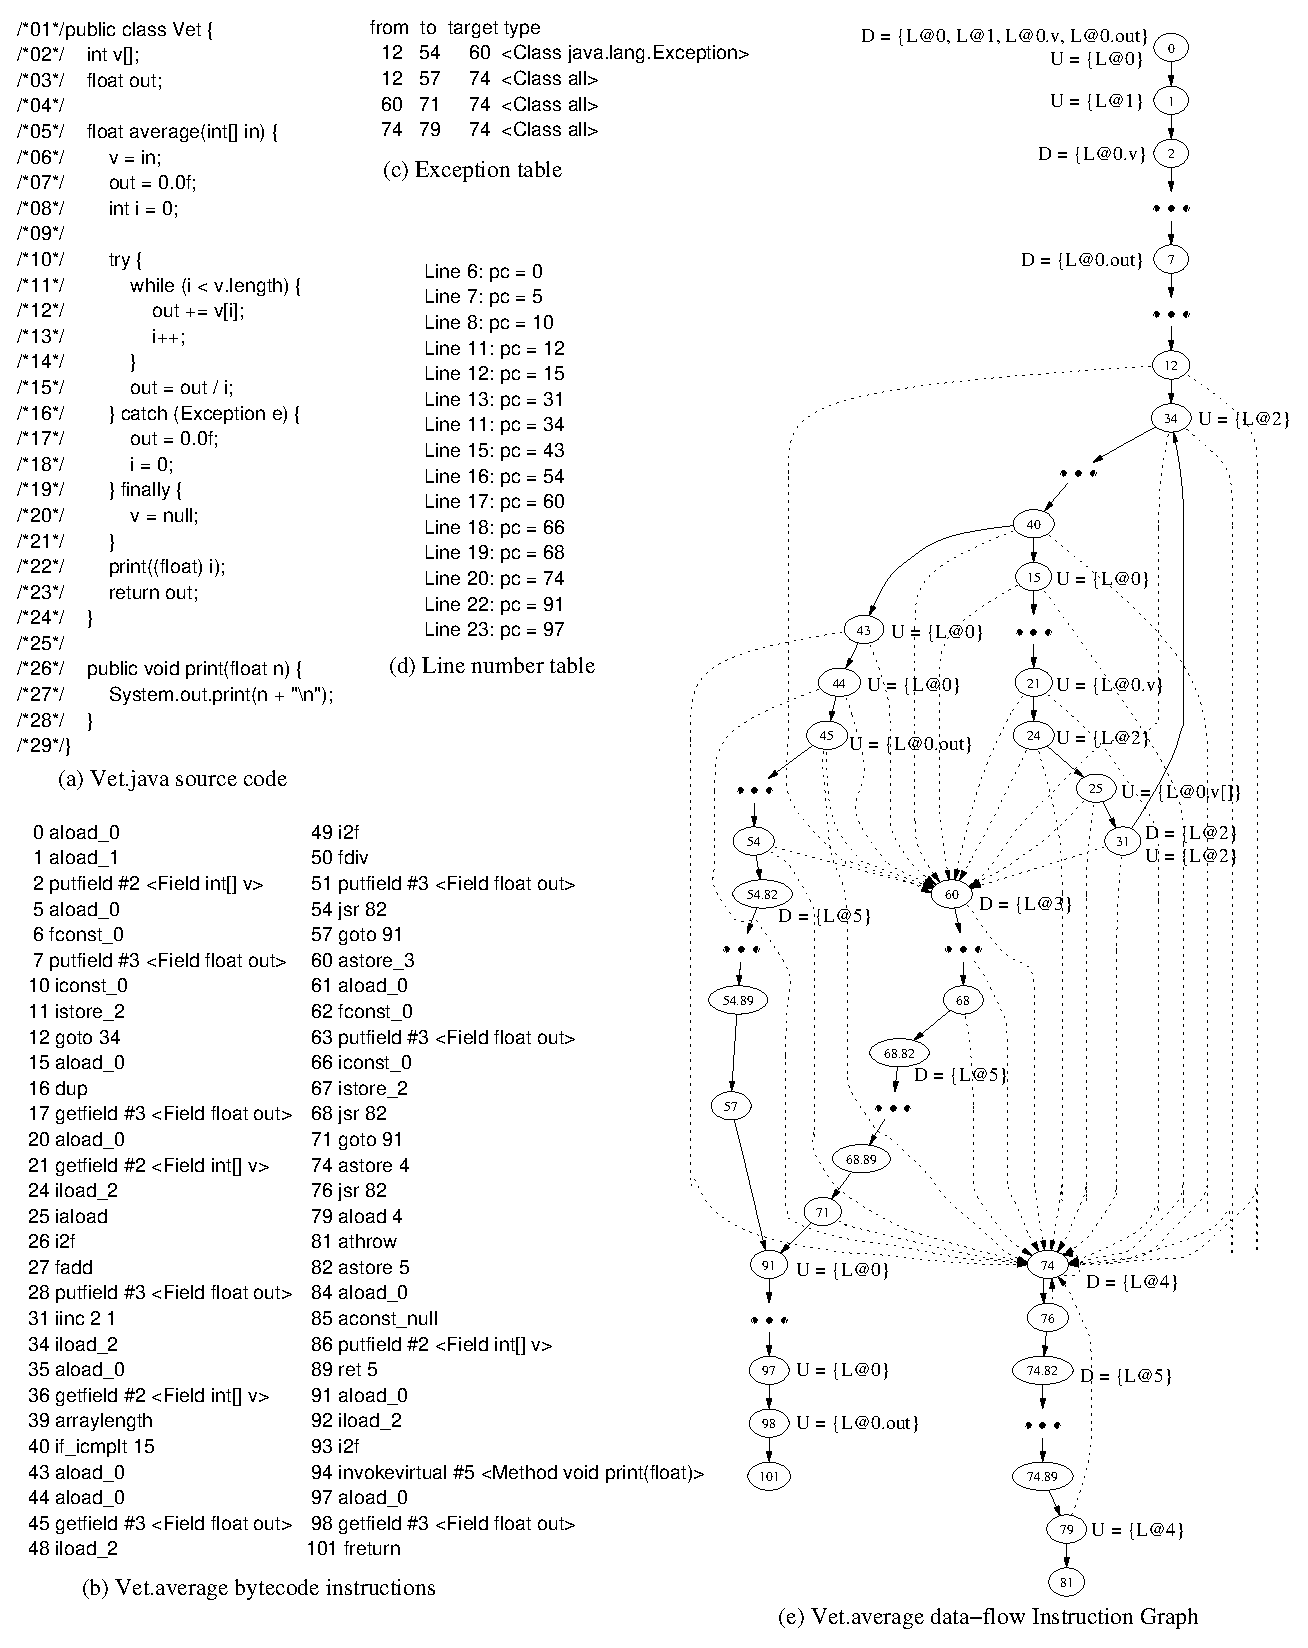
\includegraphics[width=0.9\textwidth]{fig/Vet.average.all.eps}
\caption{Illustration of the data-flow \IG.}\label{fig:average}
\end{center}
\end{figure}


The bytecode instructions can be related to source code lines
because the class file stores information that maps each bytecode
instruction to the source line it appears on. Thus, if the source
code is available, analysis applied on the bytecode level can be
mapped back to the source code level. The line number table,
illustrated in Figure~\ref{fig:average}(d), gives the
correspondence between source line number and bytecode program
counter. For example, the statement at the source line number 06
corresponds to the bytecode instructions from \pc 0 to \pc 2. The
bytecode instructions from \pc 5 to 7 correspond to the statement
at source line 07, and so on.

To construct \IG, the bytecode of a given method is read and an
interpreter is responsible for analyzing the semantics of each
instruction, identifying the set of nodes and edges of the \IG.
First, a node is created in the \IG for each bytecode instruction,
and such nodes are connected by primary edges, considering the
existence of control transfer between each instruction, and by
secondary edges, considering the exception table. From the
complete set of bytecode instructions presented in
Table~\ref{tab:classes} (Section~\ref{sec:data-info}), the
instructions in bold from Class~0 and Class~1 (first and second
rows) are related with the control-flow aspect of Java bytecode.
Figure~\ref{fig:average}(e) illustrates the resulting \IG of the
method presented in Figure~\ref{fig:average}(b). The \IG nodes are
numbered according to the \pc number of the bytecode instruction
it represents. Section~\ref{sec:data-info} describes how to
identify the set \var{D$_i$} of defined variables and the set
\var{U$_i$} of used variables associated to each node of \IG.
Observe that at bytecode level it is not possible to distinguish
between a \emph{p-use} and a \emph{c-use}. Later, in the
computation of the data-flow criteria, nodes with more than one
outgoing edge will have the uses associated to such edges, as if
they were \emph{p-uses}.

Since in the \IG each bytecode instruction corresponds to a node,
the number of nodes and edges can be very large, even for methods
with a few lines of code. In case of the \IG in
Figure~\ref{fig:average}(e), some nodes are omitted in order to
reduce the size of the \IG and to make it more readable. Ellipsis
(``$\bullet \bullet \bullet$'') are used to represent omitted
nodes.

Primary edges are represented by continuous lines and secondary
edges by dotted lines. Observe that there are a large number of
secondary edges connecting the nodes in the scope of a given
exception-handler to the first node of the handler. For example,
according to the exception table of Figure~\ref{fig:average}(c)
the exception-handler located at \pc 60 is responsible to catch
all exceptions of \pk{java.lang.Exception} class raised from \pc
12 to \pc 54. So, there are secondary edges connecting all nodes
in this range to node 60. The same applies to the other
exception-handlers.

Special care on building the \IG is required to deal with
subroutine calls inside the method, used, for example, to
implement the \bci{finally} block of Java. Each \bci{jsr}
instruction causes the execution of an intra-method piece of code
(subroutine). After the subroutine has been executed, the
execution is resumed at a different point in the program,
depending on which \bci{jsr} caused the execution of the
subroutine. In our example, there are three \bci{jsr} instructions
located at \pc 54, 68, and 76, all of them representing a branch
to \pc 82, that is the first instruction of the \bci{finally}
block. Such a finally block goes from \pc 82 to \pc 89. Observe
that at \pc 89 there is a \bci{ret} instruction which returns the
execution to \pc 57, 71 or 79, depending on which \bci{jsr}
instruction invoked the subroutine. To avoid any misinterpretation
about which \bci{jsr} instruction causes the invocation of the
\bci{finally} block, and at which instruction the execution is
resumed, the set of nodes that corresponds to the \bci{finally}
block is replicated for each \bci{jsr} instruction, and different
labels are used to identify the replicated nodes. In our example,
nodes 82 to 89 are replicated three times and the labels of such
nodes are preceded by ``54.'', ``68.'', and ``76.'', as can be
observed in Figure~\ref{fig:average}(e).
Figure~\ref{fig-single-finally} illustrates the problem if the
nodes that compose a \bci{finally} block are not replicated.
Observe that since node 82 has three incoming edges and node 89
three outgoing edges this can lead to the false impression that
from any incoming edge there are three outgoing edges while, in
the reality, only one exists. By replicating the nodes in the
subroutine we avoid such a problem, as illustrated in
Figure~\ref{fig-multiple-finally}.

% This is part of the Jabuti 1.0 Manual.
% Copyright 2003 (c) Auri Marcelo Rizzo Vicenzi, Marcio Eduardo Delamaro,
% Jose Carlos Maldonado.
% See the file FDL.TXT for copying conditions.

\begin{figure}[!ht]
\begin{center}
\subfigure[]{\label{fig-single-finally}\includegraphics[scale=0.30]{fig/single-finally.eps}}\qquad\qquad\qquad
\subfigure[]{\label{fig-multiple-finally}\includegraphics[scale=0.30]{fig/multiple-finally.eps}}
\caption{Different approaches to deal with \bci{finally} block:
(a) Single Finally Node (b) Multiple Finally
Nodes.}\label{fig-finally}
\end{center}
\end{figure}


\subsubsection{Augmenting the \IG: Data-Flow
\IG}\label{sec:data-info}

The first thing required to augment the \IG with data-flow
information is to precisely define the underlying data-flow model
which indicates what kinds of bytecode instructions lead to
variable definition/use and also how to consider reference and
array variables. By analyzing the set of bytecode instructions
obtained from~\cite{Lindholm99JVMS} we classify such instructions
in eleven different classes, according to their relation with the
data-flow at bytecode level. Table~\ref{tab:classes} illustrates
these classes of instructions.

% This is part of the Jabuti 1.0 Manual.
% Copyright 2003 (c) Auri Marcelo Rizzo Vicenzi, Marcio Eduardo Delamaro,
% Jose Carlos Maldonado.
% See the file FDL.TXT for copying conditions.

\begin{table}[!ht]
\caption{Different classes of bytecode
instruction.}\label{tab:classes}
\begin{center}\scriptsize
\begin{tabular}{|c|p{0.4\textwidth}|p{0.4\textwidth}|}\hline
\textbf{Class}&\textbf{Bytecode Instructions}&\textbf{Data-Flow Implication}\\\hline
0   & \setbci{\ctrl{athrow}, \ctrl{goto}, \ctrl{goto\_w},
    \ctrl{if\_acmpeq}, \ctrl{if\_acmpne}, \ctrl{if\_icmpeq}, \ctrl{if\_icmpge},
    \ctrl{if\_icmpgt}, \ctrl{if\_icmple}, \ctrl{if\_icmplt}, \ctrl{if\_icmpne},
    \ctrl{ifeq}, \ctrl{ifge}, \ctrl{ifgt}, \ctrl{ifle}, \ctrl{iflt}, \ctrl{ifne},
    \ctrl{ifnonnull}, \ctrl{ifnull}, \ctrl{lookupswitch}, \ctrl{tableswitch},
    \ctrl{areturn}, \ctrl{dreturn}, \ctrl{freturn}, \ctrl{ireturn}, \ctrl{lreturn}, \ctrl{return},
    \ctrl{ret},
    monitorenter, monitorexit, pop, pop2,
    breakpoint, impdep1, impdep2, nop,
    checkcast,
    wide, swap} &
    Instructions in this class have \textbf{no implication} for the flow of data.\\\hline
1   &  \setbci{\ctrl{invokeinterface}, \ctrl{invokespecial}, \ctrl{invokestatic}, \ctrl{invokevirtual},
    \ctrl{jsr}, \ctrl{jsr\_w},
    dadd, ddiv, dmul, dneg, drem, dsub, fadd, fdiv, fmul, fneg, frem, fsub,
    iadd, iand, idiv, imul, ineg, ior, irem, ishl, ishr, isub, iushr, ixor,
    ladd, land, ldiv, lmul, lneg, lor, lrem, lshl, lshr, lsub, lushr,
    lxor,
    arraylength, instanceof,
    aconst\_null, bipush, dconst, fconst, iconst, lconst, sipush,
    ldc, ldc\_w, ldc2\_w,
    d2f, d2i, d2l, f2d, f2i, f2l, i2b, i2c, i2d, i2f, i2l, i2s, l2d, l2f,
    l2i,
    new, multianewarray, anewarray, newarray,
    dcmpg, dcmpl, fcmpg, fcmpl, lcmp}
    &
    Instructions in this class have \textbf{no implication} for the flow of data.
    In addition, they leave an unknown element at the top of the operand stack.
    Accesses to such element will not characterize any use or definition. For example,
    instruction \bci{new} pushes an object reference onto the stack. Further use
    of such reference as a field access is not regarded as a definition or use.\\\hline
2   & \setbci{aaload, baload, caload, daload, faload,
    iaload, laload, saload}
    & Loads an array element to the top of the operand stacks and
    indicating the \textbf{use} of the array.\\\hline
3   & \setbci{aastore, bastore, castore, dastore,
    fastore, iastore, lastore, sastore}
    & Stores the value on the top of the operand stack
    into an array element, indicating the \textbf{definition} of the array.\\\hline
4   & \setbci{putfield}
    & Stores the value on the top of the operand stack into an
    instance field, indicating the \textbf{definition} of such an instance field.\\\hline
5   & \setbci{putstatic}
    & Stores the value on the top of the operand stack into a
    class field, indicating the \textbf{definition} of such a class field.\\\hline
6   & \setbci{dup, dup2, dup\_x1, dup\_x2, dup2\_x1, dup2\_x2}
    & Duplicates the value onto the top of the operand stack and
    has \textbf{no implication} for the flow of data.\\\hline
7   & \setbci{aload, dload, fload, iload, lload}
    & Loads the value of a given local variable onto the top
    of the operand stack, indicating a \textbf{use} of such a local variable.\\\hline
8   & \setbci{astore, dstore, fstore, istore, lstore}
    & Stores the value on
    the top of the operand stack into a local variable,
    indicating a \textbf{definition} of such a variable.\\\hline
9   & \setbci{getfield}
    & Loads an instance field onto the top of the operand stack,
    indicating a \textbf{use} of such an instance field.\\\hline
10  & \setbci{getstatic}
    & Loads a class field onto the top of the operand stack,
    indicating a \textbf{use} of such a class field.\\\hline
11  & \setbci{iinc}
    & Increments the value of a given local variable,
    indicating a \textbf{use} and a
    \textbf{definition} of such a local variable.\\\hline
\end{tabular}
\end{center}
\end{table}


The division into such classes was based on the kind of
definitions and uses that we would like to identify. In Java and
Java bytecode, the variables can be classified in two types: basic
or reference types. Fields of a class can be of basic or reference
type and are classified as instance or class fields, depending on
whether they are unique to each object of the class or unique to
the entire class (static fields), respectively. Local variables
declared inside a method can also be of basic or reference type.
An aggregated variable (array) is of reference type. To deal with
aggregated variables we are following the approach proposed by
Horgan and London~\cite{Horgan91DFCC}, which considers an
aggregated variable as a unique storage location such that when a
definition (use) of any element of the aggregated variable occurs,
what is considered to be defined (used) is the aggregated variable
and not a particular element. Moreover, in their data-flow model,
a definition of a given variable blocks previous definitions of
the same variable. So, in our data-flow model the following
guidelines apply to identify definitions and uses of variables:

\begin{enumerate}
    \item Aggregated variables are considered as a unique
    storage location and the definition/use of any element of
    the aggregated variable \var{a[]} is considered to be a
    definition/use of \var{a[]}. So, in the statement
    ``\var{a[i] = a[j] + 1}'' there is a definition and a use of
    the aggregated variable \var{a[]}.

    \item If an aggregate variable \var{a[][]} is defined, an access to
    its elements is considered a definition or use of \var{a[][]}. Then,
    in the statement ``\var{a[0][0] = 10}'' there exists a definition
    of \var{a[][]} and in the statement ``\var{a[0] = new
    int[10]}'' there is a definition of \var{a[]}.

    \item Every time an instance field (or an array element)
    is used (defined) there is a use of the reference variable used to access the field
    and a use (definition) of the field itself. Considering
    \var{ref\_1} and \var{ref\_2} as reference variables of a class
    \var{C} which contains two instance fields \var{x} and \var{y} of
    type \var{int}, in the statement ``\var{ref\_1.x = ref\_2.y}''
    there are uses of the reference variables \var{ref\_1} and \var{ref\_2},
    a use of the instance field \var{ref\_2.y}, and a definition of the
    instance field \var{ref\_1.x}. Since instance fields are valid in
    the entire scope of a given class, each instance field
    used in the context of a given method is considered
    to have a definition in the first node of the \IG.

    \item Class fields (static fields) can be considered as global variables
     and do not require a reference variable to be
     accessed. Considering a class \var{C} with
     a static fields \var{w} and \var{z}, in the statement
     ``\var{C.z = C.w + y}'' there are a use of \var{C.w} and a definition of
     \var{C.z}. Even if a static field is accessed using a
     reference variable \var{ref\_1} of class \var{C}, such that
     ``\var{ref\_1.w = 10}'', at bytecode level, such a reference is
     converted to the class name and there is no use of the
     reference variable in this statement. Since
     static fields are in the entire scope of a given class,
     each static field used in the context of a given method is
     considered to have a definition in the first node of the \IG.

    \item A method invocation such as \var{ref\_1.foo(e\_1, e\_2, $\ldots$, e\_n)} indicates
    a use of the reference variable, \var{ref\_1}. The rules for
    definition and use identification inside expressions \var{\mbox{e\_1, e\_2, $\ldots$,
    e\_n}} are the same as described on items 1 to 4.

    \item For instance methods, a definition of \bci{this} is assigned to the
    first node of the \IG, and also the definition of each local variable
    corresponding to the formal parameters of such a method, if any.
    For class methods, only the local variables corresponding to the parameters
    are considered, no instance is required to invoke such a method.
\end{enumerate}

Based on these guidelines and on the different classes of bytecode
instructions, the \IG of a given method is traversed and to each
node of such a graph a set \var{D$_i$} of defined variables, and a
set \var{U$_i$} of used variables are assigned. Before explaining
how these two sets are created, it is important to know how these
different kinds of variables are treated at the bytecode level.
Method parameters and variables declared inside the method are
treated as local variables and are bound to the JVM local variable
table as follows: if it is an instance method, local variable
zero, referenced here as \var{L@0}, is bound to the reference to
the current object (\var{this}), \ie, the object that caused the
method invocation. The formal parameters, if any, are bound to the
local variable one (\var{L@1}), two (\var{L@2}), and so on,
depending on the type and on the number of parameters. Finally,
the variables declared inside the method are bound to the
remaining local variables, also depending on the type and the
number of declared variables. For example, considering the source
code of the method \pk{Vet.average}, it can be observed that it is
an instance method which accepts one parameter \var{in} and
declares one local variable \var{i}. \var{L@0} corresponds to
reference to the current object. The formal parameter \var{in}
corresponds to \var{L@1}, and the variable \var{i} corresponds to
\var{L@2}. Three other local variables (\var{L@3}, \var{L@4} and
\var{L@5}) are used by the compiler to implement the
exception-handling mechanism. The method accesses two instance
fields: \var{v}, and \var{out}. Since they are instance fields,
they require a reference to an object of class \pk{Vet} to be
accessed. When no reference is used preceding a field, the
reference to the current object is used. So, \var{v} and \var{out}
are referenced in the bytecode of our example as \var{L@0.v} and
\var{L@0.out}.

To analyze the \IG we implemented a simulator that interprets
bytecode instructions and identifies the type and the source of
data manipulated by each instruction. For example, suppose the
current instruction to be analyzed is \bci{iload\_2}. Such an
instruction, when interpreted by the JVM, pushes onto the top of
the operand stack an integer value stored in \var{L@2}. Our
simulator, instead of pushing an actual value, pushes onto the top
of the stack an indication in the form ``\pk{$<$type$>$ -
$<$data\_source$>$}'' to be used when interpreting the next
bytecode instructions. \pk{$<$type$>$} corresponds to the data
type being manipulated, and \pk{$<$data\_source$>$} to the source
of each data. In this example, instruction \bci{iload\_2} pushes
an indication like ``\pk{int - L@2}'', since \var{L@2} is a data
source of an integer value. Moreover, the load instruction
characterizes a use of \var{L@2} so this variable is inserted in
the set of used variables associated to the current node of the
\IG graph. Different indications are used to represent the
different types of storage places, as described above. In
Figure~\ref{diff-conf}(a), second column, there are different
kinds of indications placed onto the top of the operand stack when
the bytecode instructions in the first column are interpreted. For
a class field (static field) the indication is in the form
``\pk{$<$type$>$ - S@$<$class\_name$>$.$<$field\_name$>$}'', where
\pk{$<$type$>$} is the type of the static field,
\pk{$<$class\_name$>$} is the class name, and
\pk{$<$field\_name$>$} is the name of the static field. A detailed
description of the interpreter and all kinds of indications can be
found in~\cite{Vincenzi03STOO}.

Considering the \IG presented in Figure~\ref{fig:average}(e),
there are the definitions of \var{L@0}, \var{L@1}, \var{L@0.v},
and \var{L@0.out} associated with node~0. Moreover, node~0 also
contains a bytecode instruction of Class~7 (\bci{aload\_0}), which
indicates a use of the loaded local variable, \var{L@0} in this
case. Observe that the bytecode instruction at \pc 0 is one of the
bytecode instructions that corresponds to the statement ``\var{v =
in}'' at source code line 6 of Figure~\ref{fig:average}(a). The
use exists because before initializing such a field, which is
carried out when the instruction located at \pc 2 is executed, the
reference to the current object (\var{L@0}) has to be loaded onto
the top of the operand stack, characterizing the use of such a
local variable.

At node~2, the \bci{putfield} instruction, which belongs to
Class~4, indicates a definition of an instance field, in our case
the instance field \var{v}, referenced as \var{L@0.v}. So, the set
of defined variables at node~2 contains the element \var{L@0.v}.
Finally, the instruction at node~25, \bci{iaload}, belongs to
Class~2 and indicates a use of an element of an array of integers,
so the set of used variables at node~25 contains the element
\var{L@0.v[]}.

One important point to be observed is that, when evaluating a
given instruction, the current top of the operand stacks can have
more that one configuration, depending on the path used to reach
the instruction. Since it is possible to reach a given node
through different instruction sequences, each different possible
stack configuration needs to be evaluated to find the complete set
of defined/used variables in a \IG node. This is performed by
traversing the \IG as many times as necessary, until all possible
combinations have been evaluated, and the complete set of
defined/used variables on each node have been found.

As an example of such a situation, consider the bytecode
instructions illustrated in Figure~\ref{diff-conf}(b). This set of
bytecode instructions corresponds to the piece of source code
shown in Figure~\ref{diff-conf}(a). Figure~\ref{diff-conf}(c)
shows the corresponding data-flow \IG.

Observe that the bytecode instruction at node~30, can be reached
from two different paths: \{16, 17, 20, 23, 24, 28, 30\} or \{16,
17, 20, 27, 28, 30\}. Each of them inserts a different indication
in the top of the operand stack, the first loads \var{L@1} into
the top of the operand stack and the other \var{L@2}. When
executing the bytecode instruction at \pc 30, which stores the
value onto the top of the operand stack in a field of an object,
two possible combinations can occur, the definition of the field
\var{x} of \var{L@1}, or the definition of field \var{x} of
\var{L@2}. Therefore, the complete set of defined variables at \IG
node 30 contains both: \var{L@1.x} and \var{L@2.x}.

\begin{figure}[!ht]
\begin{center}\scriptsize
\begin{tabular}{cc}
\begin{minipage}{0.50\textwidth}
\hspace{1cm}
\begin{tabular}{|l|l|}\hline
\multicolumn{2}{|l|}{\var{r = new Foo();}}\\
\multicolumn{2}{|l|}{\var{s = new Foo();}}\\
\multicolumn{2}{|l|}{\var{(r.x == 0 ? r : s).x = 20;}}\\\hline
\multicolumn{2}{c}{(a) Piece of Java Source Code}\\
\multicolumn{2}{c}{}\\
\multicolumn{2}{c}{}\\\hline \textbf{Bytecode
Instruction}&\textbf{Operand Stack Configuration}\\ \hline \bci{16
aload\_1}        & \begin{minipage}{0.3\textwidth}
                               Foo - L@1\\
                               $\cdots$
                         \end{minipage}\\ \hline
\bci{17 getfield \#4 $<$Field int x$>$}&
\begin{minipage}{0.3\textwidth}
                               int - L@1.x\\
                               $\cdots$
                         \end{minipage}\\ \hline
\bci{20 ifne 27}        & \begin{minipage}{0.3\textwidth}
                               $\cdots$
                         \end{minipage}\\ \hline
\bci{23 aload\_1}        & \begin{minipage}{0.3\textwidth}
                               Foo - L@1\\
                               $\cdots$
                         \end{minipage}\\ \hline
\bci{24 goto 28}        & \begin{minipage}{0.3\textwidth}
                               Foo - L@1\\
                               $\cdots$
                         \end{minipage}\\ \hline
\bci{27 aload\_2}        & \begin{minipage}{0.3\textwidth}
                               Foo - L@2\\
                               $\cdots$
                         \end{minipage}\\ \hline
\bci{28 bipush 20}        & \begin{minipage}{0.3\textwidth}
                               int - DC\\
                               \textbf{Foo - L@1 or Foo - L@2}\\
                               $\cdots$
                         \end{minipage}\\ \hline
\bci{30 putfield \#4 $<$Field int x$>$}&
\begin{minipage}{0.3\textwidth}
                               \textbf{int - L@1.x or int - L@2.x}\\
                               $\cdots$
                         \end{minipage}\\ \hline
\end{tabular}
\end{minipage}
&
\begin{minipage}{0.50\textwidth}
\hspace{3cm}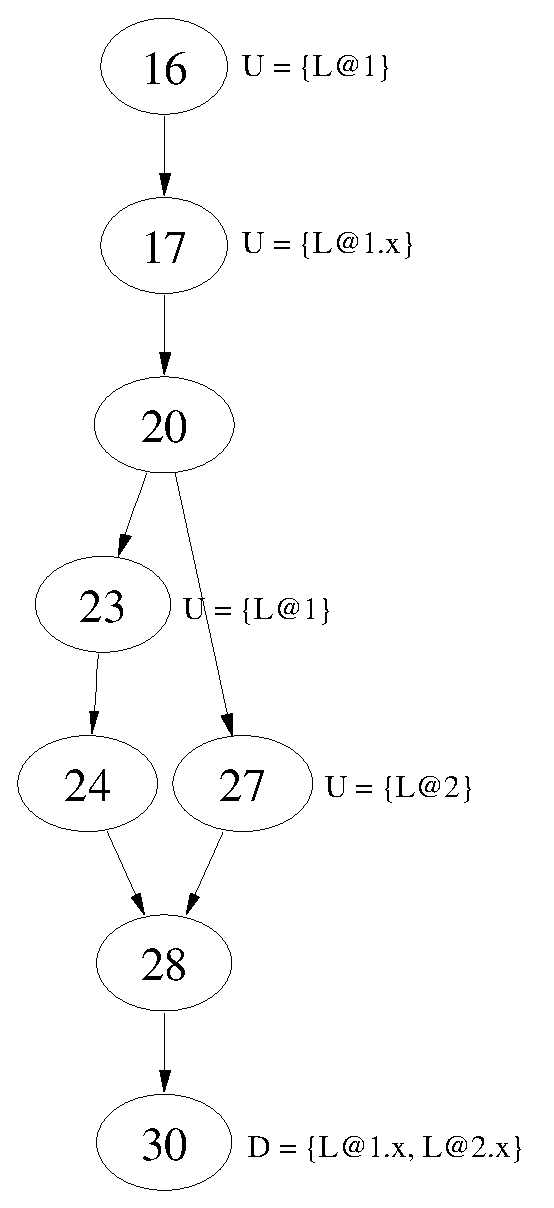
\includegraphics[width=0.38\textwidth]{fig/diff-conf.eps}
\end{minipage}\\
\multicolumn{1}{c}{\hspace{2cm}(b) Bytecode instructions}&
\multicolumn{1}{c}{(c) Corresponding \IG}\\
\end{tabular}
\end{center}
\caption{Different Stack Configurations.}\label{diff-conf}
\end{figure}

Once the complete set of defined and used variables have been
detected, the instruction CFG can be reduced to originate the \BG.
The algorithm used to perform such a reduction is explained in the
next section.

\subsubsection{Constructing Data-Flow Block Graph
(\BG)}\label{sec:bcfg}

The \IG provides a practical way to traverse the set of statements
of a given method to identify the set of variables defined and
used by each statement. However, since a node on \IG is created
for each statement of a given method $m$, the number of nodes and
edges can be very large, especially considering lower level
bytecode instructions. Once all information about each bytecode
instruction has been collected, we use the concept of
\emph{instruction block} to reduce the number of nodes and edges
as much as possible.

An \emph{instruction block} is a set of instructions that are
``normally'' executed in sequence in a program. When the first
instruction of a block is executed, so are the remaining
instructions; branching only occurs to the beginning and from the
end of the block.

A block graph for a given method $m$ is a directed graph
$\mathcal{BG}(m) = (N, E_p, E_s, s, T)$ such that, each node $n
\in N$ represents a instruction block, each edge $(n_i, n_j) \in
E_p$ represents a primary edge (control transfer) between blocks
$n_i$ and $n_j$, each edge $(n_i, n_j) \in E_s$ represents a
secondary edge between blocks $n_i$ and $n_j$, $s$ corresponds to
the start block, and $T$ is the set of termination blocks. For
each block two sets \var{D$_i$} and \var{U$_i$} are assigned. They
contain the sets of defined and used variables in the block,
respectively.

The algorithm used to reduce a data-flow \IG to a data-flow  \BG
is presented in Figure~\ref{fig:algorithm}. In line 14 of the
algorithm, a decision is taken whether the current instruction $x$
being analyzed is the last one in the current block or not. It
will be the last one if at least one of the following conditions
holds:

\begin{itemize}
   \item $x$ is a jump, goto, ret or invoke instruction;
   \item $x$ has more than one primary successor;
   \item the single primary successor of $x$ has more than
         one (primary or secondary) predecessor;
   \item the single primary successor of $x$ has not the
         same set of secondary successors of $x$.
\end{itemize}

% This is part of the Jabuti 1.0 Manual.
% Copyright 2003 (c) Auri Marcelo Rizzo Vicenzi, Marcio Eduardo Delamaro,
% Jose Carlos Maldonado.
% See the file FDL.TXT for copying conditions.

\begin{figure}[!ht]
{\cmdsize
\begin{center}
\begin{tabular}{|l|}\hline\\
\begin{minipage}{5in}
\noindent\# Input: $iG$, the instruction-CFG $GI = \langle NI, EI_p,EI_s, si, TI\rangle$ to be reduced; \\
\# Output: $bG$, the block CFG $bG = \langle N, E_p, E_s, s,
T\rangle$
\\ \ \\
%
01\bigind    s := NewNodeTo(si) \\
02\bigind    foreach $x \in N$ \\
03\bigind    \ind if $x$ has no successor \\
04\bigind    \ind\ind $T := T \cup \{x\}$ \\ \ \\
%
     \# Auxiliary function: NewNodeTo \\
     \# Input: A node $y$ from $iG$ \\
     \# Output: A node from $bG$ where $y$ has been inserted \\ \ \\
%
05\bigind     $ins$ := the instruction in $y$ \\
06\bigind     if the node $y$ has already been visited \\
07\bigind     \ind return the node $w \in N$ that contains $ins$ \\
08\bigind     $CurrentNode :=$ new block node \\
09\bigind     $N := N \cup \{CurrentNode\}$ \\
10\bigind     $x := y$ \\
11\bigind     repeat \\
12\bigind     \ind Include $x$ as part of $CurrentNode$ \\
13\bigind     \ind Mark $x$ as visited \\
14\bigind     \ind if $x$ should terminated the current block \\ % aqui � linha xx
15\bigind     \ind\ind foreach $v$ such that $(x,v) \in EI_p$ \\
16\bigind     \ind\ind\ind $E_p := E_p \cup \{(CurrentNode, NewNodeTo(v))\}$ \\
17\bigind     \ind\ind foreach $v$ such that $(x,v) \in EI_s$ \\
18\bigind     \ind\ind\ind $E_s := E_s \cup \{(CurrentNode, NewNodeTo(v))\}$ \\
19\bigind     \ind\ind $x := null$ \\
20\bigind     \ind else \\
21\bigind     \ind\ind if there exists a $v$ such that $(x,v) \in EI_p$ \\
22\bigind     \ind\ind\ind $x := v$ \\
23\bigind     \ind\ind else \\
24\bigind     \ind\ind\ind $x := null$ \\
25\bigind     while $x \neq null$ \\
26\bigind     return $CurrentNode$ \\
\end{minipage}\\\hline
\end{tabular}
\end{center}
}
\caption{Algorithm to generate the CFG from bytecode.}\label{fig:algorithm}
\end{figure}


Zhao~\cite{Zhao99ACFJ} proposes a different approach to construct
the CFG of a given method. According to Zhao's approach, if an
exception-handler is present, a new node is also created for any
instruction that may throw an exception explicitly (instruction
\bci{athrow}) or implicitly (other 42 instructions), which can
increase significantly the number of nodes in the CFG. Moreover,
to correctly implement the approach to generate the CFG as
proposed by Zhao~\cite{Zhao99ACFJ} it is necessary to check the
subclasses of each exception that may be raised and to identify if
there is any exception-handler that can catch this particular
exception. In our implementation we decide to use a more pragmatic
approach to construct the \BG, expecting to obtain simpler and
more readable graphs.

As mentioned earlier, two points that should be highlighted are:
first, when we have subroutine calls, the set of statement blocks
representing the subroutine is expanded for every call, \ie, the
statements of a given subroutine may appear more than once in the
\BG within different nodes, once for each subroutine call.

Second, observe that since the set of bytecode instructions on
each statement block might not throw all kind of handled
exceptions, our \BG may have ``false'' (or spurious) secondary
edges. Moreover, the execution of a given block can be interrupted
in any place, when an exception is thrown, so in the presence of
exceptions the block may not have the ``atomicity'' characteristic
mentioned above. On the other hand, this approach simplifies both
the construction of the \BG and also its interpretation, since the
number of nodes is reduced. An alternative approach to construct a
CFG to deal with exception-handling constructions is described by
Sinha and Harrold~\cite{Sinha98APEH} such that no false edges are
generated. Although, the proposed technique considers only
exceptions generated explicitly, \ie, the ones originate by the
\bci{throw} statement~\cite{Sinha98APEH}.

%--------------------------------
%----
%----
%---- There is a good example and figure describing the
%---- exception-handling mechanism in the paper
%---- "Analysis of Programs with Exception-Handling Constructs"
%---- \cite{Sinha98APEH}
%----
%----
%--------------------------------

% This is part of the Jabuti 1.0 Manual.
% Copyright 2003 (c) Auri Marcelo Rizzo Vicenzi, Marcio Eduardo Delamaro,
% Jose Carlos Maldonado.
% See the file FDL.TXT for copying conditions.

\begin{figure}[!ht]
\begin{center}
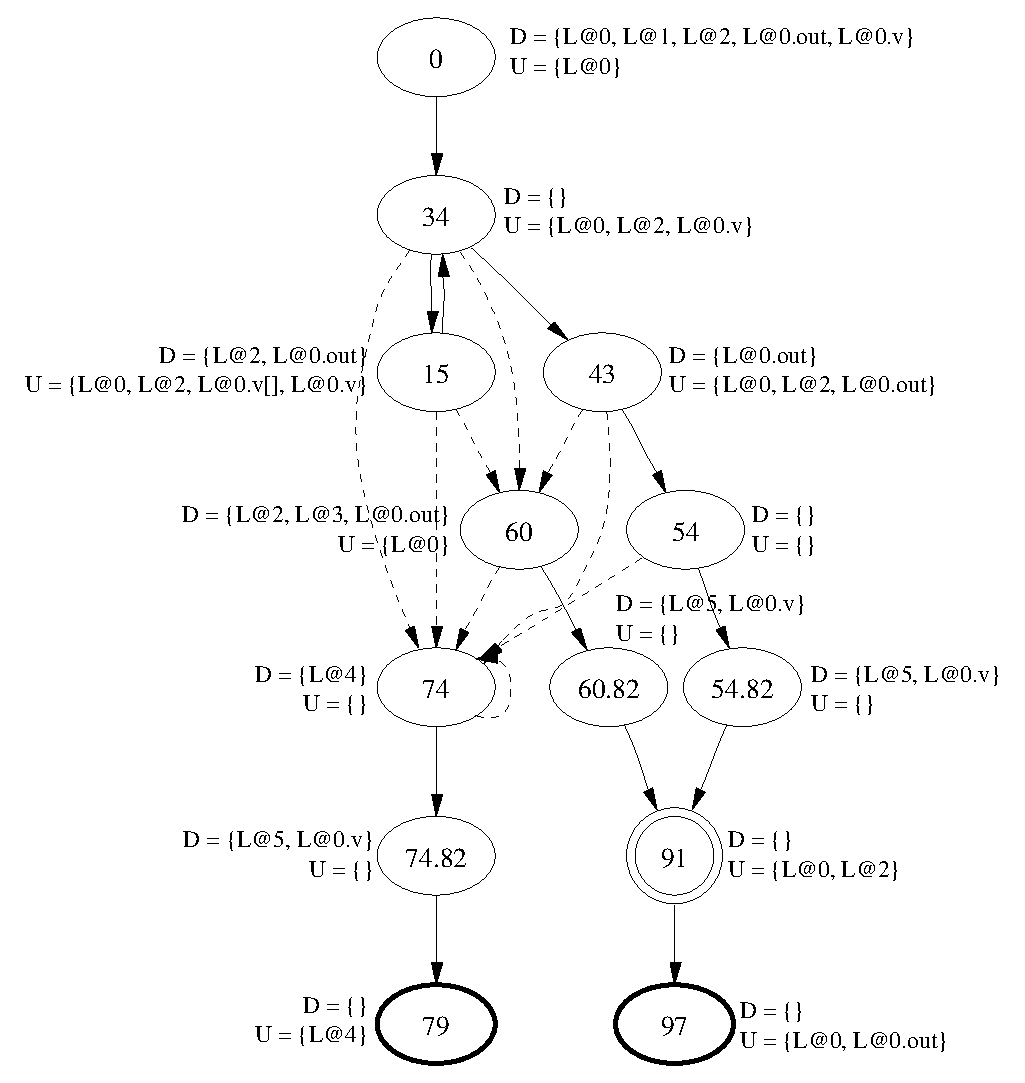
\includegraphics[scale=0.50]{fig/average-bcfg.eps}
\caption{\pk{Vet.average}'s \BG.}\label{fig-average-bcfg}
\end{center}
\end{figure}


After the \BG has been constructed, a simple analysis is carried
out to eliminate unnecessary nodes, \ie, nodes that contain only a
single \bci{goto} instruction. They can be eliminated by directly
connecting its in-coming edges as the in-coming edges of its
successor. Figure~\ref{fig-average-bcfg} illustrated the \BG
obtained by applying the reduction algorithm to the \IG of
Figure~\ref{fig:average}(e). \BG represents the underlying model
used to derive control-flow and data-flow testing requirements.
The label of a given block in \BG is the program counter number of
its first instruction. The labels of the replicated nodes, \ie,
nodes corresponding to a subroutine, are preceded by the label of
the node that invoked the subroutine. Observe that since
instruction node 68 of \IG now composes the block node 60 in \BG,
instructions nodes 68.82 of \IG correspond to block node 60.82 in
\BG. All the other replicated instruction nodes that correspond to
the finally block, \ie, instruction nodes 84, 85, 86 and 89 in
\IG, are part of the block nodes $xx$.82 in \BG.

On constructing the \BG we also have two different types of edges
to represent primary edges (continuous line) and secondary edges
(dashed lines). Moreover, we make a distinction among three
different types of nodes in \BG: termination nodes represented by
bold line circles (as blocks 79 and 97 in
Figure~\ref{fig-average-bcfg}); call nodes represented by double
line circles (as block 91 in Figure~\ref{fig-average-bcfg}); and
regular nodes represented by single line circles (as all other
nodes in Figure~\ref{fig-average-bcfg}). The call nodes are being
distinguished from the others because we intend to extend our
analysis to inter-method level; thus, call nodes are useful for
constructing the inter-method control-flow and data-flow graphs.
Def-use information is trivially computed for each \BG node by the
union of the definition (use) sets of each \IG node included in
the \BG node.

Once the \BG has been obtained, different testing criteria can be
applied to derive different testing requirements that can be used
to assess the quality of a given test set or to generate a given
test set. In the next section we describe some of the testing
criteria that we are working on and the set of testing
requirements derived from each one.

\subsection{Intra-method Structural Testing Requirements}\label{sec:criteria}

Java bytecode can be thought of as an assembly-like language from
that control-flow and data-flow information can be collected and
represented as a \BG, as described above. Once collected, such
information for each method, intra-method testing criteria can be
defined and applied. Basically, at method level, as mentioned
in~\cite{Harrold94PDFT}, traditional control-flow and data-flow
testing criteria~\cite{Rapps85SSTD} can be applied, since they are
based on the same underlying representation, \ie, the \BG. Sinha
and Harrold~\cite{Sinha99CTEH} describe a set of data-flow based
testing criteria considering exceptions. Thus we can adopt
coverage criteria for the later~\cite{Rapps85SSTD,Sinha99CTEH}. We
propose to conduct coverage testing on Java programs, including
Java components with respect to six different testing criteria:
four are control-flow-based and two are data-flow-based.

\subsubsection{Control-Flow Testing
Requirements}\label{sec:ctrl-requirements}

The \BG is a representation of a given method in a program.
Control-flow testing criteria can be derived based on such a
program representation to provide a theoretical and systematical
mechanism to select and assess the quality of a given test set. We
are using two well known control-flow testing criteria to derive
testing requirements from the \BG: \emph{all-nodes} and
\emph{all-edges}~\cite{Roper94STES}.

\begin{itemize}
    \item \textbf{all-nodes criterion}: requires that each \BG node has been
    exercised at least once by a test case in the test set. This criterion
    ensures that every statement in the method have been executed
    at least once by a given test case. we decided
    to subdivide such criterion in two non-overlapping testing
    criteria such that the tester can concentrate on different
    aspects of a program at a time:

    \begin{itemize}
        \item \textbf{all-primary-nodes}: requires that each primary
        node has been exercised at least once by a test case in the
        test set. This criterion requires that all statements not related
        with exception-handling mechanism were executed at least once;

        \item \textbf{all-secondary-nodes}: requires that each
        secondary node has been exercised at least once by a test case in the
        test set. This criterion requires that all statements related
        with exception-handling mechanism were executed at least once;
    \end{itemize}


    \item \textbf{all-edges criterion}: requires that each \BG edge
    has been exercised at least once by a test case in the test set.
    This criterion ensures that every possible control transfer in
    the method
    has been executed at least once by a given test case. Since
    in our \BG there are two different types of edges, we decided
    to subdivide such criterion in two non-overlapping testing
    criteria:

    \begin{itemize}
        \item \textbf{all-primary-edges}: requires that each primary
        edge has been exercised at least once by a test case in the
        test set. This criterion requires that all conditional
        expressions were evaluated as true and false at least once;

        \item \textbf{all-secondary-edges}: requires that each
        secondary edge
        has been exercised at least once by a test case
        in the test set. This criterion requires that each
        exception-handler be executed at least once from each node
        where an exception might be raised.
    \end{itemize}
\end{itemize}

To illustrate how such criteria can be applied,
Table~\ref{tab-ctrl-requirements} presents the set of testing
requirements required by each one of them, considering the \BG of
the method \pk{Vet.average} (Figure~\ref{fig-average-bcfg}).

\begin{table}[!ht]
\begin{center}\cmdsize
\caption{Set of control-flow testing requirements for
\pk{Vet.average} \BG.}\label{tab-ctrl-requirements}
\begin{tabular}{|c|c|p{0.6\textwidth}|}
  \hline
  % after \\: \hline or \cline{col1-col2} \cline{col3-col4} ...
  \multicolumn{2}{|c|}{\textbf{Criterion}} & \textbf{Testing Requirements} \\
  \hline
  \multirow{2}{1.5cm}{\centering all-nodes} &
    \multirow{1}{3cm}{\centering all-primary-nodes} & \{0, 15, 34, 43, 54, 54.82, 91, 97\} \\ \cline{2-3}
  & \multirow{1}{3cm}{\centering all-secondary-nodes} & \{60, 60.82, 74, 74.82, 79\} \\
  \hline

  \multirow{4}{1.5cm}{\centering all-edges} & \multirow{2}{3cm}{\centering all-primary-edges} & \{(0,34), (15,34), (34,15), (34,43), (43,54),
                                                         (54,54.82), (54.82,91), (60,60.82),
                                                         (60.82,91), (74,74.82), (74.82,79), (91,97) \} \\
               \cline{2-3}
  & \multirow{2}{3cm}{\centering all-secondary-edges} & \{(15,60), (15,74), (34,60), (34,74), (43,60), (43,74), (54,74),
  (60,74), (74,74)\} \\
  \hline
\end{tabular}
\end{center}
\end{table}

\subsubsection{Complexity Analysis of Control-Flow Testing
Criteria}

\rev{TO BE DONE...}

\subsubsection{Data-Flow Testing
Requirements}\label{sec:data-requirements}

With respect to data-flow testing, we are using the well known
\emph{all-uses} criterion~\cite{Rapps85SSTD} that is composed of
the \emph{all-c-uses} and \emph{all-p-uses} criteria. A precise
definition about these criteria can be found
in~\cite{Rapps85SSTD}. A {\em use} represents the use of a
variable in a statement. If the value of a variable is used for
some computation, it is a {\em c-use} (Computational Use), whereas
if the value is used in a predicate that determines which branch
is to be executed, it is a {\em p-use} (Predicate Use). Let $b_i$
and $b_j$ to be two points in the bytecode where a variable $x$ is
defined and used, respectively. This definition and this use are
referred to as $d_i(x)$ and $u_j(x)$, respectively. The pair
$(d_i(x), u_j(x))$ is a def-use pair if there is a definition
clear path with respect to $x$ from $b_i$ to $b_j$, \ie, $x$ is
not defined at any point other than $b_i$. The pair is also said
feasible if there exists a test case $t$ such that the execution
of the method on $t$ causes such definition clear path from $b_i$
to $b_j$ to be traversed.

For an example of a c-use, consider the \DUG of
Figure~\ref{fig-average-bcfg}. At node 0, the variable definition
set contains the variable \var{L@0.v}, which represents the
instance variable \var{v} in the corresponding source code. At
node 15 there is a use of \var{L@0.v} to compute the sum of its
elements, determining a c-use pair \wrt \var{L@0.v} from node 0 to
node 15 (c-use). On the other hand, at node 15, there is a
definition of \var{L@2} that represents the local variable \var{i}
in the corresponding source code. Such a variable is used in the
predicate located at node 34 to evaluate if the end of \var{v} has
been reached. Thus, there is a p-use pair \wrt \var{L@2} from node
15 to node 34. From the bytecode, it is not possible to
distinguish p-uses and c-uses. In our implementation of all-uses
criterion we assume that a use in a node with more than one
out-going edge is a p-use and associate it with each of those
edges. As with the all-edges criterion, we divided the all-uses
criterion such that two sets of non-overlapping testing
requirements are obtained, to consider the primary and secondary
edges. We named such criteria all-primary-uses and
all-secondary-uses, respectively. The first takes all the def-use
pairs for which there exists a path of primary edges only. The
other def-use pairs are required by the second.

To illustrate how such criteria can be applied,
Table~\ref{tab-data-requirements} presents the set of testing
requirements required by each one of than, considering the \BG of
the method \pk{Vet.average} (Figure~\ref{fig-average-bcfg}).

A test set $T$ may be evaluated against the all-uses criterion
(all-primary-uses/all-secondary-uses) by computing the ratio of
the number of def-use pairs covered to the total of all-uses
(all-primary-uses/all-secondary-uses) requirements. The same
applies to all-nodes and all-edges
(all-primary-edges/all-secondary-edges) criteria. More details
about the testing criteria definition can be found
in~\cite{Vincenzi03STOO}.

\begin{table}[!ht]
\begin{center}\cmdsize
\caption{Set of data-flow testing requirements for
\pk{Vet.average} \BG.}\label{tab-data-requirements}
\begin{tabular}{|c|c|ccc|}
  \hline
  % after \\: \hline or \cline{col1-col2} \cline{col3-col4} ...
  \multicolumn{2}{|c|}{\textbf{Criterion}} & \multicolumn{3}{l|}{\textbf{Testing Requirements}} \\
  \hline
  \multirow{20}{1.5cm}{\centering all-uses} & \multirow{10}{3cm}{\centering all-primary-uses} &
\ass{L@0}{0}{\edg{15}{34}} & \ass{L@0}{0}{\edg{34}{15}} &
\ass{L@0}{0}{\edg{34}{43}} \\ & & \ass{L@0}{0}{\edg{43}{54}} &
\ass{L@0}{0}{\edg{60}{60.82}} & \ass{L@0}{0}{54.82} \\ & &
\ass{L@0}{0}{60.82} & \ass{L@0}{0}{74.82} & \ass{L@0}{0}{91} \\ &
& \ass{L@0}{0}{97} & \ass{L@0.out}{0}{\edg{43}{54}} &
\ass{L@0.out}{15}{\edg{43}{54}} \\ & & \ass{L@0.out}{43}{97} &
\ass{L@0.out}{60}{97} & \ass{L@0.v}{0}{\edg{15}{34}} \\ & &
\ass{L@0.v}{0}{\edg{34}{15}} & \ass{L@0.v}{0}{\edg{34}{43}} &
\ass{L@0.v[]}{0}{\edg{15}{34}} \\ & & \ass{L@2}{0}{\edg{15}{34}} &
\ass{L@2}{0}{\edg{34}{15}} & \ass{L@2}{0}{\edg{34}{43}} \\ & &
\ass{L@2}{0}{\edg{43}{54}} & \ass{L@2}{0}{91} &
\ass{L@2}{15}{\edg{15}{34}} \\ & & \ass{L@2}{15}{\edg{34}{15}} &
\ass{L@2}{15}{\edg{34}{43}} & \ass{L@2}{15}{\edg{43}{54}} \\ & &
\ass{L@2}{15}{91} & \ass{L@2}{60}{91} & \ass{L@4}{74}{79}
\\\cline{2-5}
  & \multirow{11}{3cm}{\centering all-secondary-uses} &
\ass{L@0}{0}{\edg{15}{60}} & \ass{L@0}{0}{\edg{15}{74}} &
\ass{L@0}{0}{\edg{34}{60}} \\ & & \ass{L@0}{0}{\edg{34}{74}} &
\ass{L@0}{0}{\edg{43}{60}} & \ass{L@0}{0}{\edg{43}{74}} \\ & &
\ass{L@0}{0}{\edg{60}{74}} & \ass{L@0.out}{0}{\edg{43}{60}} &
\ass{L@0.out}{0}{\edg{43}{74}} \\ & &
\ass{L@0.out}{15}{\edg{43}{60}} & \ass{L@0.out}{15}{\edg{43}{74}}
& \ass{L@0.out}{43}{\edg{43}{60}} \\ & &
\ass{L@0.out}{43}{\edg{43}{74}} & \ass{L@0.v}{0}{\edg{15}{60}} &
\ass{L@0.v}{0}{\edg{15}{74}} \\ & & \ass{L@0.v}{0}{\edg{34}{60}} &
\ass{L@0.v}{0}{\edg{34}{74}} & \ass{L@0.v[]}{0}{\edg{15}{60}} \\ &
& \ass{L@0.v[]}{0}{\edg{15}{74}} & \ass{L@2}{0}{\edg{15}{60}} &
\ass{L@2}{0}{\edg{15}{74}} \\ & & \ass{L@2}{0}{\edg{34}{60}} &
\ass{L@2}{0}{\edg{34}{74}} & \ass{L@2}{0}{\edg{43}{60}} \\ & &
\ass{L@2}{0}{\edg{43}{74}} & \ass{L@2}{15}{\edg{15}{60}} &
\ass{L@2}{15}{\edg{15}{74}} \\ & & \ass{L@2}{15}{\edg{34}{60}} &
\ass{L@2}{15}{\edg{34}{74}} & \ass{L@2}{15}{\edg{43}{60}} \\ & &
\ass{L@2}{15}{\edg{43}{74}} & & \\\hline
\end{tabular}
\end{center}
\end{table}

\subsubsection{Complexity Analysis of Data-Flow Testing Criteria}

\rev{TO BE DONE...}

\subsection{Dominators and Super-Block Analysis}\label{sec:super-block}

Studies have shown that it is important to generate a test set
with high coverage while testing C programs so that more faults
are likely to be
detected\cite{Piwowarski93CMED,Wong94ETSS,Wong98ETSM}. The same
applies to Java programs without lost of generality. To explain
our approach to increase the coverage as soon as possible \wrt a
given test criterion (all-blocks in our example), consider the \BG
presented in Figure~\ref{fig-average-bcfg}. The main idea is to
assign different weights to each \BG node based on dominator
analysis and ``super block''~\cite{Agrawal94DSBP}. The objective
is to generate a test to cover one of the areas with the highest
weight, if possible, before other areas with a lower weight are
covered so that the maximum coverage can be added in each single
execution. In this way, we provide useful hints on how to generate
efficient test cases to increase, as much as possible with as few
tests as possible, the control-flow (such as block and decision)
and data-flow coverage (such as all-uses) of the programs being
tested.

Basically, a super-block is a subset of nodes with the property
that if any node in a super block is covered then all nodes in
that super block are covered\footnote{Assuming that the
    underlying hardware does not fail and no exception
    is raised during the execution of a test}. Pre- and
post-dominator relationships among nodes are used to identify the
set of super blocks from a given \BG. According
to~\cite{Agrawal94DSBP}, a node $u$ pre-dominates a node $v$
denoted as $u \stackrel{pre}{\rightarrow} v$, if every path from
the entry node to $v$ contains $u$. A node $w$ post-dominates a
node $v$ denoted as $u \stackrel{post}{\rightarrow} v$, if every
path from $v$ to the exit node contains $w$. For example, in
Figure~\ref{fig-average-bcfg}, nodes 0 and 34 pre-dominate node 74
and nodes 74.82 and 79 post-dominate it. Pre- and post-dominator
relationships can be expressed in the form of pre- and post
dominator trees, respectively. $u \stackrel{pre}{\rightarrow} v$
\emph{iff} there is a path from $u$ to $v$ in the predominator
tree. Similarly, $w \stackrel{post}{\rightarrow} v$ \emph{iff}
there is a path from $w$ to $v$ in the post-dominator tree.
Figures~\ref{fig-pre-dominator} and~\ref{fig-post-dominator} show
the pre- and post-dominator trees of the \BG in
Figure~\ref{fig-average-bcfg}.

The dominator relationship amongst \BG's nodes is represented by a
``basic block dominator graph'' that corresponds to the union of
the pre- and post-dominator trees. Figure~\ref{fig-merged-tree}
shows the basic block dominator graph of the \BG in
Figure~\ref{fig-average-bcfg}.

From the basic block dominator graph, strongly connected
components (super blocks) are identified and the corresponding
super block dominator graph is obtained. A strongly connected
component has a property that every node in the component
dominates all other nodes in that component. For example, nodes
\{74, 74.82, 79\} compose a strongly connected component.

Figure~\ref{fig-super-block} represents the super block dominator
tree of the \BG in Figure~\ref{fig-average-bcfg}. From this
representation it is possible to calculate the weight of each \BG
node. Basically, the weight of a given node is the number of nodes
that have not been covered but will be if that block is covered.
In Figure~\ref{fig-super-block-uncovered}, the initial weight of
each super block is show on the bottom of each node.

For example, to arrive at node 54.82 in
Figure~\ref{fig-average-bcfg} requires the execution also to go
through nodes 0, 34, 43, and 54. After arriving in node 54.82,
nodes 91 and 97 will also be executed. This implies node 54.82 is
dominated by nodes 0, 34, 43, 54, 91 and 97. It also means nodes
0, 34, 43, 54, 91 and 97 will be covered (if they haven't been) by
a test execution if that execution covers node 54.82. Assuming
none of the blocks is covered so far, we say that node 54.82 has a
weight of at least 7 because covering it will increase the
coverage by at least seven nodes. Using the same approach, node 15
has a weight of 3 since its coverage only guarantees an increase
of coverage by at least three nodes. A very important note is that
while assigning the weight to a given node, we use a conservative
approach by counting only the additional nodes that will
definitely be covered because of the coverage of this given node.
This is why we use the phrase ``at least'' in the above
statements. Of course, covering a node of a weight 7 (like node
54.82 in our example) may end up covering more than seven blocks
(por ex., the execution can go through nodes 0, 34, 15, 34, 43, 54
before it reaches node 54.82 and continues though nodes 91 and
97). Nevertheless, the additional nodes (node 15 in our example)
are not guaranteed to be covered.

% This is part of the Jabuti 1.0 Manual.
% Copyright 2003 (c) Auri Marcelo Rizzo Vicenzi, Marcio Eduardo Delamaro,
% Jose Carlos Maldonado.
% See the file FDL.TXT for copying conditions.

\begin{figure}[!ht]
\begin{center}
\subfigure[Pre-Dominator
Tree]{\label{fig-pre-dominator}\includegraphics[scale=0.50]{fig/average-dominator-tree.eps}}\qquad
\subfigure[Post-dominator
Tree]{\label{fig-post-dominator}\includegraphics[scale=0.50]{fig/average-idominator-tree.eps}}

\subfigure[Basic Block Dominator
Tree]{\label{fig-merged-tree}\includegraphics[scale=0.50]{fig/average-merged-tree.eps}}\qquad
\subfigure[Super Block Dominator
Tree]{\label{fig-super-block}\includegraphics[scale=0.50]{fig/average-super-block.eps}}
\caption{Control-Flow Dependence Analysis.}\label{fig-super}
\end{center}
\end{figure}


% This is part of the Jabuti 1.0 Manual.
% Copyright 2003 (c) Auri Marcelo Rizzo Vicenzi, Marcio Eduardo Delamaro,
% Jose Carlos Maldonado.
% See the file FDL.TXT for copying conditions.

\begin{figure}[!ht]
\begin{center}
\subfigure[]{\label{fig-super-block-uncovered}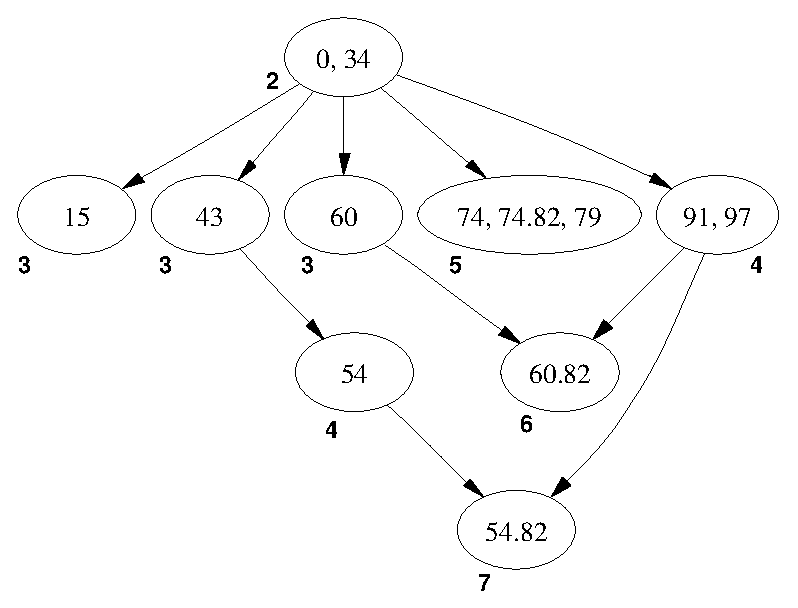
\includegraphics[scale=0.45]{fig/super-block-uncovered.eps}}\qquad
\subfigure[]{\label{fig-super-block-covered}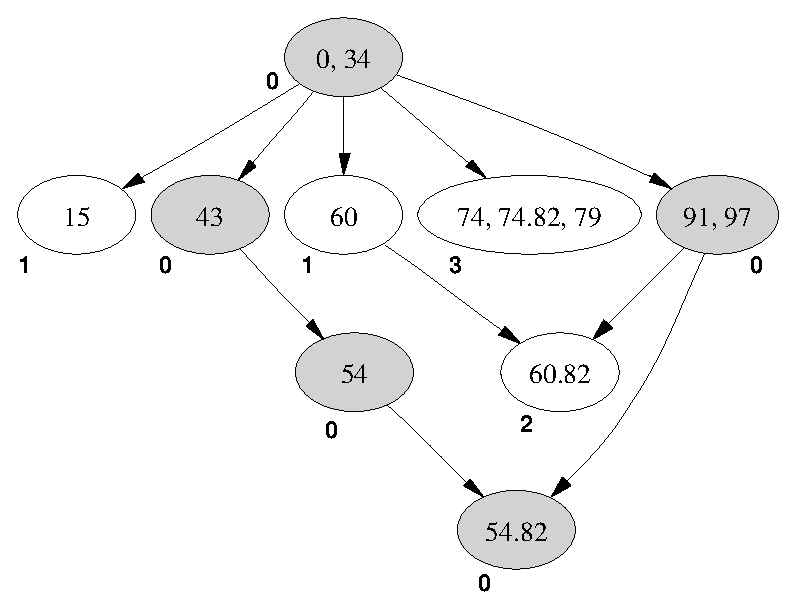
\includegraphics[scale=0.45]{fig/super-block-covered.eps}}
\caption{Super block dominator graph with weights: (a) before any
test case execution, and (b) after the execution of one test
case.}\label{fig-weight}
\end{center}
\end{figure}


Since node 54.82 has a higher weight than node 15, we say that
node 54.82 has a higher priority to be covered than node 15 (\ie,
tests that cover node 54.82 have a higher priority to be executed
than tests that only cover node 15)\footnote{Observe that,
        we are using the term high priority only considering the
        coverage that will be obtained. The tester, based on his
        experience may desire to cover first a node with a lower weight
        but that has a higher complexity in terms of implementation, \ie,
        depending on the criticality of a given part of the code, or based on
        another assumption, the tester can choose to cover a different
        node first and then, by recomputing the weight, to use the weight
        information to increase the coverage faster.
} so that the maximum node coverage can be added in each single
execution. In this way, the node coverage can be increased as much
as possible with as few tests as possible.

After executing certain tests the weights of nodes that are not
covered by these tests may change. For example, after the
execution of a test (say $t_1$) that covers node 54.82 (which also
guarantees the coverage of node 0, 34, 43, 54, 91 and 97), the
execution of another test (say $t_2$) to cover node 15 will
increase the coverage by only one node (namely, node 15 itself).
This is because nodes 0 and 34 have already been covered by test
$t_1$ and the execution of other tests (such as $t_2$) will not
change this fact. Under this scenario, after $t_1$ has been
executed, node 15 will have weight one. This implies that after a
test ($t_1$ in our case) is executed to cover node 54.82, the
priority, in terms of increasing the coverage, of executing
another test ($t_2$ in our case) to cover node 15 may be reduced.

This procedure is applied recursively after the execution of each
test to recompute the weight of each node that has not been
covered by the current tests, as well as the priority of tests to
be executed for covering such nodes. The objective is to continue
this recursive procedure until all the blocks, if possible, are
covered by at least one test (\ie, achieve 100\% node coverage) or
the execution will stop after a predefined time-out been reached.
In the latter case, although tests so executed might not give
100\% node coverage, they still provide as high a block coverage
as possible. \rev{In the reality, as mentioned
in~\cite{Agrawal94DSBP}, the tester only needs to create test
cases that covers one node of each leaf node in the super block
dominator graph to cover all the other nodes.}

\subsection{Program Slicing}\label{sec:slicing}

Computer programmers break apart large programs into smaller
coherent pieces. Each of these pieces: functions, subroutines,
modules, or abstract datatypes, is usually a contiguous piece of
program text. Programmers also routinely break programs into one
kind of coherent piece which is not contiguous. When debugging
unfamiliar programs programmers use program pieces called slices
which are sets of statements related by their flow of control or
data. The statements in a slice are not necessarily textually
contiguous, but may be scattered through a
program~\cite{Weiser82PUSW}. A program slice consists of the parts
of a program that (potentially) affect the values computed at some
point of interest. Such a point of interest is referred to as a
slicing criterion, and is typically specified by a location in the
program in combination with a subset of the program's variables
and/or statements. The task of computing program slices is called
program slicing. The original definition of program slicing was
proposed by Weiser in 1979~\cite{Weiser79PSFP,Weiser84PSLI}.
Today, a lot of slightly different notions of program slices can
be found in the literature, as well as a number of criteria to
compute them~\cite{Tip95SPST}. An important distinction exists
between a static and a dynamic slice. Static slices are computed
without making assumptions regarding a program's input, whereas
the computation of dynamic slices relies on a the execution trace
information of specific test case.

Program slicing is a broadly applicable program analysis technique
that can be used to perform different software engineering
activities, such as: program understanding, debugging, testing,
parallelization, re-engineering, maintenance, and
others~\cite{Gammatech00DGPS}. In the context of \toolname, the
three most important activities are program understanding,
debugging and testing.

\textbf{Program understanding} uses program slicing to help
engineers to understand code. For example, a backward slice from a
point in the program identifies all parts of the code that
contribute to that point. A forward slice identifies all parts of
the code that can be affected by the modification to the code at
the slice point.

\textbf{Testing and Regression Testing} also uses slicing. For
example, suppose a proposed program modification only changes the
value of variable $v$ at program point $p$. If the forward slice
with respect to $v$ and $p$ is disjoint from the coverage of
regression test $t$, then test $t$ does not have to be rerun.
Suppose a coverage tool reveals that a use of variable $v$ at
program point $p$ has not been tested. What input data is required
in order to cover $p$? The answer lies in the backward slice of
$v$ with respect to $p$.

In Section~\ref{sec:slice} it is described the characteristics
\toolname's slicing tool and how to use it to smart debugging and
fault localization.

\subsection{Complexity Metrics}\label{sec:bk-metrics}

Complexity metrics are very useful to several software engineering
tasks. Their main objective is to provide different kinds of
measure of a project/program such that further projects can use
the historical database to better estimate time, cost and
complexity of new projects. There are different kinds of
complexity metrics. For example, Lorenz e Kidd~\cite{Lorenz94OOSM}
defined a set of design metrics to evaluate static characteristics
of an OO software project. The proposed set of metrics is divided
into three groups: 1) \textbf{Class Size Metrics} to quantify
individual classes; 2) \textbf{Class Inheritance Metrics} to
evaluate the quality of using inheritance; and 3) \textbf{Class
Internal Metrics} to evaluate general characteristics of a class.

Another well-known set of metrics, proposer by Chidamber and
Kemerer~\cite{Chidamber94MSOO}, is composed by six design metrics
six design metrics developed to evaluate the complexity of a given
class.

Utsonomia~\cite{Utsonomia02EAMS} have studied and adapted both
sets of design metrics for Java bytecode. \toolname implements
such adapted metrics to allow a tester to collect static metrics
information for the classes under testing.

Another benefit of complexity metrics is that the collected
information can be used to establish incremental testing
strategies by prioritizing the test of certain classes, reducing
the cost and improving the quality of the testing activity. For
instance, \toolname prioritizes testing requirements based on
coverage information. By using complexity metrics, the class's
inheritance, size, and complexity can be combined with coverage
information, providing additional hints to reduce the cost of test
case generation.

In Section~\ref{sec:metrics} it is described how to use \toolname
to collect static information about the classes under testing,
considering the set of complexity metrics adapted from Lorenz e
Kidd~\cite{Lorenz94OOSM} and Chidamber and
Kemerer~\cite{Chidamber94MSOO} works.

%------------------------------------------------------------------------------

%----------------------Example-------------------------------------------------
%% This is part of the Jabuti 1.0 Manual.
% Copyright 2003 (c) Auri Marcelo Rizzo Vicenzi, Marcio Eduardo Delamaro,
% Jose Carlos Maldonado.
% See the file FDL.TXT for copying conditions.

\section{The Vending Machine Example}\label{sec:example}

To illustrate the \toolname's functionalities we will use a simple
example, adapted from~\cite{Orso01UCMS}, consisting of a component
and an application that uses it. Figure~\ref{fig:vending} shows
the Java source code of the \pk{VendingMachine} application and of
the \pk{Dispenser} component. Although \toolname does not require
the source code available to perform its operations, we show it
here to ease the understanding of the vending machine application.

This source code implements a typical vending machine that is able
to dispense specific items to a customer under certain conditions.
The basic operations that a given customer may perform are: (1) to
insert a coin of 25 cents into the machine
(\pk{VendingMachine.inservCoin()}); (2) to ask the machine to
return the inserted and not consumed coins
(\pk{VendingMachine.returnCoin()}); and (3) to ask the machine to
vend a specific item (\pk{VendingMachine.vendItem()}). The
\pk{Dispenser} component keeps information about the price of each
item and which items are valid and available. The basic steps
performed by the \pk{Dispenser} component are:

\begin{enumerate}
    \item Checks if at least one coin have been inserted;
    \item Checks if a valid item have been selected;
    \item Checks if the valid item selected is available;
    \item Checks if the credit is enough to buy the valid
    available selected item.
\end{enumerate}

Different error messages are generated by the \pk{Dispenser}
component in case the pre-requirements to delivered a given item
are not satisfied. \pk{Dispenser}'s source code lines 16, 18, 20
and 24 illustrates these messages.

In case all pre-requirements are satisfied, the message at source
line 26 is displayed indicating that the operation was performed
successfully. Observe that the vector of integers
\pk{availSelectionVals} (\pk{Dispeser}'s source line 08) defines
the current set of valid and available items. For example,
according to \pk{availSelectionVals}, items 5, 18 and 20 are
unavailable. Such a vector can be updated by calling the
\pk{Dispeser.setValidSelection()} method (\pk{Dispeser}'s source
line 42).

% This is part of the Jabuti 1.0 Manual.
% Copyright 2003 (c) Auri Marcelo Rizzo Vicenzi, Marcio Eduardo Delamaro,
% Jose Carlos Maldonado.
% See the file FDL.TXT for copying conditions.

\begin{figure}[!ht]
\begin{center}
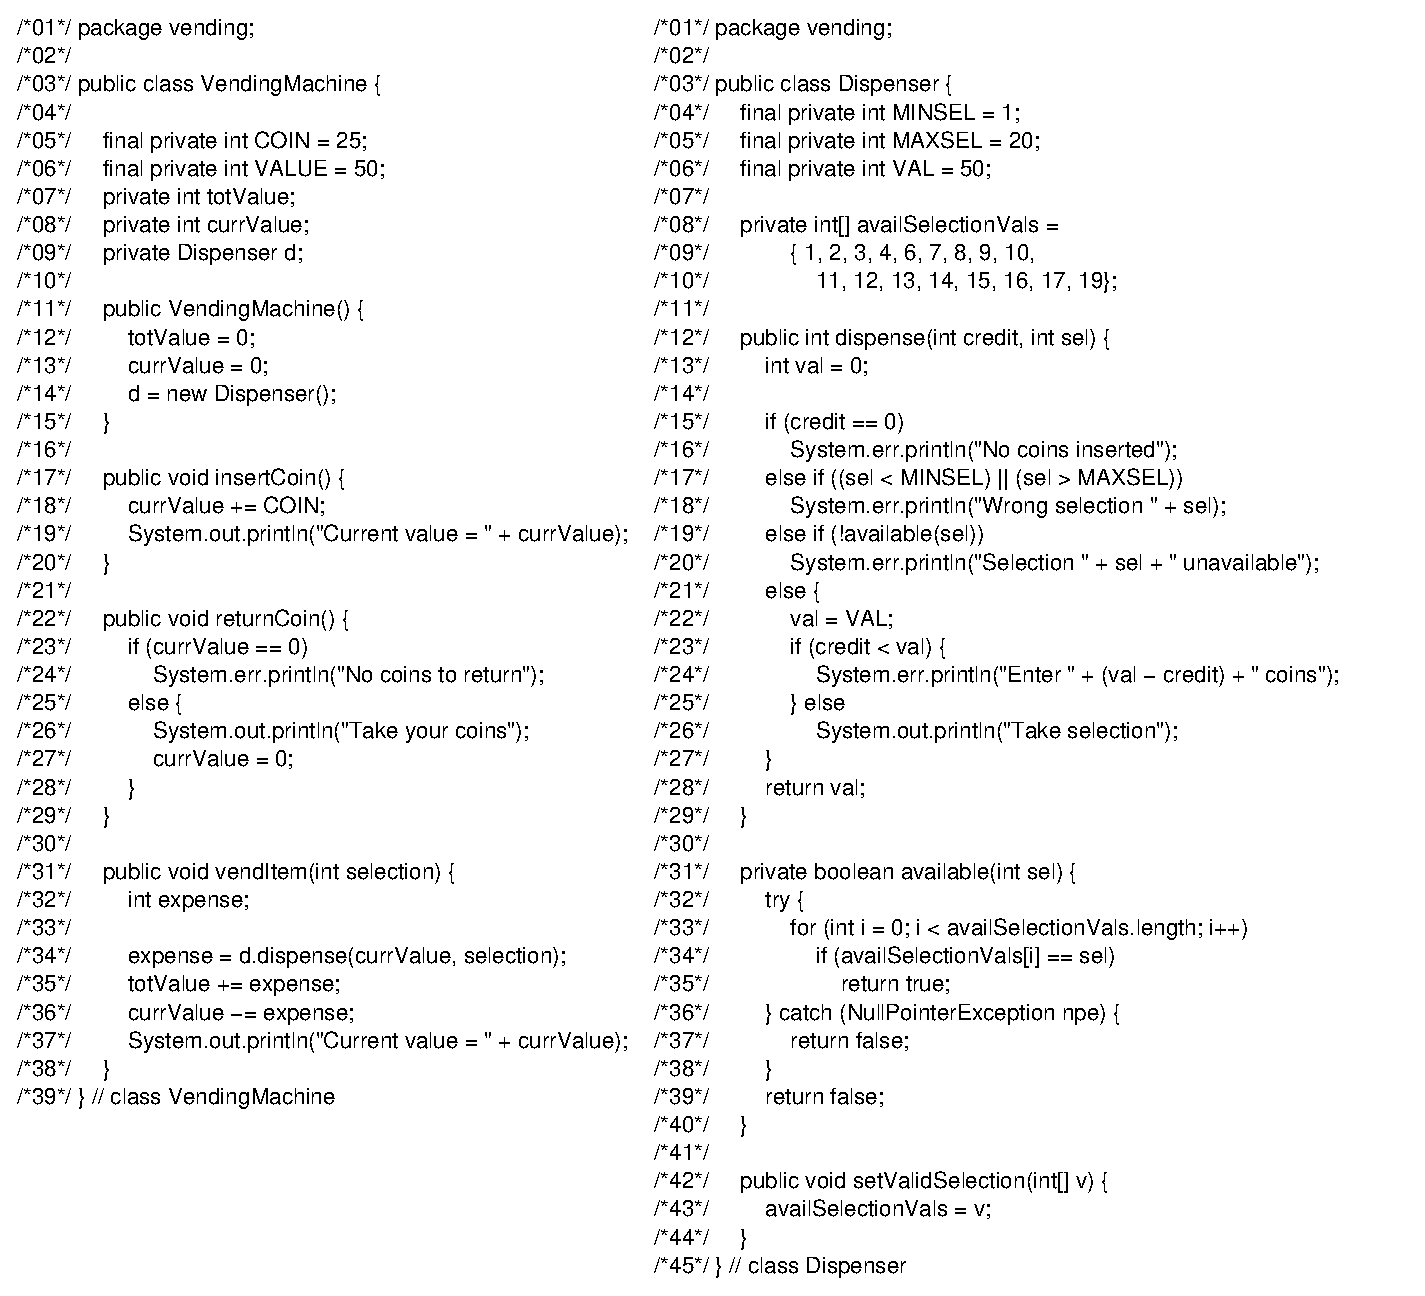
\includegraphics[width=\textwidth]{fig/vending-dispenser.eps}
\caption{\label{fig:vending}Example adapted from~\cite{Orso01UCMS}
of a Java application (\pk{VendingMachine}) and one component
(\pk{Dispenser}).}
\end{center}
\end{figure}


Since neither \pk{VendingMachine} nor \pk{Dispenser} classes have
a \pk{main} method, to allow the invocation of each method of the
\pk{VendingMachine} class, we developed a test driver class
(\pk{TestDriver}) that accepts as input a text file containing a
set of methods' names that have to be executed in the
\pk{VendingMachine} class, creates an instance of
\pk{VendingMachine}, and perform the execution of the required
methods. Figure~\ref{fig:drv} shows the source code of the test
driver.

% This is part of the Jabuti 1.0 Manual.
% Copyright 2003 (c) Auri Marcelo Rizzo Vicenzi, Marcio Eduardo Delamaro,
% Jose Carlos Maldonado.
% See the file FDL.TXT for copying conditions.

\begin{figure}[!ht]
\begin{center}
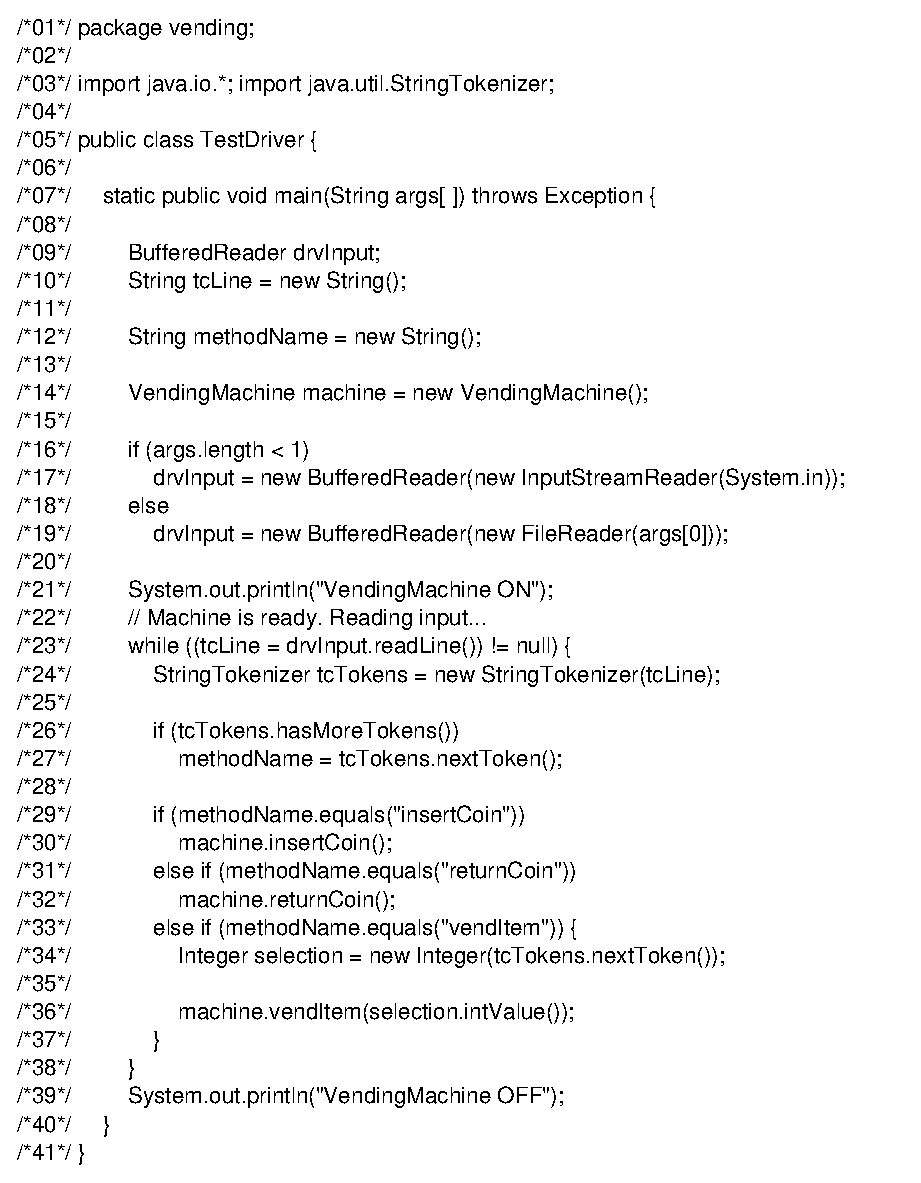
\includegraphics[width=0.6\textwidth]{fig/testdriver.eps}
\caption{\label{fig:drv}Example of a test driver for
\texttt{VendingMachine} and \texttt{Dispenser} classes.}
\end{center}
\end{figure}


For example, considering a typical execution of the vending
machine, a customer insert a certain number of coins, ask to the
vending machine to deliver a given item, and the vending machine
dispenses the required item if it is valid and available. This
steps can be represented by a text file \pk{input1}
(Figure~\ref{fig:input}).

\begin{figure}[!ht]
\begin{cmd}
        insertCoin
        insertCoin
        vendItem 3
\end{cmd}
\vspace{-0.7cm}\caption{A simple test case file:
\pk{input1}.}\label{fig:input}
\end{figure}

By executing the command illustrated in Figure~\ref{fig:driver},
\pk{input1} is read line by line. The first two lines cause the
execution of the method \pk{VendingMachine.insertCoin} twice,
indicating that the customer deposited 50 cents into the vending
machine. The last line corresponds to the choice to buy the item
number three, a valid item that will be delivered to the customer.
Using this approach, valid and invalid test cases can be specified
to check whether the \pk{VendingMachine} application and the
\pk{Dispenser} component behave correctly \wrt their
specifications.

\begin{figure}[!ht]
\begin{cmd}
        java vending.TestDriver input1
\end{cmd}
\vspace{-0.7cm}
\caption{How to execute the implemented test
driver.}\label{fig:driver}
\end{figure}

\rev{Orso \etal~\cite{Orso01UCMS} comment that the source code
presented in Figure~\ref{fig:vending} contains a fault in method
\pk{Dispenser.dispense()}: when a available item is selected and
the credit is insufficient, but greater than zero, the variable
\pk{val} (set to \pk{VAL} at line 22 of \pk{Dispenser} class) is
not set to zero; consequently, when control returns from
\pk{Dispenser.dispense()} to \pk{VendingMachine.vendItem()},
\pk{currValue} is erroneously decremented. To fix this error, the
statement \pk{val = 0} should be included after the statement
located at \pk{Dispenser.dispense()}'s source line 24. Observe
that we will use the faulty version of the \pk{Dispenser}
component to show how the slicing tool (described in
Section~\ref{sec:slice}) can be used to help the localization of
such a fault.}

%------------------------------------------------------------------------------

%----------------------Tool----------------------------------------------------
% This is part of the Jabuti 1.0 Manual.
% Copyright 2003 (c) Auri Marcelo Rizzo Vicenzi, Marcio Eduardo Delamaro,
% Jose Carlos Maldonado.
% See the file FDL.TXT for copying conditions.

\section{\toolname Functionality and Graphical
Interface}\label{sec:tool}

\toolname implements a subset of the functionalities provided by
\xSuds, a complete tool suite for C and C++
programs~\cite{Agrawal98MSTA}. This section describes the
operations that can be performed by \toolname. The graphical
interface allows the beginner to explore and learn the concepts of
control-flow and data-flow testing. Moreover, it provides a better
way to visualize which part of the classes under testing are
already covered and which are not. A general view of the \toolname
graphical interface, including its menus, is presented in
Figure~\ref{fig:tool}. A brief description of each option on each
menu is presented below.

% This is part of the Jabuti 1.0 Manual.
% Copyright 2003 (c) Auri Marcelo Rizzo Vicenzi, Marcio Eduardo Delamaro,
% Jose Carlos Maldonado.
% See the file FDL.TXT for copying conditions.

\begin{figure}[!ht]
\begin{center}
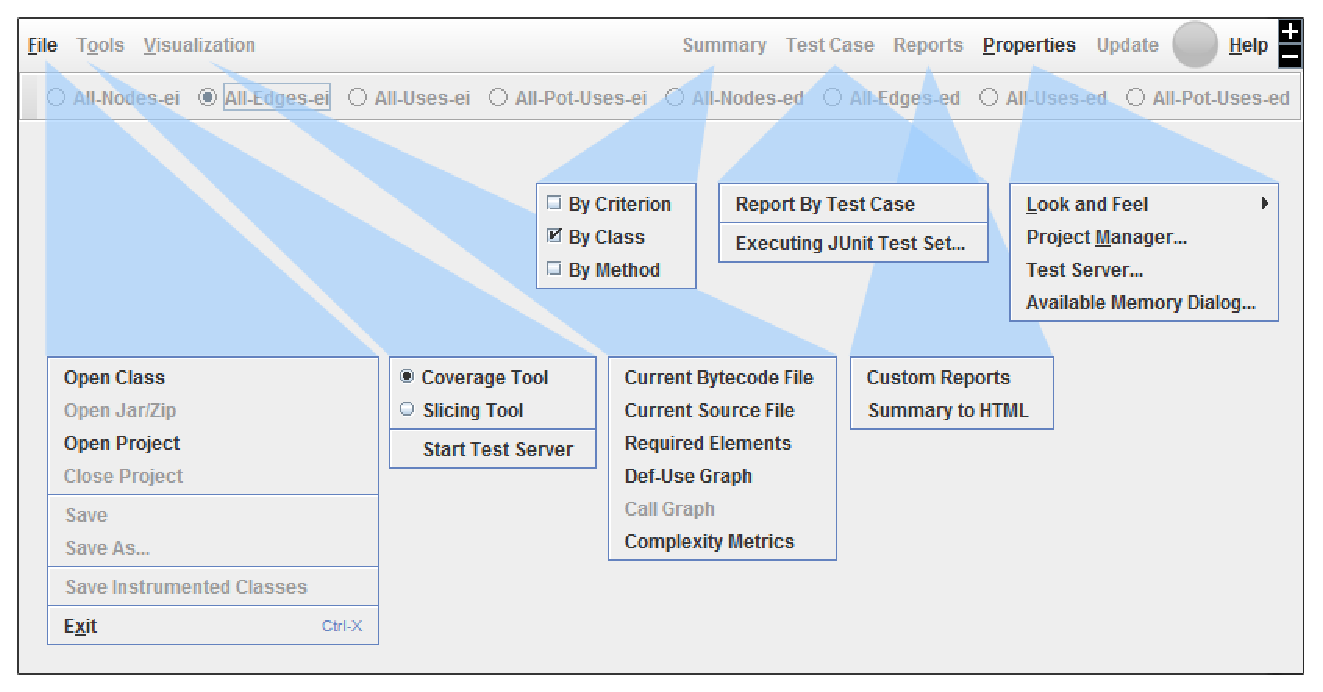
\includegraphics[width=0.7\textwidth]{fig/main-window-editted.eps}
\caption{\label{fig:tool}Operations available in the graphical
interface.}
\end{center}
\end{figure}


\begin{itemize}
    \item \textbf{File Menu} - provides options to create and
    manipulate a \toolname project.
        \begin{itemize}
            \item \textbf{Open Class} - allows to select the base class
            file from where the classes to be tested are
            identified.

            \item \textbf{Open Project} - opens a previously created
            project.

            \item \textbf{Close Project} - closes the current
            project.

            \item \textbf{Save} - saves the current project.

            \item \textbf{Save As} - saves the current project with a different
            name.
            
            \item \textbf{Save Instrumented Classes} - saves the classes from 
            current project, already instrumented for external testing.

            \item \textbf{Exit} - exits of the tool.
        \end{itemize}

    \item \textbf{Tools} - provides the set of tools available in
    \toolname.
        \begin{itemize}
            \item \textbf{Coverage Tool} - enables the \toolname coverage
            tool.

            \item \textbf{Slicing Tool} - enables the \toolname slicing
            tool.
            
            \item \textbf{Start Test Server} - starts the test server for
            mobile devices.

        \end{itemize}

    \item \textbf{Visualization} - provides different forms of
    visualization of the classes and methods under testing.
        \begin{itemize}
            \item \textbf{Current Bytecode File} - shows the highlighted bytecode of the
            current selected class file.

            \item \textbf{Current Source File} - shows the highlighted source code of the
            current selected class file. Observe that this option requires that the source
            code is available to be performed.

            \item \textbf{Required Elements} - shows the set of required elements
            for a given method of a given class, considering the current selected
            criterion (shown below the main menu). The presented
            screen also allows to mark a testing requirement as active/deactive or
            feasible/infeasible.

            \item \textbf{Def-Use Graph} - shows the \DUG
            of a given method of the current class.

            \item \textbf{Complexity Metrics} - shows the resultant value of
            the set of complexity metrics implemented in \toolname for the
            complete set of user classes obtained from the base class.
            This set of classes includes the classes under testing.
        \end{itemize}

    \item \textbf{Summary} - provides personalized coverage information
        in different levels of abstractions.
        \begin{itemize}
            \item \textbf{By Criterion} - shows the cumulative coverage
            information for each testing criterion, considering all classes
            under testing.

            \item \textbf{By Class} - shows the coverage
            information with respect to the current selected criterion,
            for each individual class under testing.

            \item \textbf{By Method} - shows the coverage
            information with respect to the current selected criterion,
            for each individual method of each class under testing.
        \end{itemize}

    \item \textbf{Test Case} - provides options for test set
    manipulation and report generation.
        \begin{itemize}
            \item \textbf{Report By Test Case} - shows the coverage
            information with respect to the current selected criterion,
            for each individual test case, considering all class under
            testing. The presented screen also allows to enable/disable and
            delete/undelete test cases.

%            \item \textbf{Report By Test Case Path} - shows the coverage
%            information with respect to the current selected criterion,
%            for each individual test case path, considering all class under
%            testing.

            \item \textbf{Importing from JUnit} - allows to import a test set
            generated according to the JUnit framework.
        \end{itemize}

    \item \textbf{Reports} - provides options to save \toolname's reports in
    HTML format.
        \begin{itemize}
            \item \textbf{Custom Reports} - allows to generate a custom
            HTML report from the current testing project considering different
            levels of granularity.

            \item \textbf{Summary to HTML} - allows to generate a HTML from
            any tabled style report provided by the \toolname graphical interface.
        \end{itemize}

    \item \textbf{Properties} - provides general configuration options.
        \begin{itemize}
            \item \textbf{Look and Feel} - allows to change the
            look and feel style considering three different options:
            Metal (default), Motif, and Windows.

            \item \textbf{Project Manager...} - allows to verify and change
            the current set of classes under testing in the current project.
            
            \item \textbf{Test Server...} - configuration of the test server.
            
            \item \textbf{Available Memory Dialog...} - shows current available
            memory on system.
        \end{itemize}

    \item \textbf{Update} - provides a visual information every time an
    event that affect the coverage occurs. For example, such a button becomes
    red in case additional test cases are imported or appended in the end of the
    trace file to indicate that a new event that affects the coverage information
    occurs. As soon as it is clicked, its background color changes
    to grey.

    \item \textbf{Help} - provides only one option to show information
    about the authors/developers of \toolname.
\end{itemize}

\toolname requires the creation of a testing project, such that
the tester can specify only once the set of classes to be
instrumented and tested. Section~\ref{sec:project} describes how
to create a \toolname's testing project. After having created the
project, \toolname provides to the tester a coverage analysis
tool, a slicing tool and a static metric measure tool. The
coverage analysis tool is described in Section~\ref{sec:coverage}.
Section~\ref{sec:slice} describes the slicing tool, and
Section~\ref{sec:metrics} describes the measure tool.

%------------------------------------------------------------------------------

%----------------------Session Creation----------------------------------------
% This is part of the Jabuti 1.0 Manual.
% Copyright 2003 (c) Auri Marcelo Rizzo Vicenzi, Marcio Eduardo Delamaro,
% Jose Carlos Maldonado.
% See the file FDL.TXT for copying conditions.

\section{How to Create a Testing Project}\label{sec:project}

In \toolname the testing activity requires the creation of a
testing project. A testing project is characterized by a file
storing the necessary information about (i) the base class file,
(ii) the complete set of classes required by the base class, (iii)
the set of classes to be instrumented (tested), and (iv) the set
of classes that are not under testing. Additional information,
such as the \pk{CLASSPATH} environment variable necessary to run
the base class is also stored in the project file, whose extension
is \prjext. During the execution of any \pk{.class} file that
belongs to the set of classes under testing of a given project,
dynamic control-flow information (execution trace) is collected
and saved in a separate file that has the same name of the project
file but with a different extension (\trcext).

For example, considering the vending machine example, 
%described in Section~\ref{sec:example}, 
the \pk{vending} package is composed by
three \bci{.java} files: \pk{VendingMachine.java},
\pk{Dispenser.java} and \pk{TestDriver.java}. Suppose that these
files are saved in a directory named \verb+~\example+. The
directory structure is like:

\begin{cmd}
auri@AURIMRV ~
$ ls -l example/*
-rw-r--r--    1 auri         1313 Aug  6 09:07 Dispenser.java
-rw-r--r--    1 auri         1340 Aug  6 09:07 TestDriver.java
-rw-r--r--    1 auri          923 Aug  6 09:07 VendingMachine.java
\end{cmd}

To compile such an application one of the following command can be
used:

\begin{cmd}
auri@AURIMRV ~
$ javac -d example example/*.java
\end{cmd}

or

\begin{cmd}
auri@AURIMRV ~
$ javac -g -d example example/*.java
\end{cmd}

Observe that in the later command, the debug option is activated,
thus, the generated \pk{.class} files contains more information,
such as the real variable names. In this report we are using class
files compiled with the debug option.

After the Java source files have been compiled, the
\verb+~\example+ directory contains the following structure:

\begin{cmd}
auri@AURIMRV ~
$ ls -l example/*
-rw-r--r--    1 auri         1313 Aug  6 09:07 Dispenser.java
-rw-r--r--    1 auri         1340 Aug  6 09:07 TestDriver.java
-rw-r--r--    1 auri          923 Aug  6 09:07 VendingMachine.java
example/vending:
vending:
total 6
-rw-r--r--    1 auri         1478 Aug  6 09:49 Dispenser.class
-rw-r--r--    1 auri         1340 Aug  6 09:49 TestDriver.class
-rw-r--r--    1 auri         1253 Aug  6 09:49 VendingMachine.class
\end{cmd}

Now, from the generated \pk{.class} files, the user can create a
project using \toolname. To do this, the first step is to invoke
\toolname's graphical interface. Supposing that \toolname is
installed \rev{on} \verb+~\Tools\jabuti+, the command below causes
the invocation of its graphical interface.

\begin{cmd}
auri@AURIMRV ~/example
$ java -cp ".;..\Tools\jabuti;\
>..\Tools\jabuti\lib\BCEL.jar;\
>..\Tools\jabuti\lib\jviewsall.jar;\
>..\Tools\jabuti\lib\crimson.jar;\
>..\Tools\jabuti\lib\junit.jar" gui.JabutiGUI
\end{cmd}

Observe that the tool requires that some third-party libraries
(BCEL~\cite{Dahm01BCEB} to manipulate the Java bytecode files,
ILOG JViews~\cite{Ilog03JVIE} to visualize the \DUG, Crimson to
manipulate XML files\footnote{Such a package is required when a
java compiler under version 1.4.1 is used (considering the Sun
compiler)).}, and JUnit~\cite{JUnit02UDCA} to import test sets.)
to be included in the \pk{CLASSPATH} to allow its execution. The
current directory, (``.'' in our example), and the base directory
of the tool (\verb+..\Tools\jabuti+) are also included to allow
the correct execution of our example and the tool itself. If
desired, the user can set the \pk{CLASSPATH} environment variable
as a system variable that is initialized during the boot process.
In this case, to call \toolname's GUI, the parameter \pk{-cp} can
be omitted. Figure~\ref{fig:jabuti-initial} illustrates the
\toolname's initial window.

% This is part of the Jabuti 1.0 Manual.
% Copyright 2003 (c) Auri Marcelo Rizzo Vicenzi, Marcio Eduardo Delamaro,
% Jose Carlos Maldonado.
% See the file FDL.TXT for copying conditions.

\begin{figure}[!ht]
\begin{center}
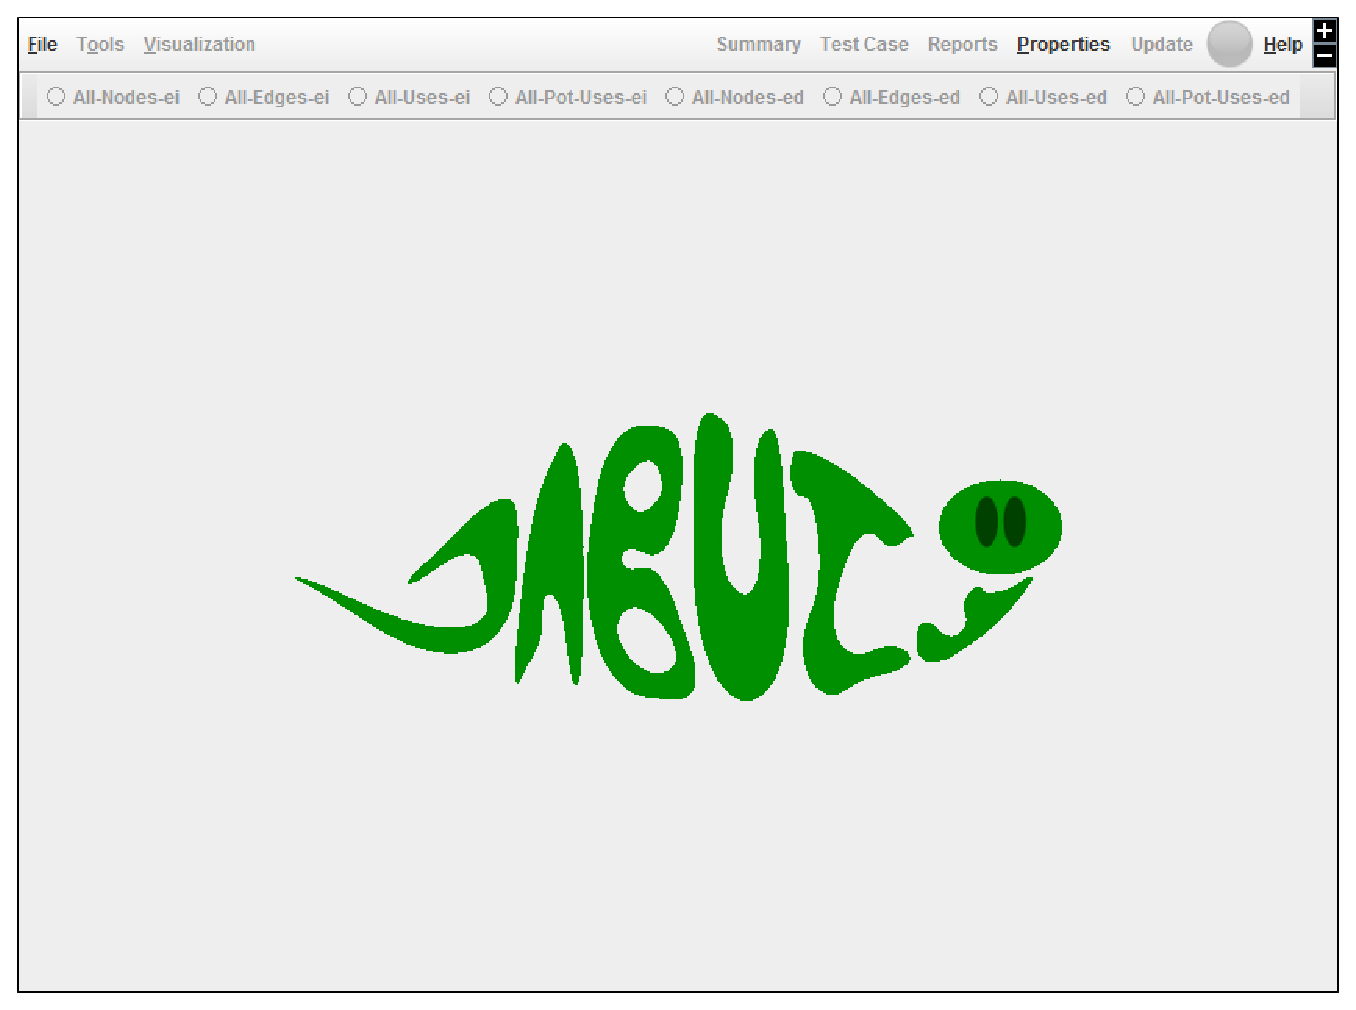
\includegraphics[width=0.70\textwidth]{fig/initial-screen.eps}
\caption{\label{fig:jabuti-initial}\toolname main window.}
\end{center}
\end{figure}


To create a new project, the first step is to select a base
\pk{.class} file from \pk{File $\rightarrow$ Open Class} menu. A
dialog window, as illustrated in
Figure~\ref{fig:project-select-dir} appears. From this dialog
window, the tester selects the directory where the base class file
is located and then select the base class file itself
(Figure~\ref{fig:project-select-class}). Once the base class file
is selected the tool automatically identifies the package that it
belongs (if any) and fills out the \pk{Package} field with the
package's name. The \pk{Classpath} should contains only the path
necessary to run the selected base class. In our example, since
the tool is being called inside the \verb+example+ directory, to
run \pk{vending.TestDriver} it is necessary that the
\pk{Classpath} field contains only the current directory, as shown
in Figure~\ref{fig:project-select-class}.

% This is part of the Jabuti 1.0 Manual.
% Copyright 2003 (c) Auri Marcelo Rizzo Vicenzi, Marcio Eduardo Delamaro,
% Jose Carlos Maldonado.
% See the file FDL.TXT for copying conditions.

\begin{figure}[!ht]
\begin{center}
\subfigure[]{\label{fig:project-select-dir}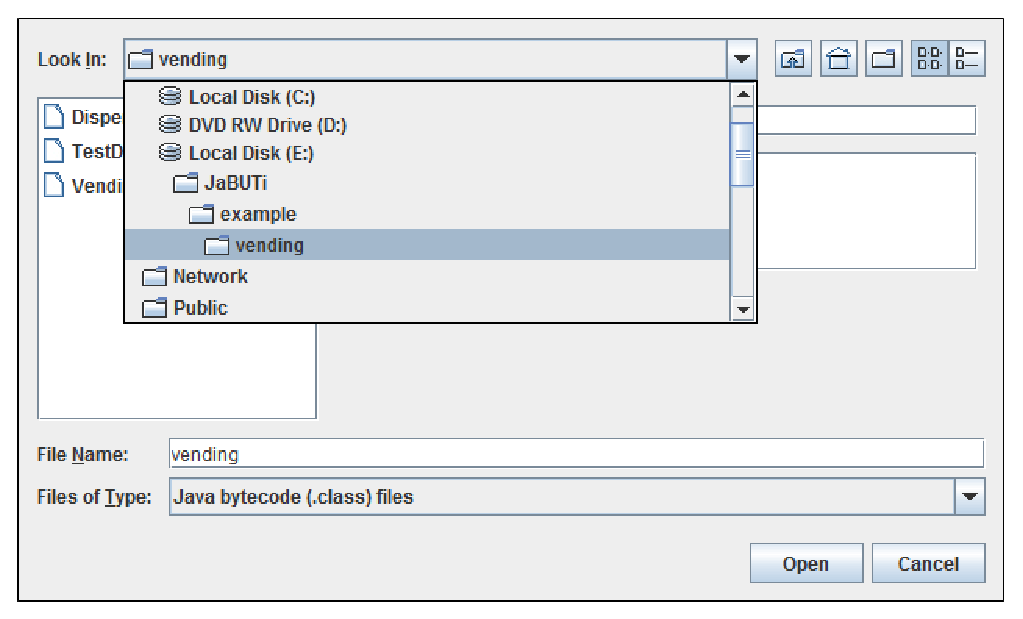
\includegraphics[width=0.45\textwidth]{fig/project-selected-dir.eps}}\qquad
\subfigure[]{\label{fig:project-select-class}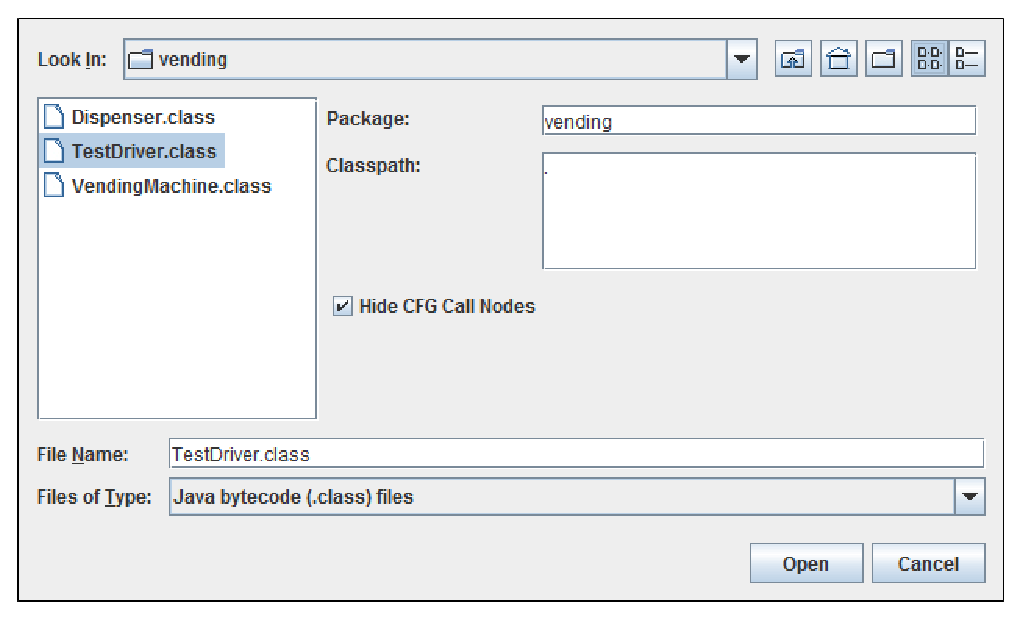
\includegraphics[width=0.45\textwidth]{fig/project-selected-class.eps}}
\caption{Open Class: (a) Selecting the directory and (b) Selecting
the main class file.}\label{fig-jabuti-open-class}
\end{center}
\end{figure}


By clicking the \pk{Open} button
(Figure~\ref{fig:project-select-class}), the \pk{Project Manager}
window, as illustrated in Figure~\ref{fig:project-manager}, will
be displayed. From the selected base class file (\pk{TestDriver}
in our example) the tool identifies the complete set of system and
non-system class files necessary to execute \pk{TestDriver}.
Currently, \toolname does not allows the instrumentation of system
class files. Therefore, the complete set of non-system class files
(user's classes) relate to \pk{TestDriver} can be instrumented.
From the \pk{Project Manager} window (left side) the user can
select the class files that will be tested. At least one class
file must be selected. In our example, we select
\pk{VendingMachine} and \pk{Dispenser} to be instrumented.
\pk{TestDriver} was not selected since it is only the driver that
allows the tester to observe whether the behavior of
\pk{VendingMachine} and \pk{Dispenser} are correct with respect to
their specification.

% This is part of the Jabuti 1.0 Manual.
% Copyright 2003 (c) Auri Marcelo Rizzo Vicenzi, Marcio Eduardo Delamaro,
% Jose Carlos Maldonado.
% See the file FDL.TXT for copying conditions.

\begin{figure}[!ht]
\begin{center}
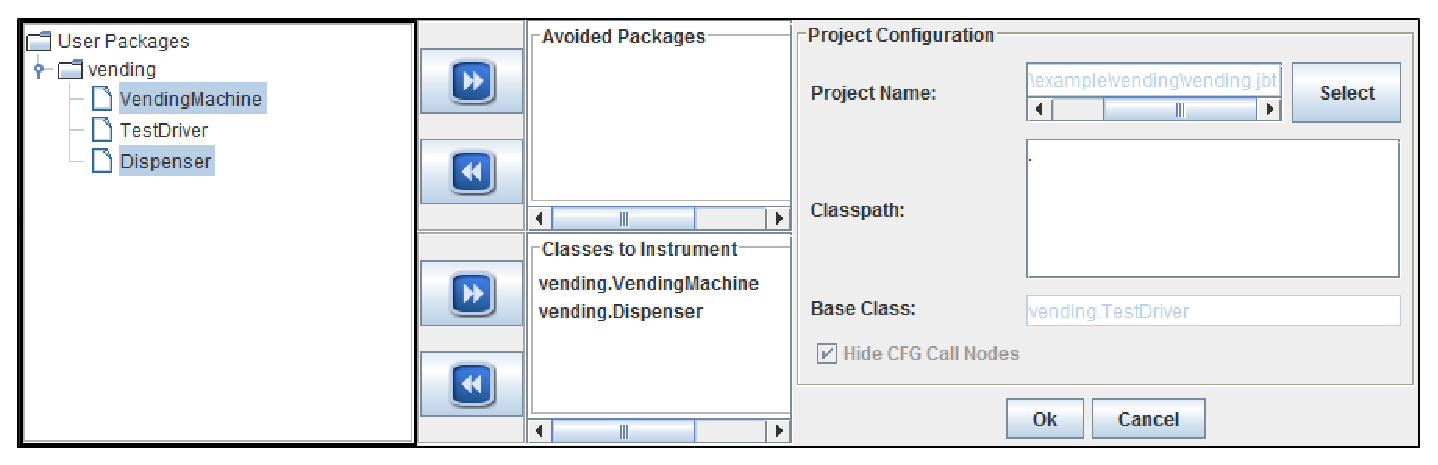
\includegraphics[width=0.90\textwidth]{fig/project-manager.eps}
\caption{\label{fig:project-manager}Selecting the class files to
be tested.}
\end{center}
\end{figure}


Moreover, the tester must give a name to the project being created
(\pk{vending\prjext} in our example) by clicking on the
\pk{Select} button. By clicking on the \pk{Ok} button, \toolname
creates a new project (\pk{vending.jbt} in our example),
constructs the \DUG for each method of each class under testing,
derives the complete set of testing requirements for each
criterion, calculates the weight of each testing requirement, and
presents the bytecode of a given class under testing. By creating
a project, the tester does not need to go through this entire
process again if he/she intends to test the same set of class
files. Next time, he/she can just go to \pk{File $\rightarrow$
Open Project} menu option and reload a previously saved project.

Once the project is created, the tester just need to open it and
the tool automatically detects the classes that compose it.
\toolname can be used for analyzing the coverage of a given class
file, for debugging the class file using the slice tool and for
collecting static metrics information. \toolname also allows the
visualization of the Def-Use Graph (\DUG) of each method in a
given class file as well as the visualization of the source code,
when available. Different kinds of testing reports can also be
generated considering different levels of abstraction. The
following sections describe these features in detail.

%------------------------------------------------------------------------------

%----------------------Coverage Analysis---------------------------------------
% This is part of the Jabuti 1.0 Manual.
% Copyright 2003 (c) Auri Marcelo Rizzo Vicenzi, Marcio Eduardo Delamaro,
% Jose Carlos Maldonado.
% See the file FDL.TXT for copying conditions.

\section{How to use \toolname as a Coverage Analysis
Tool}\label{sec:coverage}

By default, the tool displays the bytecode instead of the Java
source code, since the source code may not be available. The user
can use the \pk{Visualization} menu to change the display to show
the bytecode or source code, as well as the \DUG of each method in
the current class.  As can be observed in
Figure~\ref{fig:dispenser-bytecode}, \toolname uses different
colors to provide hints to the tester to ease the test generation.
The different colors represent requirements with different
weights, and the weights are calculated based on dominator and
super-block analysis~\cite{Agrawal94DSBP}. Informally, the weight
of a testing requirement corresponds to the number of testing
requirements that will be covered if this particular requirement
is covered. Therefore, covering the requirement with the highest
weight will increase the coverage faster\footnote{Observe that the
weight is calculated
        considering only the coverage information
        and should be seen as hints. It does not
        take into account, for instance, the complexity or
        the criticality of a given part of the program. The tester, based on
        his/her experience may desire to cover first a requirement with a
        lower weight but that has a higher complexity or criticality and then,
        after recomputing the weights, uses the hints provided by \toolname to
        increase the coverage faster.}.
The weight schema is used in all views of a given class/method:
bytecode, source code and \DUG.
Figure~\ref{fig:dispenser-bytecode} shows part of the colored
bytecode of the \pk{Dispenser.dispense()} method before the
execution of any test case and Figure~\ref{fig:dispenser-dug} part
of the \DUG of the same method. The different colors correspond to
the weight of each node, considering the \pk{All-Nodes-ei}
criterion. Observe that the color bar (below the main menu) goes
from white (weight 0) to red (weight 7).

In our example, observe that the node 105 in
Figure~\ref{fig:dispenser-dug}, composed by bytecote instructions
from 105 to 112 (Figure~\ref{fig:dispenser-bytecode}), is one of
the highest weight. In this way, a test case that exercises node
105 increases the coverage in at least 7. A requirement with
weight zero is a covered requirement and it is painted in white.

Although the source code is not required by \toolname, when it is
available, the corresponding source code of the current class can
also be displayed in colors, mapped back from the bytecode,
facilitating the identification of which part of the code should
be covered first. For example, Figure~\ref{fig:dispenser-source}
shows that the statements on line 22 and 24 have the highest priority \wrt
the \pk{All-Nodes-ei} criterion. By covering one of these particular
nodes, at least 7 other nodes will be covered.

% This is part of the Jabuti 1.0 Manual.
% Copyright 2003 (c) Auri Marcelo Rizzo Vicenzi, Marcio Eduardo Delamaro,
% Jose Carlos Maldonado.
% See the file FDL.TXT for copying conditions.

\begin{figure}[!ht]
\begin{center}
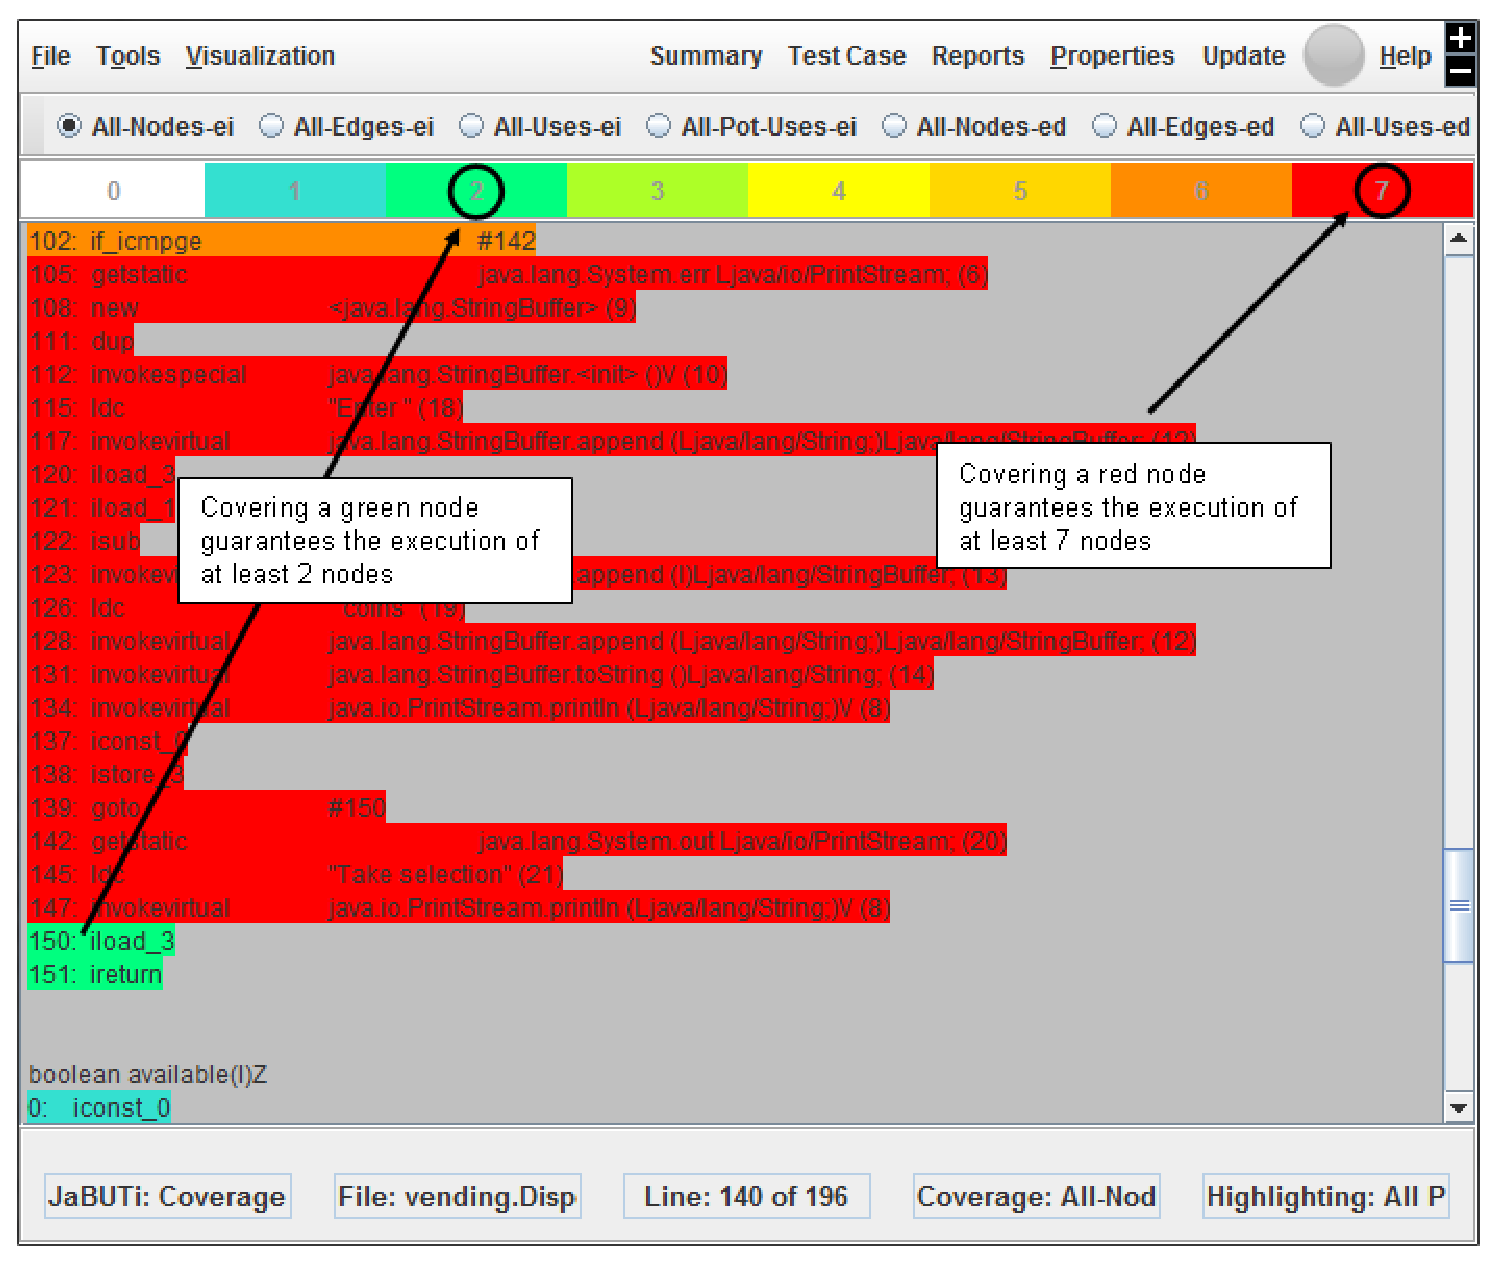
\includegraphics[height=0.40\textheight]{fig/dispenser-bytecode-edited.eps}
\caption{\label{fig:dispenser-bytecode} \pk{Dispenser.dispenser}
method: bytecode prioritized \wrt \pk{All-Pri-Nodes} criterion.}
\end{center}
\end{figure}


% This is part of the Jabuti 1.0 Manual.
% Copyright 2003 (c) Auri Marcelo Rizzo Vicenzi, Marcio Eduardo Delamaro,
% Jose Carlos Maldonado.
% See the file FDL.TXT for copying conditions.

\begin{figure}[!ht]
\begin{center}
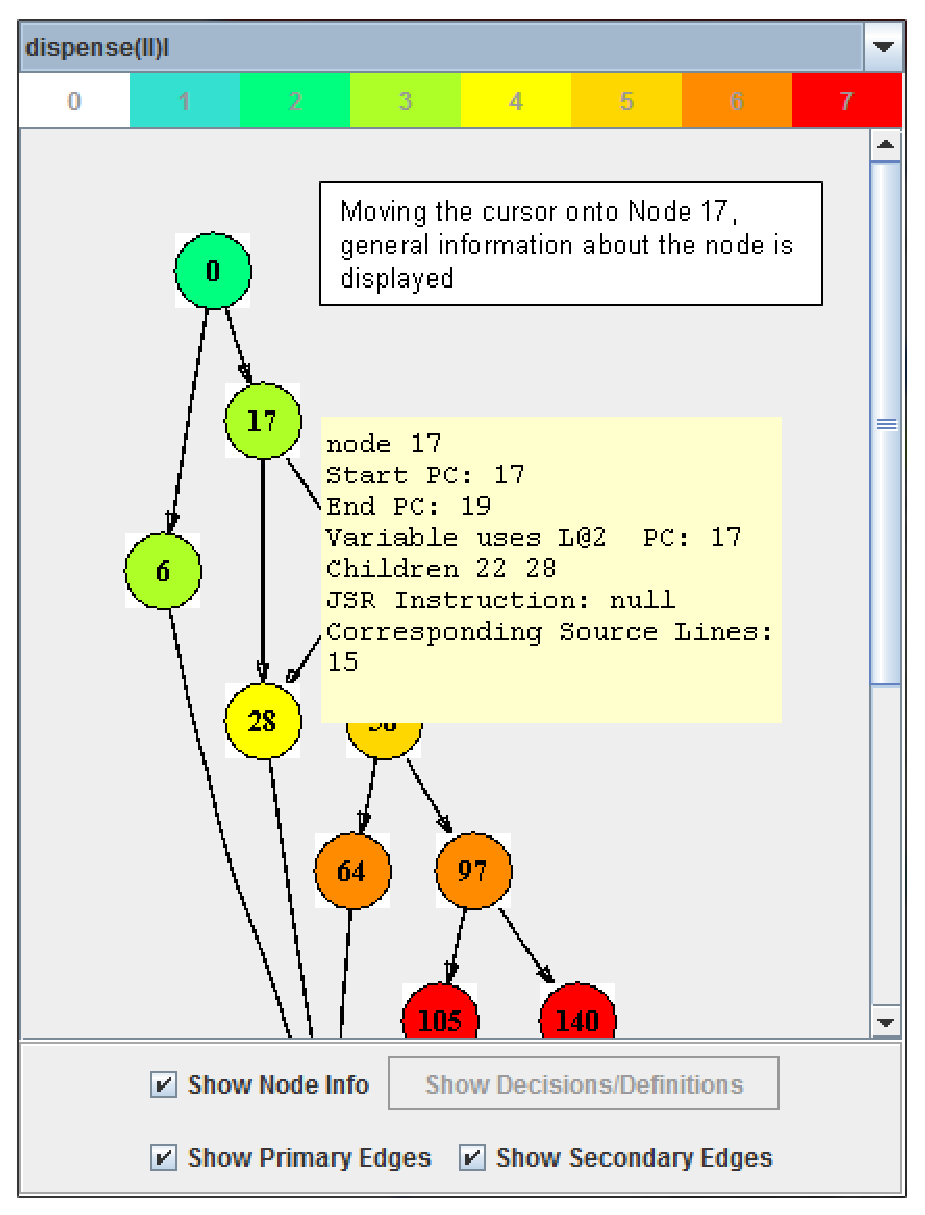
\includegraphics[height=0.35\textheight]{fig/dispenser-dug-edited.eps}
\caption{\label{fig:dispenser-dug} \pk{Dispenser.dispenser}
method: \DUG prioritized \wrt \pk{All-Pri-Nodes} criterion.}
\end{center}
\end{figure}


% This is part of the Jabuti 1.0 Manual.
% Copyright 2003 (c) Auri Marcelo Rizzo Vicenzi, Marcio Eduardo Delamaro,
% Jose Carlos Maldonado.
% See the file FDL.TXT for copying conditions.

\begin{figure}[!ht]
\begin{center}
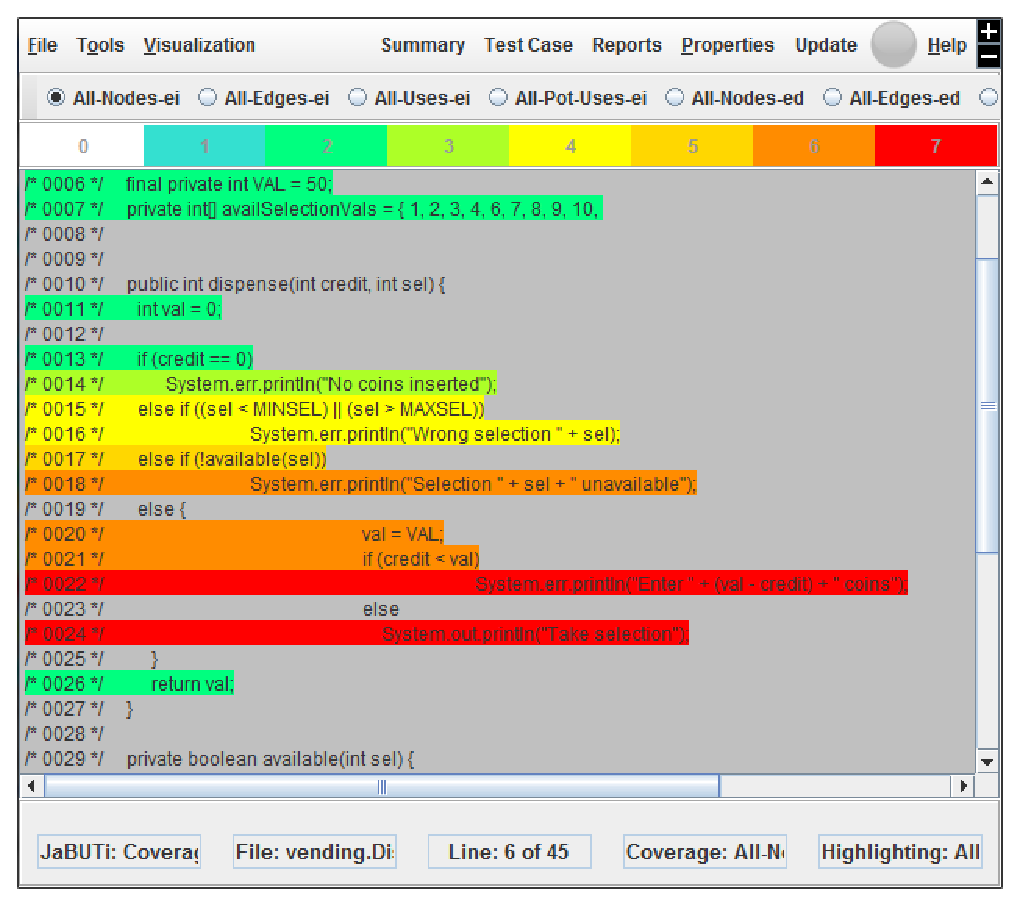
\includegraphics[height=0.40\textheight]{fig/dispenser-source.eps}
\caption{\label{fig:dispenser-source} \pk{Dispenser.dispenser}
method: source code prioritized \wrt \pk{All-Pri-Nodes}
criterion.}
\end{center}
\end{figure}


%Considering the \DUG presented in Figure~\ref{fig:dispenser-dug},
%it can be observed that 
There are two different types of nodes,
represented by single and double line circles. 
%As described in Section~\ref{sec:dependence}, 
Double circles represent call nodes,
\ie, nodes where exists a method call to another method. This
nodes are identified since we intend to extend our tool to deal,
not only with intra-method testing criteria, but also with
inter-method testing criteria that requires the identification of
the relationship among methods. Bold circles, not visible in
Figure~\ref{fig:dispenser-dug}, represent exit nodes. Observe that
methods in Java can have more that one exit node due to the
exception-handling mechanism. All the other nodes are represented
as single line circles. We also have two different types of edges
to represent the ``normal'' control-flow (continuous line --
Primary Edges) and exception control-flow (dashed lines --
Secondary Edges). Figure~\ref{fig:dispenser-dug} does not contain
exception edges. Primary and secondary edges can be hidden by
deselecting the \pk{Show Primary} and \pk{Show Secondary Edges}
check box, respectively. The node information shown when the
cursor is moved onto the node, as illustrated in
Figure~\ref{fig:dispenser-dug}, can also be disabled by
deselecting the \pk{Show Node Info} check box.

\subsection{How the testing requirements are highlighted}

As can be observed above the main menu in
Figure~\ref{fig:dispenser-bytecode}, \toolname supports the
application of six structural testing criteria:
%, as described in Section~\ref{sec:criteria}
All-Nodes-ei, All-Nodes-ed,
All-Edges-ei, All-Edges-ed, All-Uses-ei, and All-Uses-ed.
Depending on which criterion is active, the bytecode, source code
or \DUG is colored in a different way.
Figures~\ref{fig:dispenser-bytecode}, \ref{fig:dispenser-dug},
and~\ref{fig:dispenser-source} show the color schema considering
the \pk{All-Nodes-ei} criterion, which is the same as the
\pk{All-Nodes-ed}, i.e., for these criteria, each requirement is
a node, therefore, since each node has its own weight, the
complete bytecode, source code or \DUG appears highlighted
according to the weight of each node.

Considering the \pk{All-Edges-ei} and \pk{All-Edges-ed}
criteria, their requirements (\DUG edges) are colored using a
2-layer approach. For \pk{All-Edges-ei} criterion, only the nodes
with more than one out-going edge (decision nodes) are painted in
the first layer. For example, Figure~\ref{fig:decision-color}
shows part of the decision nodes of method
\pk{Dispenser.dispense()} and how they are painted in the first
layer. For each decision node, its weight is the maximum weight of
its branches. Suppose a decision node has two branches: one has a
weight of 2 and the other has a weight of 7. The weight of this
decision node is 7. 
%This is the case of \DUG node 61, in our example. 
A decision node has a zero weight if and only if all its
branches are covered. Such decisions are highlighted in white.
Observe that, in the bytecode view, only the last bytecode
instruction of a decision node is highlighted, not the entire node
as the \pk{All-Nodes-ei} and the \pk{All-Nodes-ed} criteria. For
example, \DUG decision node 22 goes from offset 22 to 25,
although, in the bytecode view, only bytecode instruction at
offset 25 is highlighted.

% This is part of the Jabuti 1.0 Manual.
% Copyright 2003 (c) Auri Marcelo Rizzo Vicenzi, Marcio Eduardo Delamaro,
% Jose Carlos Maldonado.
% See the file FDL.TXT for copying conditions.

\begin{figure}[!ht]
\begin{center}
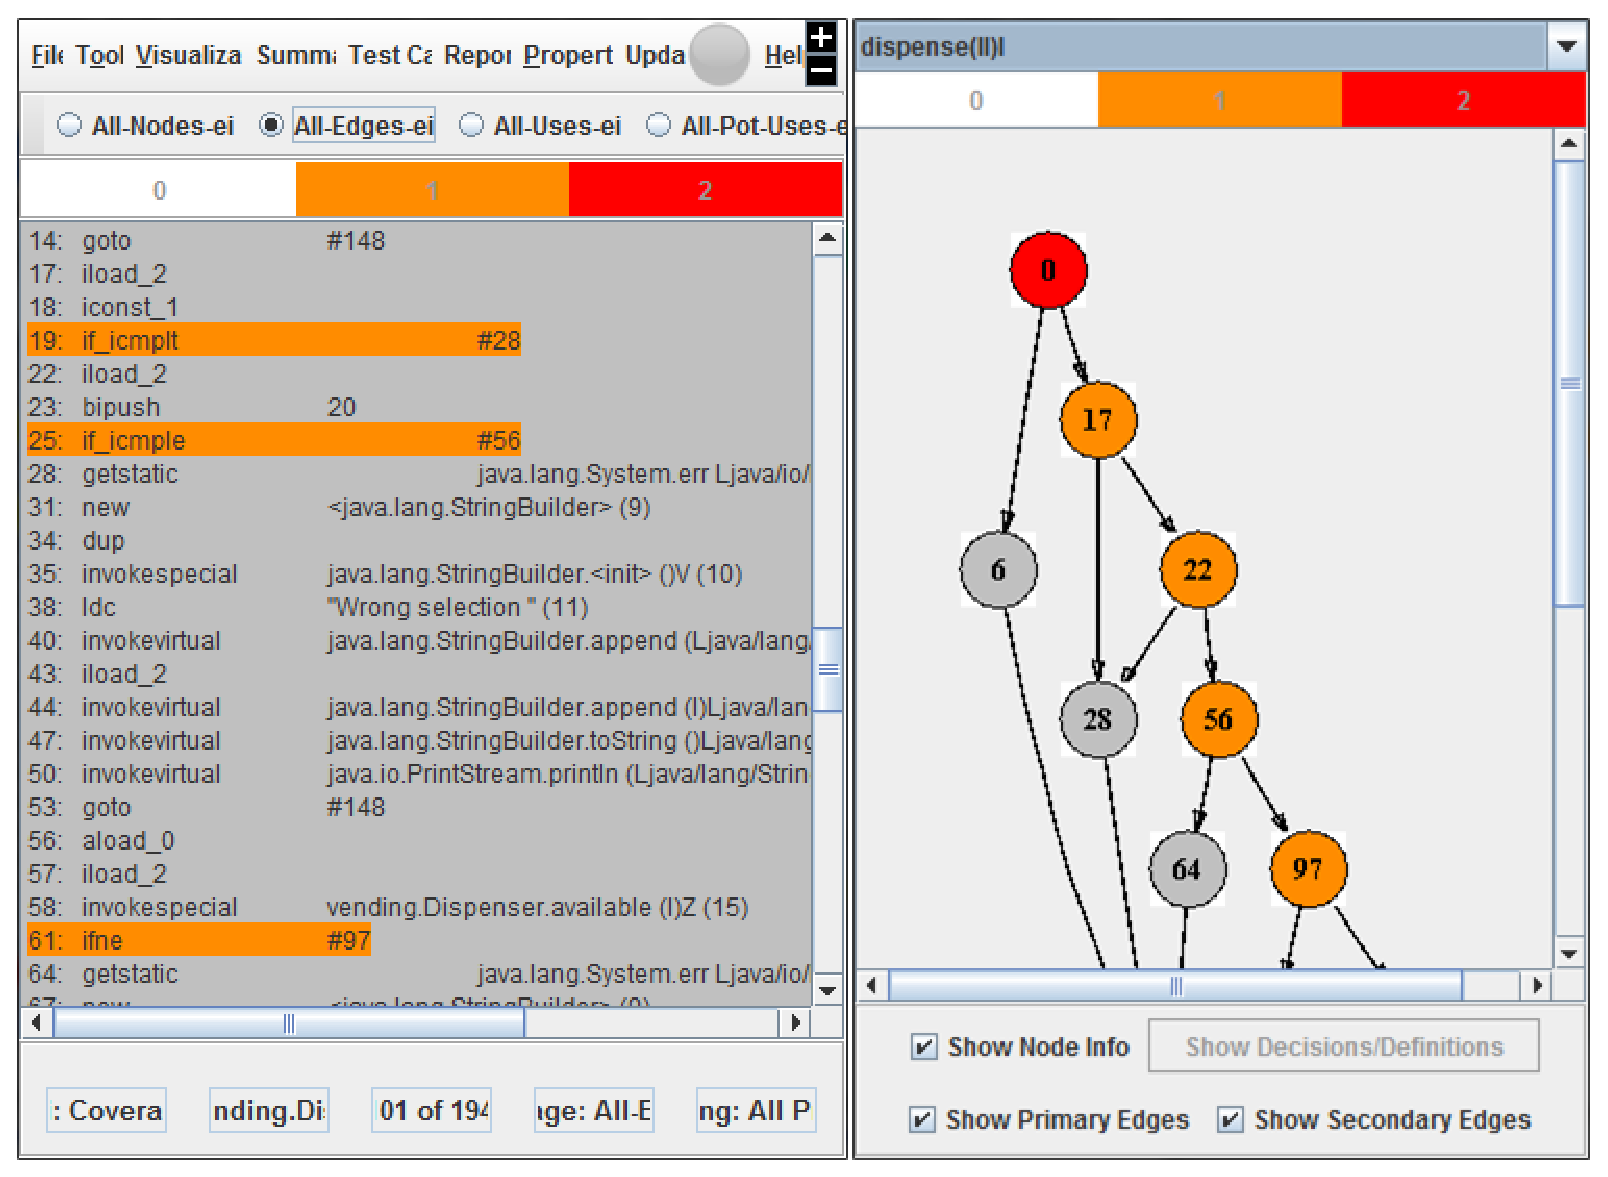
\includegraphics[height=0.40\textheight]{fig/decision-layer1.eps}
\caption{\label{fig:decision-color} Color schema for
\pk{All-Pri-Edges} criterion: first layer.}
\end{center}
\end{figure}


By clicking either in a colored bytecode instruction or in a \DUG
node, all destination nodes of the branches associated with the
selected decision node are highlighted and the decision node
itself changes to a different color. For example, by clicking on
the decision node with the highest weight (node 0 in the
example), its children (nodes 6 and 17) are highlighted in
different colors, considering their individual weights: node 6
has a weight of 2 (red) and node 17 has a weight of 1 (orange),
as illustrated in Figure~\ref{fig:decision-color2}. Therefore, to
improve the coverage with respect to the \pk{All-Edges-ei}
criterion, the tester should exercises first the edge
\edg{0}{6}, since it has the highest weight.

% This is part of the Jabuti 1.0 Manual.
% Copyright 2003 (c) Auri Marcelo Rizzo Vicenzi, Marcio Eduardo Delamaro,
% Jose Carlos Maldonado.
% See the file FDL.TXT for copying conditions.

\begin{figure}[!ht]
\begin{center}
\includegraphics[height=0.40\textheight]{fig/decision-layer2.eps}
\caption{\label{fig:decision-color2} Color schema for
\pk{All-Pri-Edges} criterion: second layer.}
\end{center}
\end{figure}


\rev{Observe that, in case a given method has no decision node,
only the entry node is painted in the first layer and its child in
the second layer. In this case, edges criterion is equivalent to
nodes criterion, since, in a normal execution, once the entry node
is exercised, all the other nodes and edges are.}
Figure~\ref{fig:no-decision} illustrates how the \DUG of the
default constructor of the class \pk{VendingMachine}
(\pk{VendingMachine.init()}) is highlighted before
(Figure~\ref{fig:no-decision-1}) and after
(Figure~\ref{fig:no-decision-2}) the node selection.

% This is part of the Jabuti 1.0 Manual.
% Copyright 2003 (c) Auri Marcelo Rizzo Vicenzi, Marcio Eduardo Delamaro,
% Jose Carlos Maldonado.
% See the file FDL.TXT for copying conditions.

\begin{figure}[!ht]
\begin{center}
\subfigure[]{\label{fig:no-decision-1}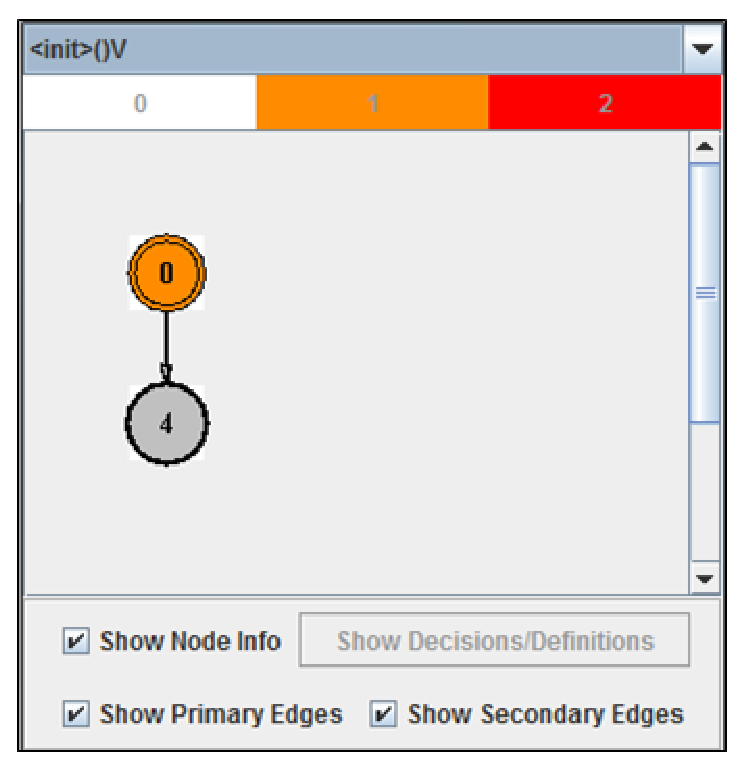
\includegraphics[width=0.45\textwidth]{fig/special-pri-edges-layer1.eps}}\qquad
\subfigure[]{\label{fig:no-decision-2}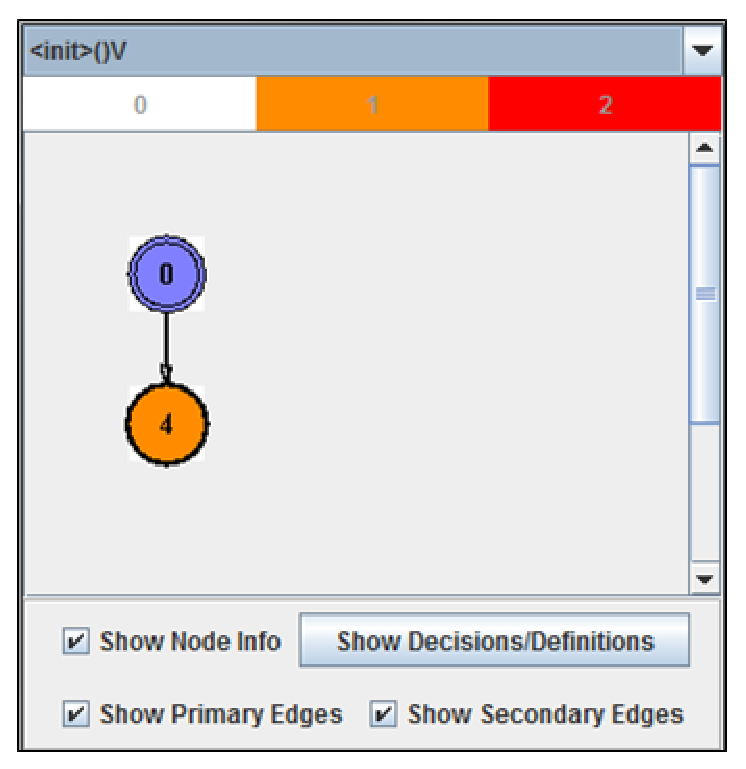
\includegraphics[width=0.45\textwidth]{fig/special-pri-edges-layer2.eps}}
\caption{Special case when no decision node is
found.}\label{fig:no-decision}
\end{center}
\end{figure}


For the \pk{All-Edges-ed} criterion, the same approach is used.
In the first layer, all nodes with at least one secondary
out-going edge, instead of decision nodes, are highlighted. For
each such a node, its weight is the maximum weight of its branches
and a node with more that one secondary out-going edge is
considered covered (zero weight) if and only if all
exception-handler associated with such a node is covered.

Figure~\ref{fig:sec-edges-1} and~\ref{fig:sec-edges-2} shows the
first and the second layer of \pk{Dispenser.available()} method,
considering the \pk{All-Edges-ed} criterion, respectively. In
this example, in the first layer, all highlighted nodes has the
same weigh (one) since it has only one valid exception-handler for
the entire method. In the bytecode view, only the last bytecode
instruction of each node is highlighted. For example, node 2 goes
from offset 2 to 8, therefore, bytecode instruction at offset 8
is highlighted. By clicking on such an instruction or on the \DUG
node 2, Figure~\ref{fig:sec-edges-2} shows the resultant color
schema of the second layer.

% This is part of the Jabuti 1.0 Manual.
% Copyright 2003 (c) Auri Marcelo Rizzo Vicenzi, Marcio Eduardo Delamaro,
% Jose Carlos Maldonado.
% See the file FDL.TXT for copying conditions.

\begin{figure}[!ht]
\begin{center}
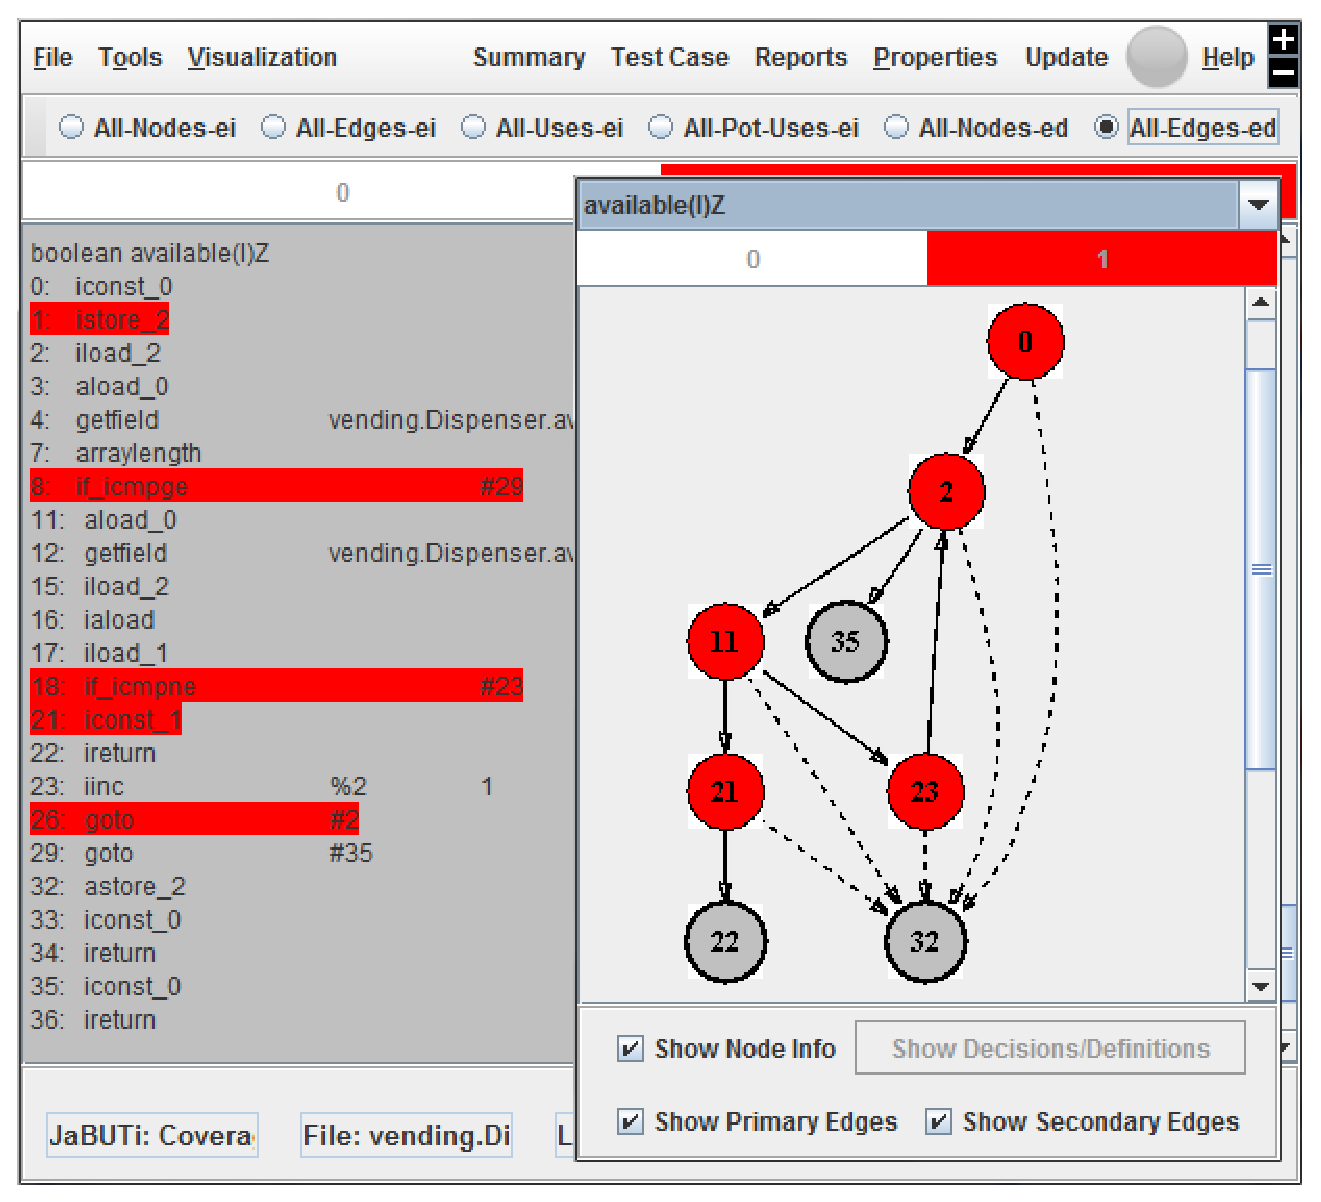
\includegraphics[height=0.40\textheight]{fig/sec-edges-layer1.eps}
\caption{\label{fig:sec-edges-1} Color schema for
\pk{All-Sec-Edges} criterion: first layer.}
\end{center}
\end{figure}


% This is part of the Jabuti 1.0 Manual.
% Copyright 2003 (c) Auri Marcelo Rizzo Vicenzi, Marcio Eduardo Delamaro,
% Jose Carlos Maldonado.
% See the file FDL.TXT for copying conditions.

\begin{figure}[!ht]
\begin{center}
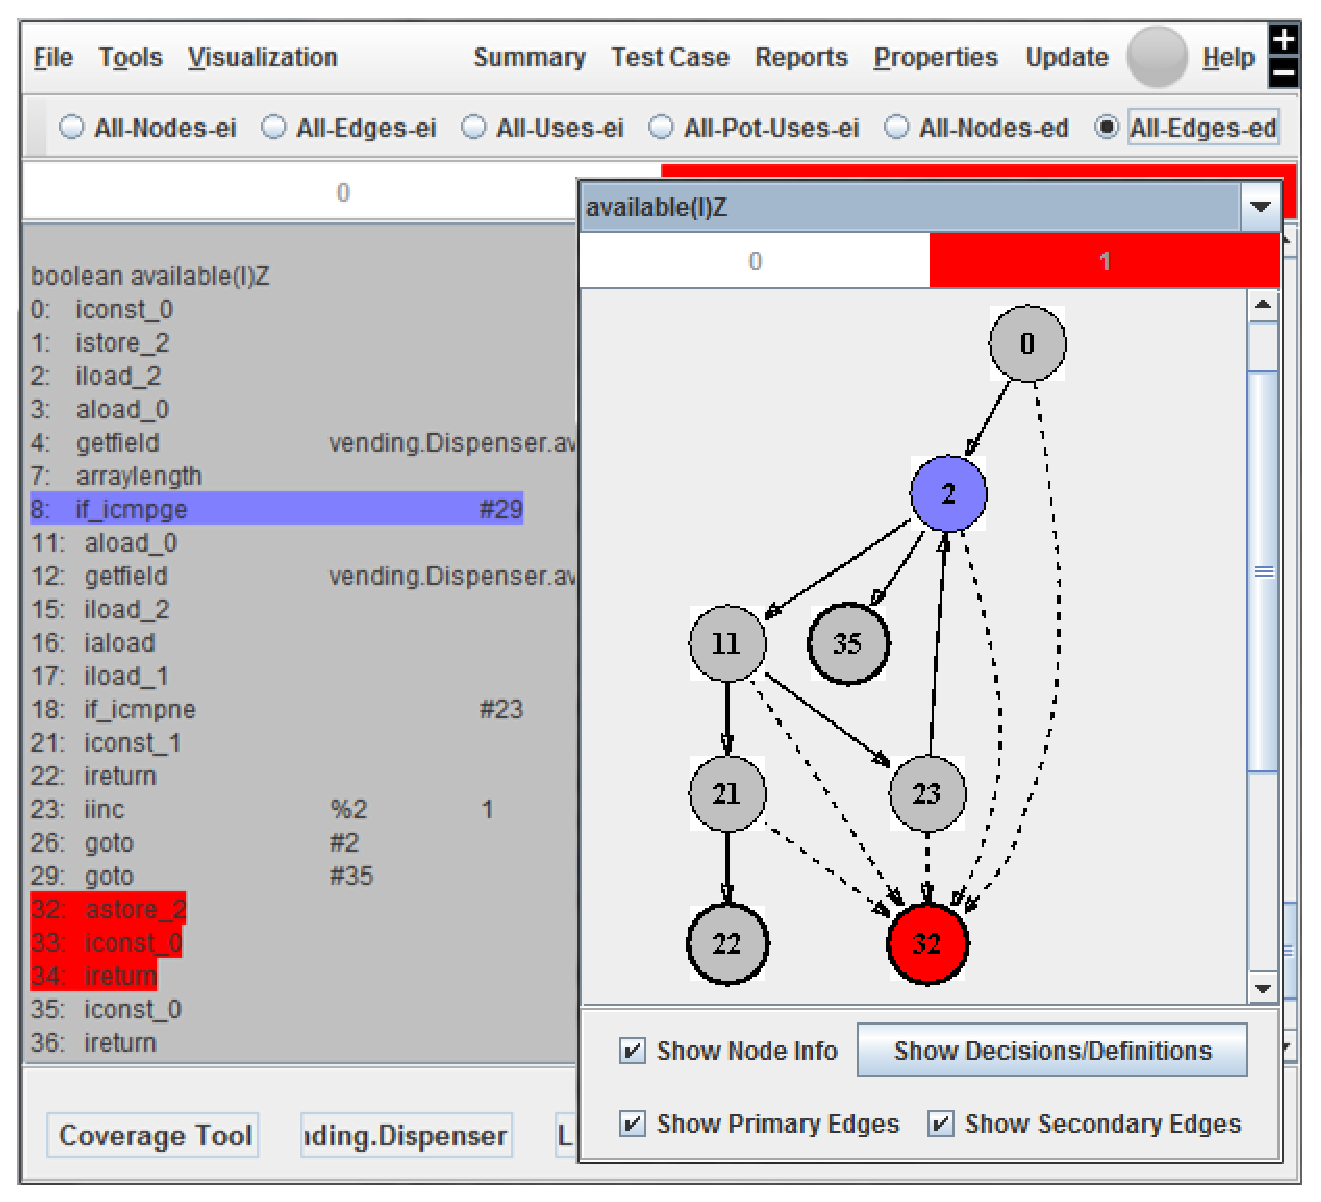
\includegraphics[height=0.40\textheight]{fig/sec-edges-layer2.eps}
\caption{\label{fig:sec-edges-2} Color schema for
\pk{All-Sec-Edges} criterion: second layer.}
\end{center}
\end{figure}


Similar to a decision and its branches are displayed, a 2-layer
representation is also used to display def-use associations for
the \pk{All-Uses-ei} and \pk{All-Uses-ed} criteria. The first
layer shows all the definitions which have at least one c-use or
p-use association. Clicking on a definition goes to the second
layer displaying all c-use and p-use associated with the selected
definition. For each definition, its weight is the maximum weight
of its c-uses or p-uses. For example, suppose a definition has
three def-use associations, one c-use and two p-uses, and the
weights of these associations are 5, 3 and 7, respectively. The
weight of this definition is 7. A definition has a zero weight if
and only if all its c-uses and p-uses are covered. Such
definitions are displayed with a white background.

Since even in the bytecode, more than one variable may be defined
in the same offset, if desired, by clicking with the right mouse
button over a definition point (bytecode offset, source code line
or \DUG node), a pop-up menu is opened showing all the variables
defined in that point such that it is possible to choose which
variable definition to select. For example,
Figure~\ref{fig:uses-color} shows the set of defined variables at
bytecode offset 0 that is part of the \DUG node 0. Observe that in
the \DUG node 0 there is one additional variable definition
because \pk{L@3 (val)} is defined at bytecode offset 1 that also
belongs to \DUG node 0. When a definition point is clicked with
the left mouse button the definition with the highest weight is
considered selected. If all of then have the same weight, the
first is selected. In our example, supposing that \pk{L@1
(credit)} is selected (the definition with the highest weight),
Figure~\ref{fig:uses-color2} shows some of its uses (p-uses in
this case) with the corresponding weight.

% This is part of the Jabuti 1.0 Manual.
% Copyright 2003 (c) Auri Marcelo Rizzo Vicenzi, Marcio Eduardo Delamaro,
% Jose Carlos Maldonado.
% See the file FDL.TXT for copying conditions.

\begin{figure}[!ht]
\begin{center}
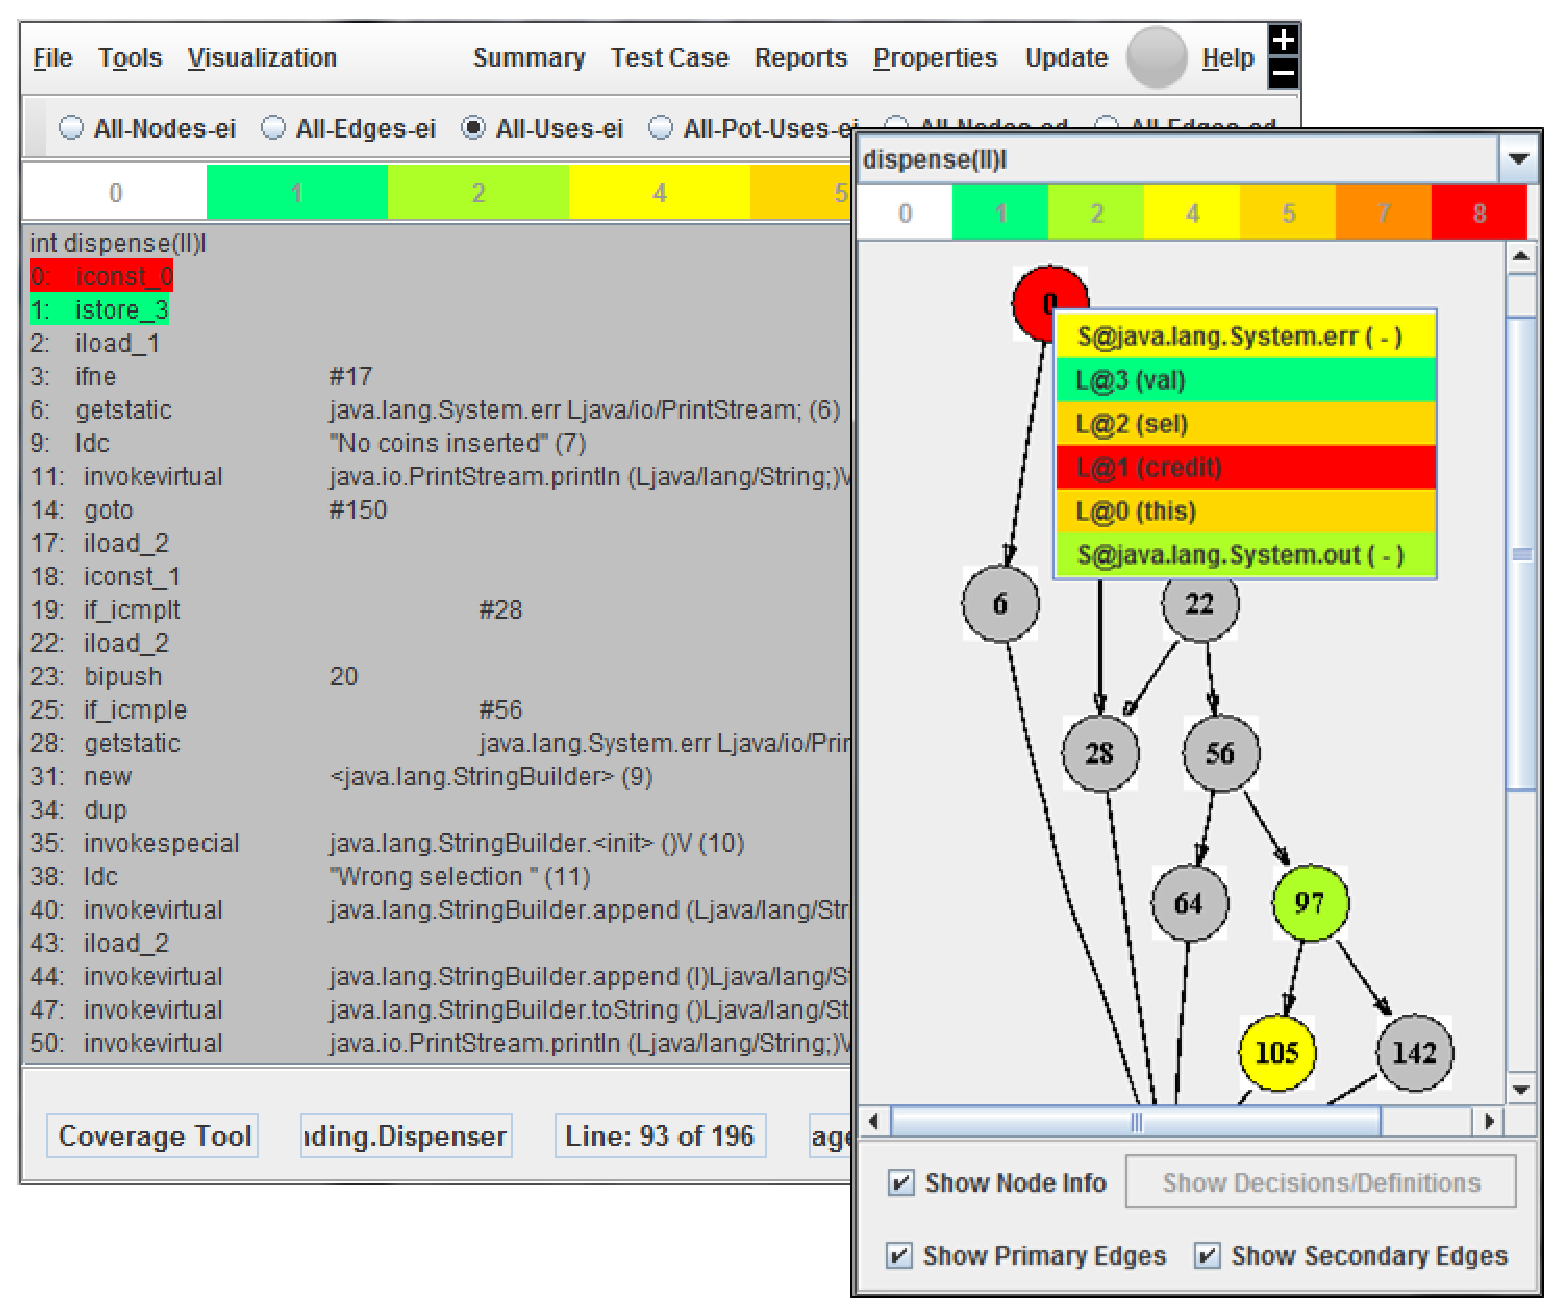
\includegraphics[height=0.40\textheight]{fig/pri-uses-layer1.eps}
\caption{\label{fig:uses-color} Color schema for \pk{All-Pri-Uses}
criterion: first layer.}
\end{center}
\end{figure}


% This is part of the Jabuti 1.0 Manual.
% Copyright 2003 (c) Auri Marcelo Rizzo Vicenzi, Marcio Eduardo Delamaro,
% Jose Carlos Maldonado.
% See the file FDL.TXT for copying conditions.

\begin{figure}[!ht]
\begin{center}
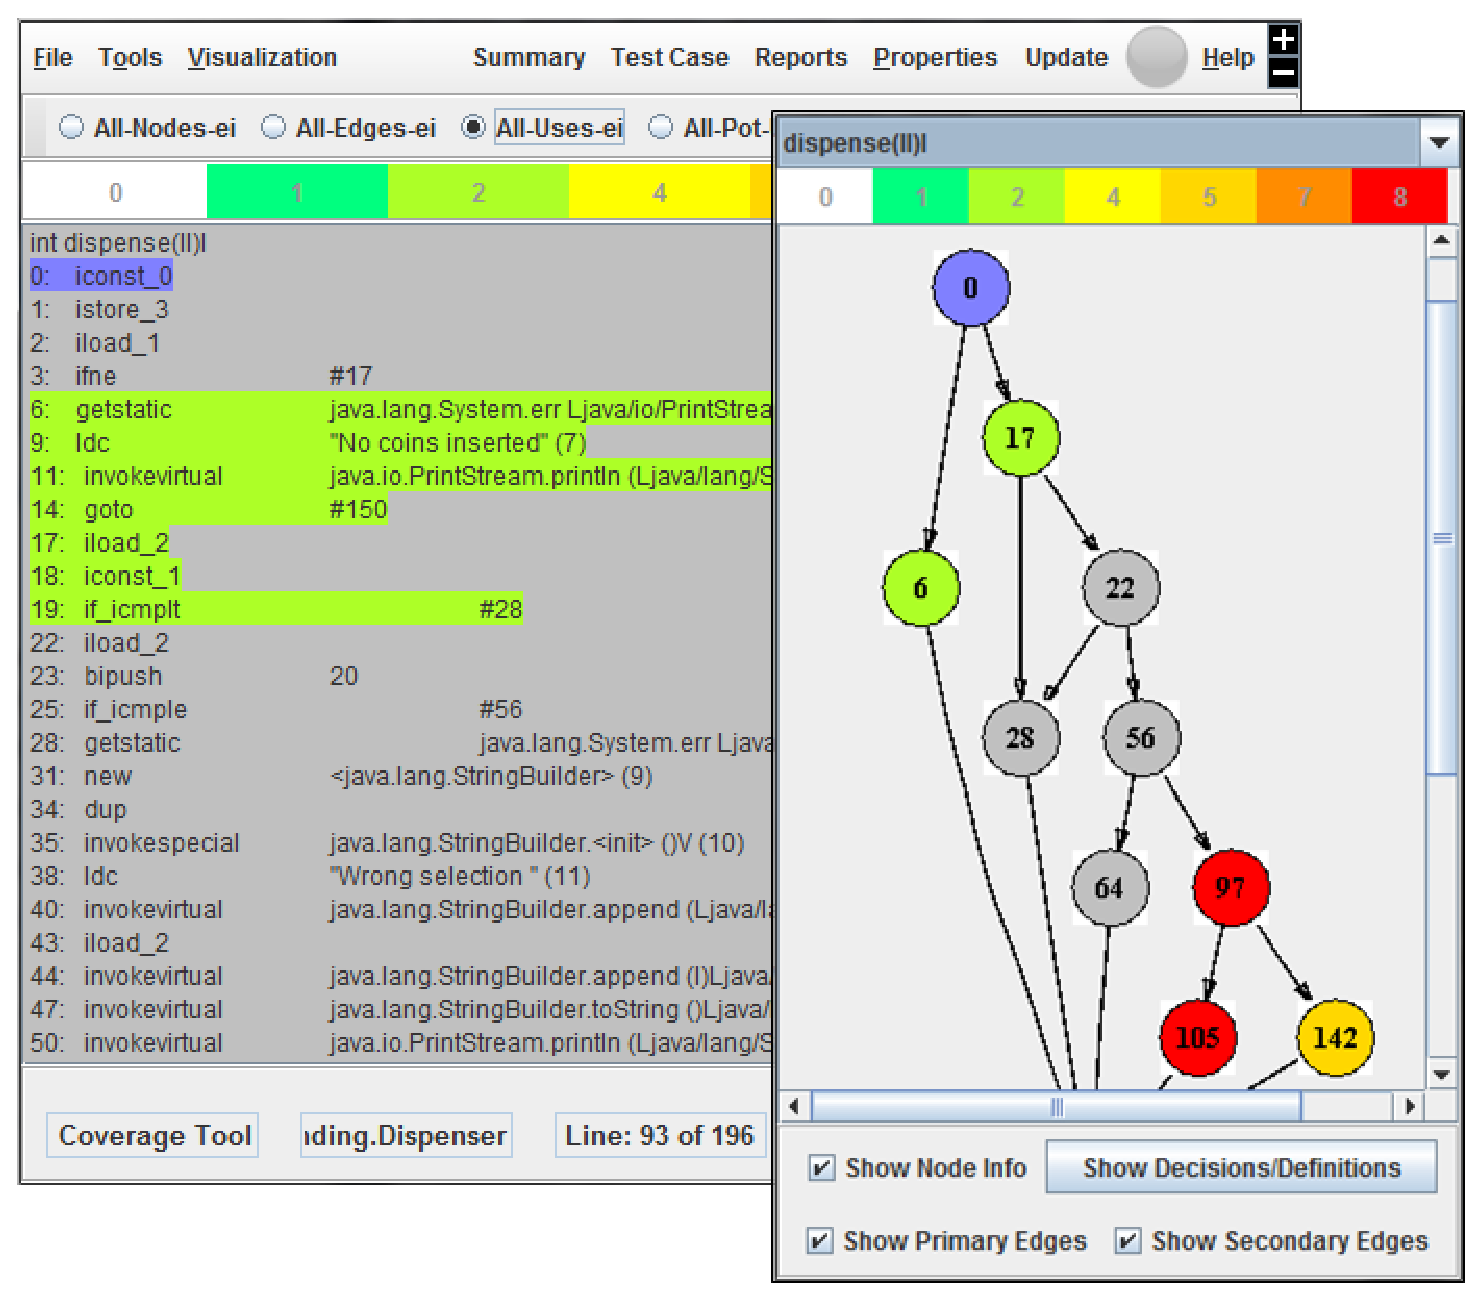
\includegraphics[height=0.40\textheight]{fig/pri-uses-layer2.eps}
\caption{\label{fig:uses-color2} Color schema for
\pk{All-Pri-Uses} criterion: second layer.}
\end{center}
\end{figure}


It is important to observe that the weights provided by the tool
may be seen as hints for the tester to facilitate the generation
of test cases, such that a higher coverage can be obtained with
fewer test cases. Since the prioritization does not consider the
criticality of a given part of the code, if desired, the tester
may choose a different part of the code to be tested first based
on his/her knowledge about the application, even if such a part
has a lower weight than other parts of the code. After the
critical parts have to be tested, additional test cases can be
developed considering the hints.

\subsection{How to generate testing reports}

To evaluate the coverage obtained, the tool provides personalized
tabled style testing reports that can be accessed from the
\pk{Summary} and \pk{Test Case} menus. Any tabled style report can
be saved as a HTML file by accessing \pk{Reports $\rightarrow$
Summary to HTML} menu option. The tool provides reports \wrt each
testing criterion (\pk{Summary $\rightarrow$ By Criterion}), \wrt
each class file (\pk{Summary $\rightarrow$ By Class}) and \wrt
each method (\pk{Summary $\rightarrow$ By Method}).
Figures~\ref{fig:initial-summary-criterion},
\ref{fig:initial-summary-class},
and~\ref{fig:initial-summary-method} show each one of these
reports, respectively, considering that no test case have been
executed.

% This is part of the Jabuti 1.0 Manual.
% Copyright 2003 (c) Auri Marcelo Rizzo Vicenzi, Marcio Eduardo Delamaro,
% Jose Carlos Maldonado.
% See the file FDL.TXT for copying conditions.

\begin{figure}[!ht]
\begin{center}
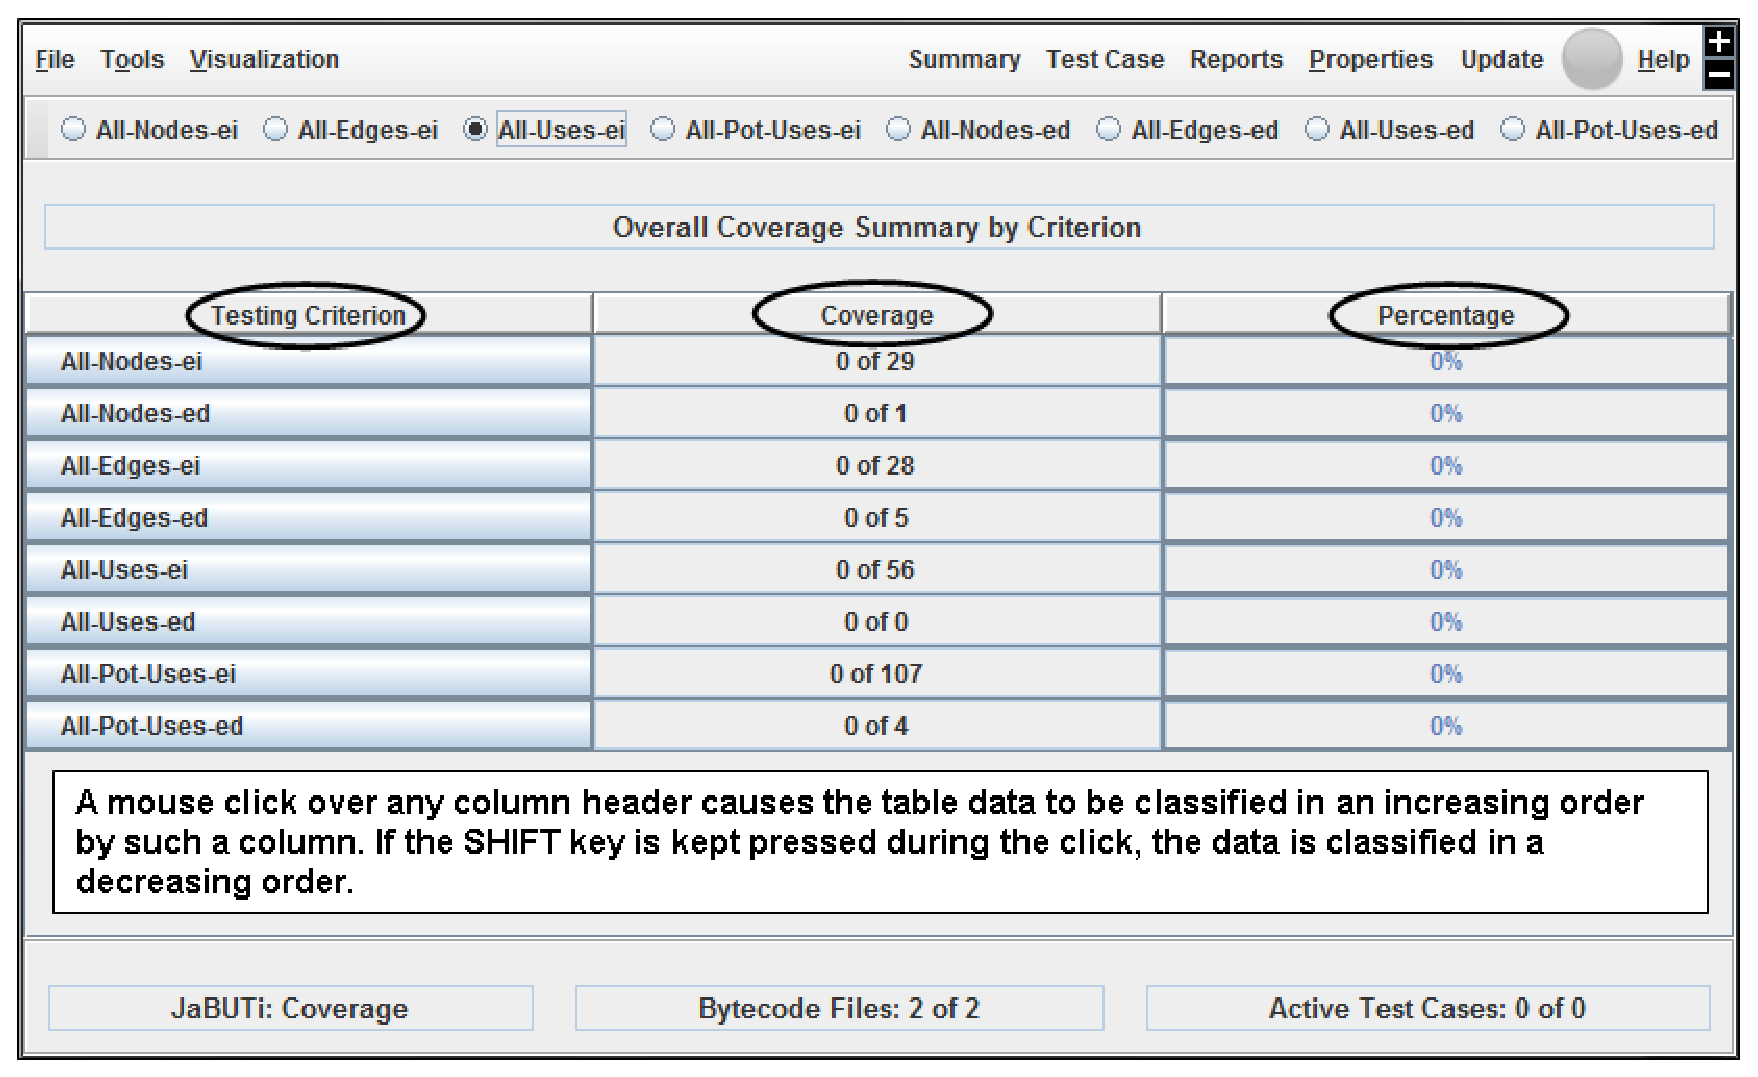
\includegraphics[width=0.70\textwidth]{fig/summary-by-criterion-initial-edited.eps}
\caption{\label{fig:initial-summary-criterion} Initial summary
information per testing criterion.}
\end{center}
\end{figure}


For example, in Figures~\ref{fig:initial-summary-criterion} it is
possible to evaluate the number of required elements by criterion
that were generated for the entire project, i.e., classes
\pk{VendingMachine} and \pk{Dispenser}. The individual information
per class file can be obtained by generating the summary report by
class (Figures~\ref{fig:initial-summary-class}).

When showing the summary by class or by method, the tester can
choose, among the available testing criteria, which one he/she
wants to evaluate.
Figures~\ref{fig:initial-summary-class-pri-nodes},
\ref{fig:initial-summary-class-pri-edges},
and~\ref{fig:initial-summary-class-pri-uses} illustrate the
summary per individual class \wrt the \pk{All-Nodes-ei},
\pk{All-Edges-ei}, and \pk{All-Uses-ei} criteria, respectively.
Considering the summary by class and by method, by clicking on the
class file name or in the method name, the corresponding bytecode
is highlighted and displayed considering the weight \wrt the
selected criterion.

As commented in Figures~\ref{fig:initial-summary-criterion},
double-clicking on the desired column header, any tabled report
generated by \toolname is classified in an increasing order,
considering the clicked column header. A double-click with the
\pk{SHIFT} key pressed causes the table data to be sorted in a
decreasing order.

Using these summary reports the tester can evaluate the current
coverage of each class under testing with different granularity
and decides whether a given class requires additional testing \wrt
six different intra-method testing criteria.
Section~\ref{sec:testcase} illustrates how to include test cases
and how to generate testing reports by test case and by test case
paths.

% This is part of the Jabuti 1.0 Manual.
% Copyright 2003 (c) Auri Marcelo Rizzo Vicenzi, Marcio Eduardo Delamaro,
% Jose Carlos Maldonado.
% See the file FDL.TXT for copying conditions.

\begin{figure}[!ht]
\begin{center}
\subfigure[]{\label{fig:initial-summary-class-pri-nodes}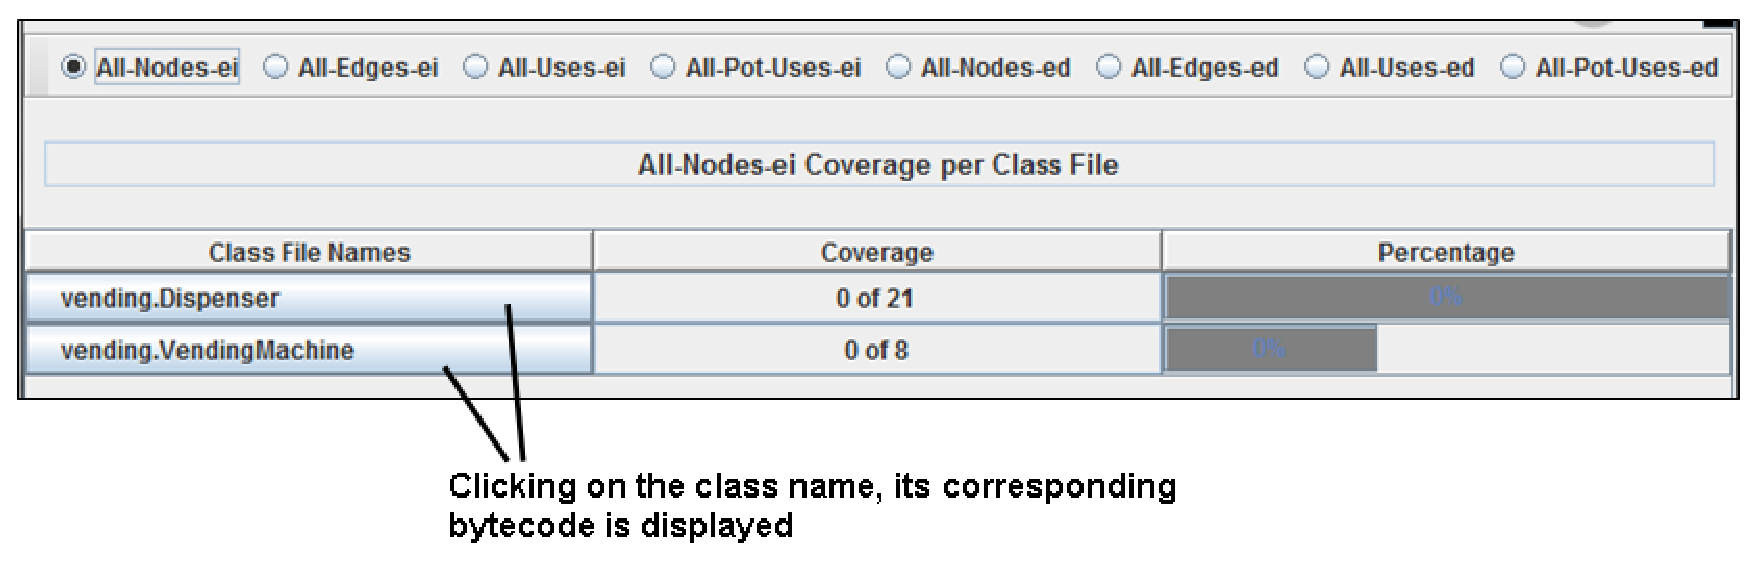
\includegraphics[width=0.70\textwidth]{fig/summary-by-class-pri-nodes-edited.eps}}

\subfigure[]{\label{fig:initial-summary-class-pri-edges}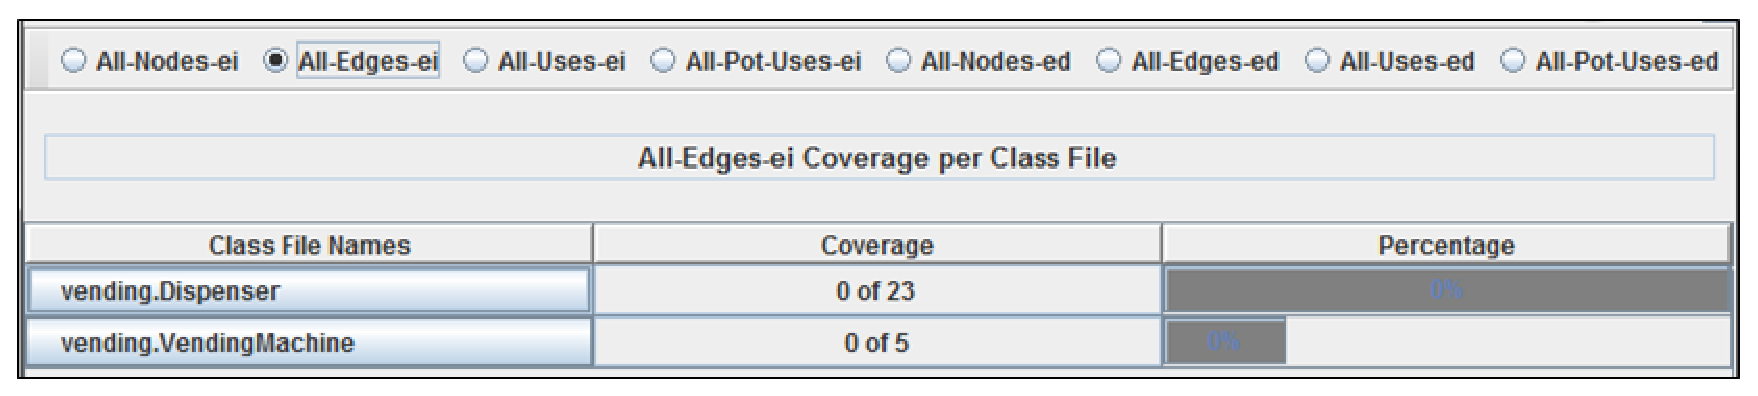
\includegraphics[width=0.70\textwidth]{fig/summary-by-class-pri-edges-edited.eps}}

\subfigure[]{\label{fig:initial-summary-class-pri-uses}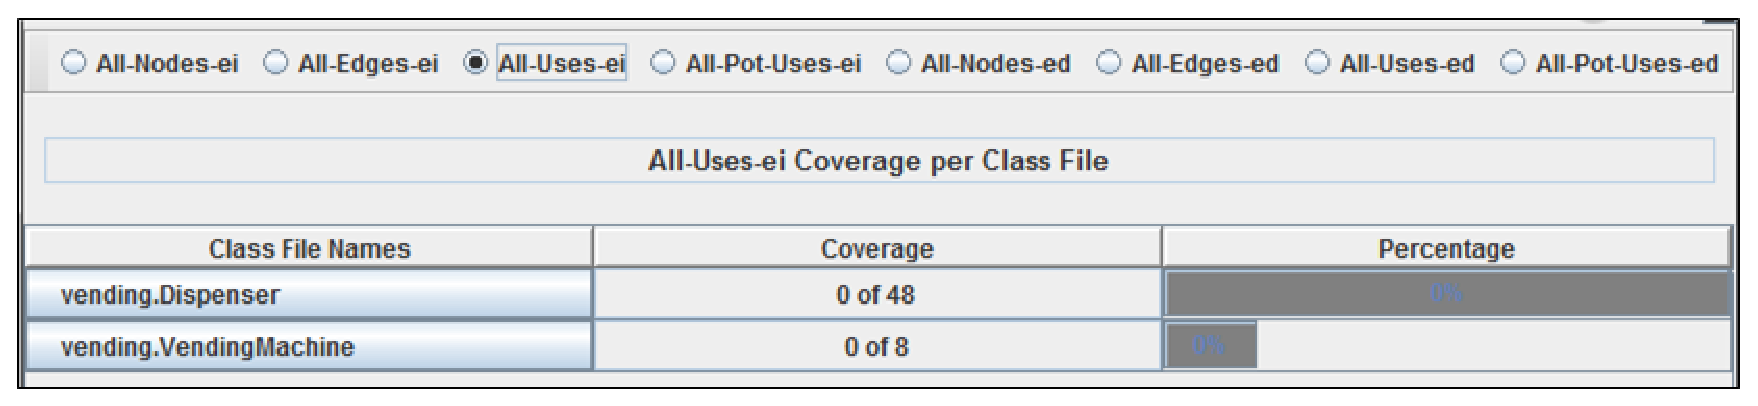
\includegraphics[width=0.70\textwidth]{fig/summary-by-class-pri-uses-edited.eps}}

\caption{Initial summary per class file: (a) \pk{All-Pri-Nodes}
criterion, (b) \pk{All-Pri-Edges} criterion, and (c)
\pk{All-Pri-Uses} criterion.}\label{fig:initial-summary-class}
\end{center}
\end{figure}


% This is part of the Jabuti 1.0 Manual.
% Copyright 2003 (c) Auri Marcelo Rizzo Vicenzi, Marcio Eduardo Delamaro,
% Jose Carlos Maldonado.
% See the file FDL.TXT for copying conditions.

\begin{figure}[!ht]
\begin{center}
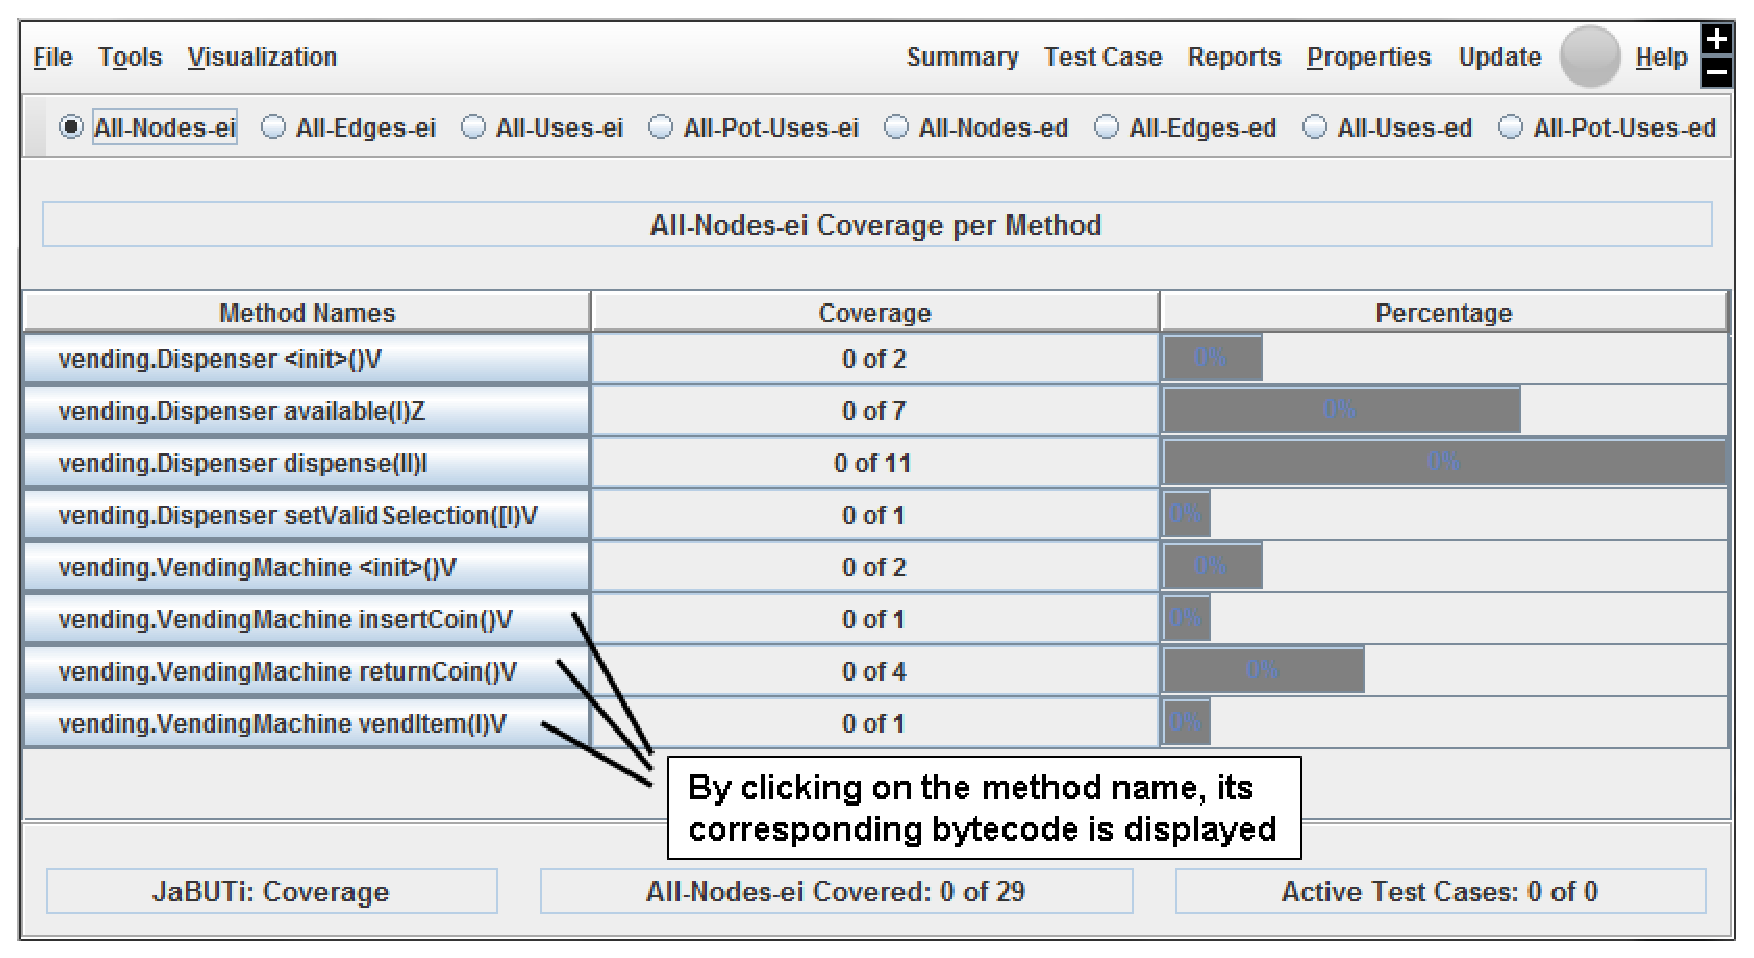
\includegraphics[width=0.70\textwidth]{fig/summary-by-method-initial.eps}
\caption{\label{fig:initial-summary-method} Initial summary
information per method: \pk{All-Pri-Nodes} criterion.}
\end{center}
\end{figure}


\afterpage{\clearpage}
\newpage

\subsection{How to generate an HTML version of a \toolname
report}

As mentioned above, any kind of tabled report presented in
\toolname's graphical interface can be saved as an HTML file
through the \pk{Reports $\rightarrow$ Summary to HTML} menu
option. For example, Figure~\ref{fig:summary-to-html} shows how to
create a \pk{summary-by-criterion.html} file, corresponding to the
current \toolname screen. Figure~\ref{fig:html-file} illustrates
the generated HTML file in a browser window. In this way the
tester can collect and save different testing report showing the
evolution of the testing activity.

% This is part of the Jabuti 1.0 Manual.
% Copyright 2003 (c) Auri Marcelo Rizzo Vicenzi, Marcio Eduardo Delamaro,
% Jose Carlos Maldonado.
% See the file FDL.TXT for copying conditions.

\begin{figure}[!ht]
\begin{center}
\subfigure[]{\label{fig:summary-to-html}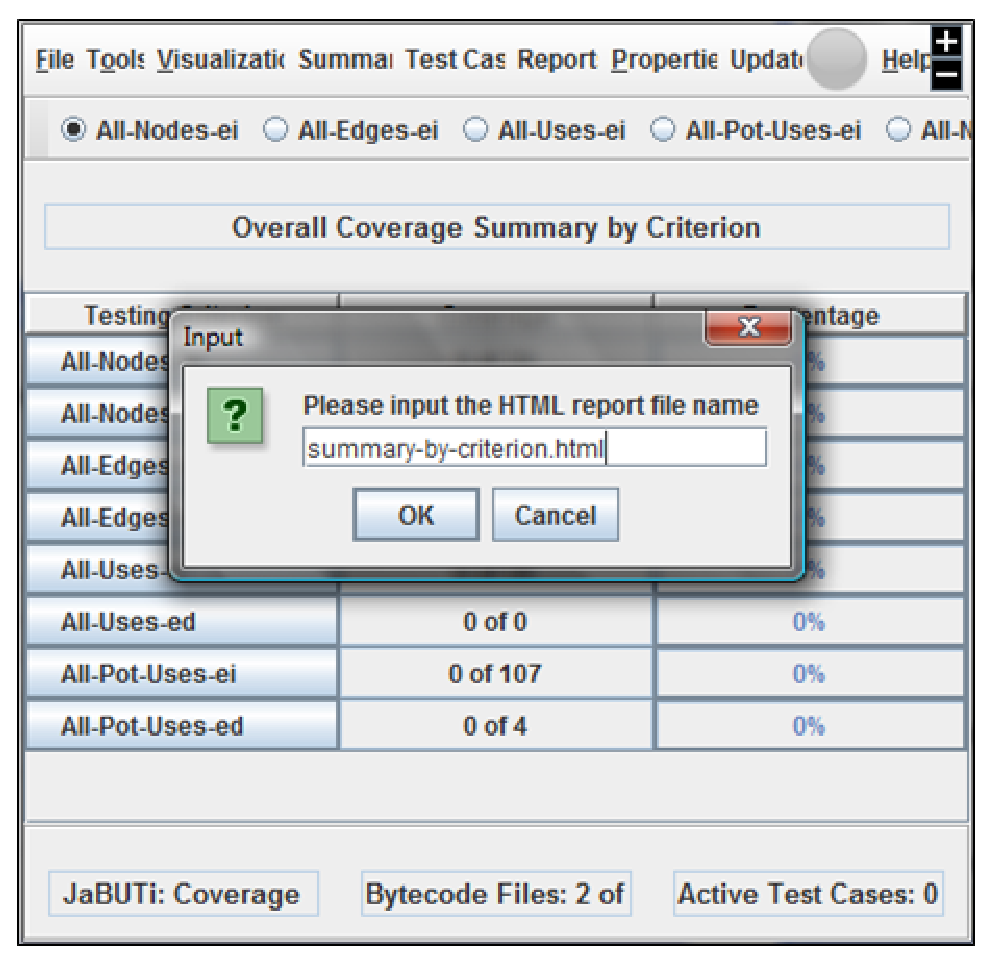
\includegraphics[width=0.45\textwidth]{fig/summary-to-html.eps}}\qquad
\subfigure[]{\label{fig:html-file}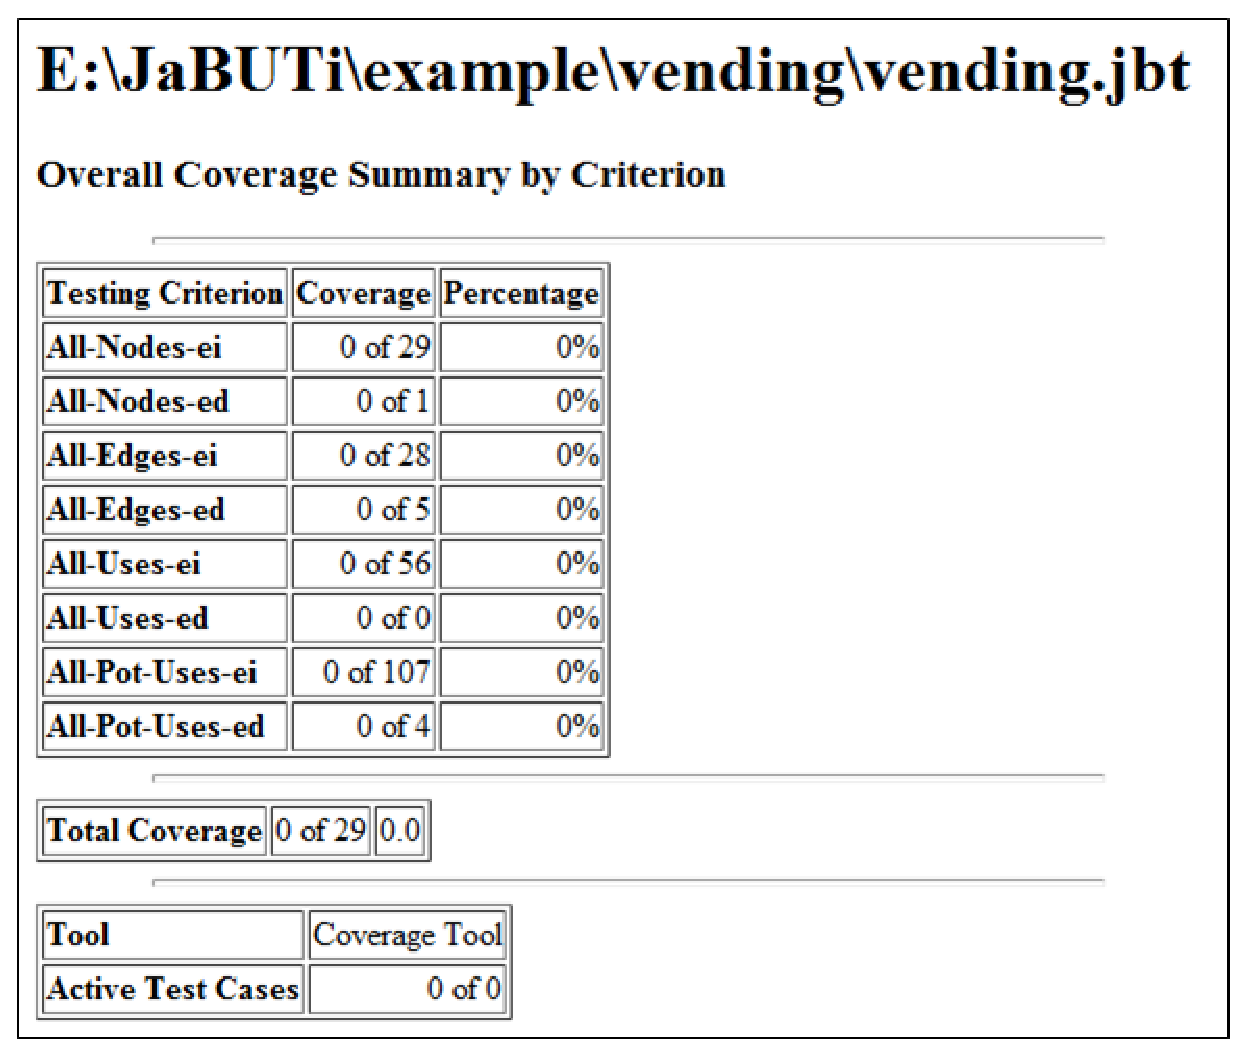
\includegraphics[width=0.45\textwidth]{fig/summary-by-criterion-html.eps}}
\caption{Example of an HTML report generated by
\toolname.}\label{fig:html-report}
\end{center}
\end{figure}


A different kind of report can be generated through the
\pk{Reports $\rightarrow$ Custom Report} menu option. By selecting
this option, a dialog windows, as illustrated in
Figure~\ref{fig:custom-html}, appears and the tester can choose
the level of information that will be saved in a HTML file.
Observe that to save information at method level it is also
required to save information about the class and project level,
since the information is saved hierarchically. Part of a complete
report for the entire project is presented in
Figure~\ref{fig:html-file2}.

% This is part of the Jabuti 1.0 Manual.
% Copyright 2003 (c) Auri Marcelo Rizzo Vicenzi, Marcio Eduardo Delamaro,
% Jose Carlos Maldonado.
% See the file FDL.TXT for copying conditions.

\begin{figure}[!ht]
\begin{center}
\subfigure[]{\label{fig:custom-html}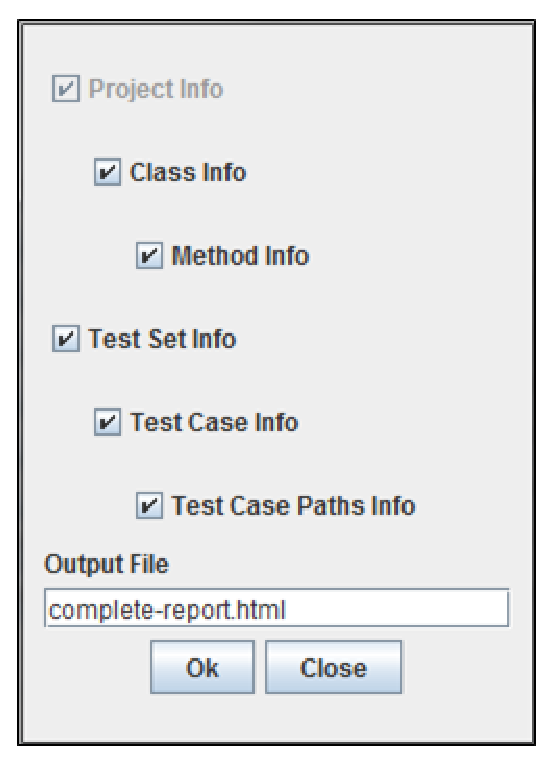
\includegraphics[width=0.25\textwidth]{fig/custom-html.eps}}\qquad
\subfigure[]{\label{fig:html-file2}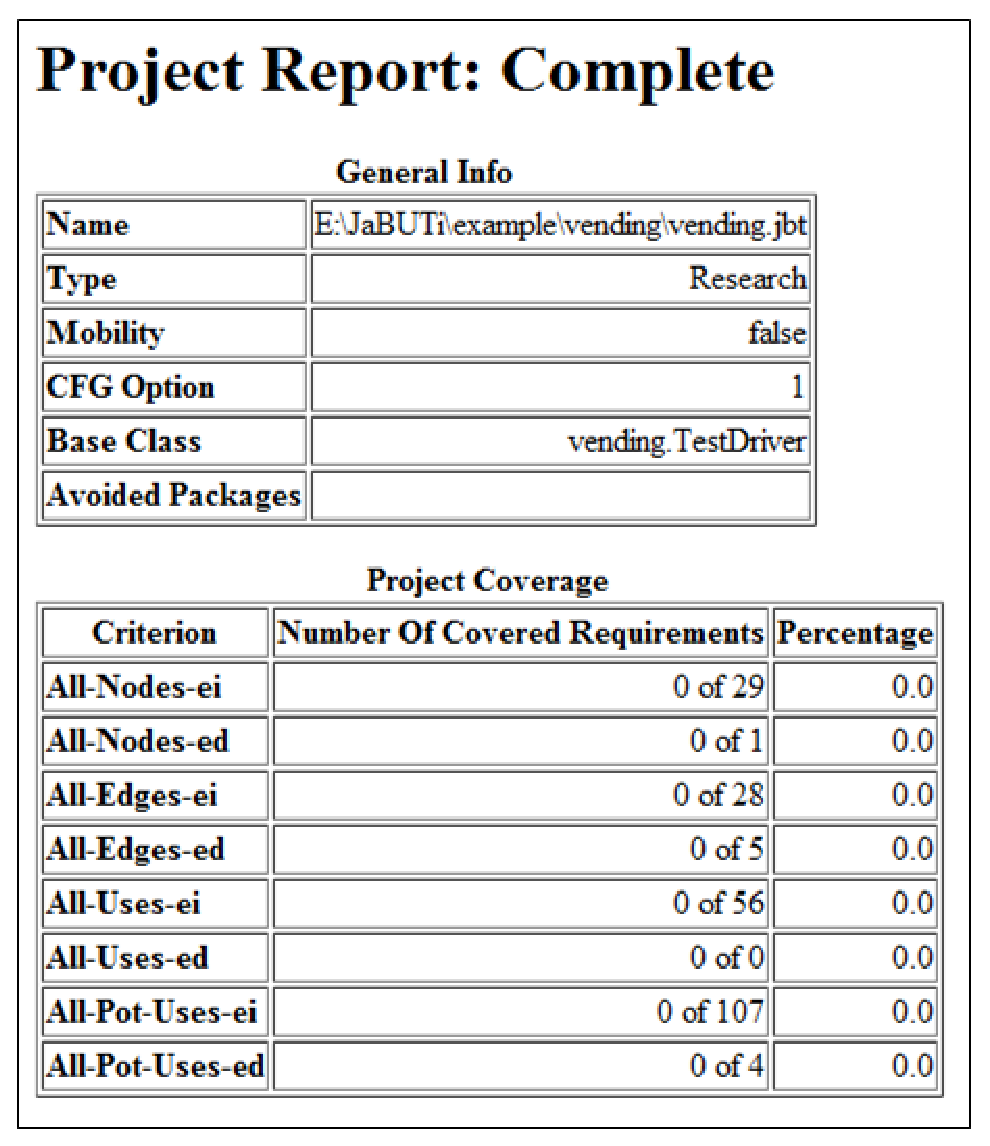
\includegraphics[width=0.45\textwidth]{fig/complete-html.eps}}
\caption{Example of custom HTML report generated by \toolname for
the entire project.}\label{fig:custom-html-report}
\end{center}
\end{figure}


\afterpage{\clearpage}
\newpage

\subsection{How to include a test case}\label{sec:testcase}

\toolname is designed to support test case set adequacy evaluation
and to provide guidance in test case selection. If there is a
previously developed test set, \eg a functional test set, such a
test set can be evaluated against the structural testing criteria
implemented by \toolname. This allows the tester to check, for
example, whether all instructions/statements are executed by a
particular test set. If they are not yet executed, additional test
cases can be developed to improve the quality of the previous test
set.

On the other hand, if there is no previous test set available, the
tester can use the hints provided by the tool to create test cases
aiming at to cover the different testing requirements generated by
\toolname based on its structural criteria. Once the test criteria
can be applied incrementally, the tester can start by developing
an adequate test set \wrt the \pk{All-Nodes-ei} criterion, then,
if necessary, to develop additional test cases to evolve the
\pk{All-Nodes-ei}-adequate test set to a
\pk{All-Edges-ei}-adequate test set, and later, if necessary, to
develop additional test cases to evolve it to an
\pk{All-Uses-ei}-adequate test set. All these criteria, prefixed
by \pk{All-Pri-}, are related with the normal program execution.
If desired, the tester can check the coverage of the
exception-handling mechanism, by using the \pk{All-Nodes-ed},
\pk{All-Edges-ed} and \pk{All-Uses-ed} criteria. The idea is to
use these criteria incrementally to reduce their complexity and
also to allow the tester to deal with the cost and time
constraints.

\begin{sloppypar}
\toolname allows to include test cases in two different ways: 1)
using the \toolname's class loader; or 2) importing from a JUnit
test set. The first is done by a command line application
(\pk{probe.ProberLoader}, the \toolname's class loader). This
command line application extends the default Java class
loader~\cite{Lindholm99JVMS} such that, from a given testing
project, it identifies which classes should be instrumented before
to be loaded and executed. By detecting that a given class belongs
to the set of classes under testing, \toolname's class loader
inserts the probes to collect the execution trace and then loads
the instrumented class file to be executed. The trace information
\wrt the current execution is appended in a trace file with the
same name of the testing project but with the extension \trcext
instead of \prjext.
\end{sloppypar}

For example, the test case file \pk{input1}, presented in
Figure~\ref{fig:input1}, touches the testing requirement
(considering the \pk{All-Nodes-ei} criterion) with the highest
weight illustrated in Figure~\ref{fig:dispenser-source} and also
reveals a fault contained in the \pk{Dispenser} component. Such a
test case will be used in the next section to show how to use
\toolname to ease the fault localization.

\begin{figure}[!ht]
\begin{cmd}
auri@AURIMRV ~/example
$ cat input1
insertCoin
vendItem 3
\end{cmd}
\vspace{-0.7cm} \caption{Example of test case
file.}\label{fig:input1}
\end{figure}

The command line in Figure~\ref{fig:driver-output}(a) shows the
output of the \pk{vending.TestDriver} when executed by the default
class loader. Figure~\ref{fig:driver-output}(b) shows the
resultant output when \pk{vending.TestDriver} is executed using
the \toolname's class loader. The execution of the command as
shown in Figure~\ref{fig:driver-output}(b) causes the
\pk{vending\trcext} to be generated/updated with the execution
path of test case file \pk{input1}.

% This is part of the Jabuti 1.0 Manual.
% Copyright 2003 (c) Auri Marcelo Rizzo Vicenzi, Marcio Eduardo Delamaro,
% Jose Carlos Maldonado.
% See the file FDL.TXT for copying conditions.

\begin{figure}[!ht]
\begin{center}\cmdsize
\begin{tabular}{|c|c|}\hline
&\\
\begin{minipage}{2.7in}
\begin{verbatim}
auri@AURIMRV ~/example
$ java -cp "." vending.TestDriver input1
VendingMachine ON
Current value = 25
Enter 25 coins
Current value = -25
VendingMachine OFF







\end{verbatim}
\end{minipage}
&
\begin{minipage}{3.6in}
\begin{verbatim}
auri@AURIMRV ~/example
$ java -cp ".;..\Tools\jabuti;\
>..\Tools\jabuti\lib\BCEL.jar;\
>..\Tools\jabuti\lib\crimson.jar;\
> probe.ProberLoader -P vending.jbt \
> vending.TestDriver input1
Project Name: vending.jbt
Trace File Name: vending.trc
Processing File vending.jbt
VendingMachine ON
Current value = 25
Enter 25 coins
Current value = -25
VendingMachine OFF
\end{verbatim}
\end{minipage}\\
&\\\hline
\multicolumn{1}{c}{(a)} & \multicolumn{1}{c}{(b)}\\
\end{tabular}
\end{center}
\caption{\pk{vending.TestDriver} output: (a) default class loader, and (b)
\toolname class loader.}\label{fig:driver-output}
\end{figure}


Considering Figure~\ref{fig:driver-output}(b), observe that the
\pk{CLASSPATH} variable is set containing all the paths necessary
to run the \toolname's class loader and also the vending machine
example. The next parameter, \pk{probe.ProberLoader}, is the name
of the \toolname's class loader. It demands two parameters to
execute: the name of the project (\pk{-P vending.jbt}), and the
name of the base class to be executed (\pk{vending.TestDriver}).
In our example, since \pk{vending.TestDriver} requires one
parameter to be executed, this parameter is also provided
(\pk{input1}). During the execution of \pk{vending.TestDriver},
\pk{VendingMachine} and \pk{Dispenser} classes are required to be
loaded. From the project file (\pk{vending.jbt}) the \toolname's
class loader detects that these class files have to be
instrumented before to be executed. The instrumentation is
performed on-the-fly every time the \pk{probe.ProberLoader} is
invoked.

The resultant execution trace information, corresponding to the
execution of the test case \pk{input1}, is appended in the end of
the trace file \pk{vending\trcext}. Every time the size of the
trace file increase, the \pk{Update} button in the \toolname's
graphical interface becomes red, indicating that the coverage
information can be updated considering the new test case(s).
Figure~\ref{fig:update-button} illustrates this event.

% This is part of the Jabuti 1.0 Manual.
% Copyright 2003 (c) Auri Marcelo Rizzo Vicenzi, Marcio Eduardo Delamaro,
% Jose Carlos Maldonado.
% See the file FDL.TXT for copying conditions.

\begin{figure}[!ht]
\begin{center}
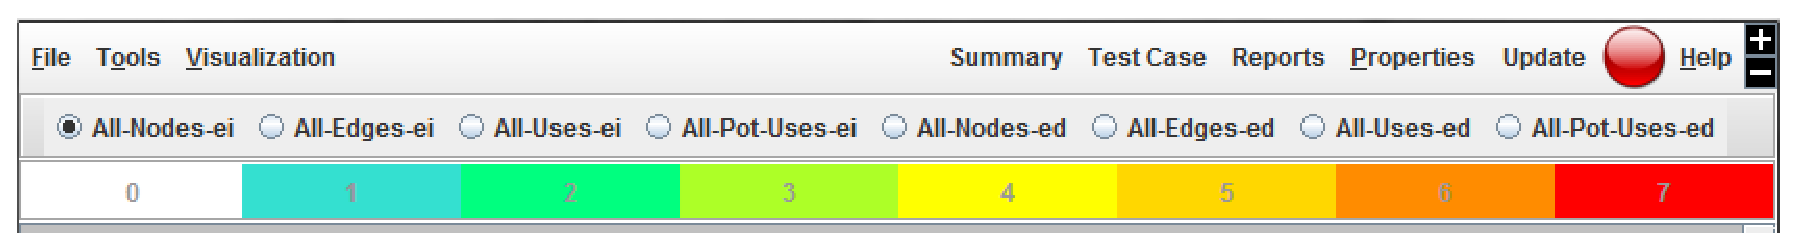
\includegraphics[width=0.70\textwidth]{fig/update-button.eps}
\caption{\label{fig:update-button} Update button with a different
background color: new test case(s) available.}
\end{center}
\end{figure}


By clicking on the \pk{Update} button, \toolname imports the new
test case(s), empties the trace file \pk{vending\trcext} and
updates the coverage information and the weights for each testing
criterion. For example, after the importation of test case
\pk{input1}, the weight of the Java source code \wrt the
All-Nodes-ei criterion changed as illustrated in
Figure~\ref{fig:source-input1}.

% This is part of the Jabuti 1.0 Manual.
% Copyright 2003 (c) Auri Marcelo Rizzo Vicenzi, Marcio Eduardo Delamaro,
% Jose Carlos Maldonado.
% See the file FDL.TXT for copying conditions.

\begin{figure}[!ht]
\begin{center}
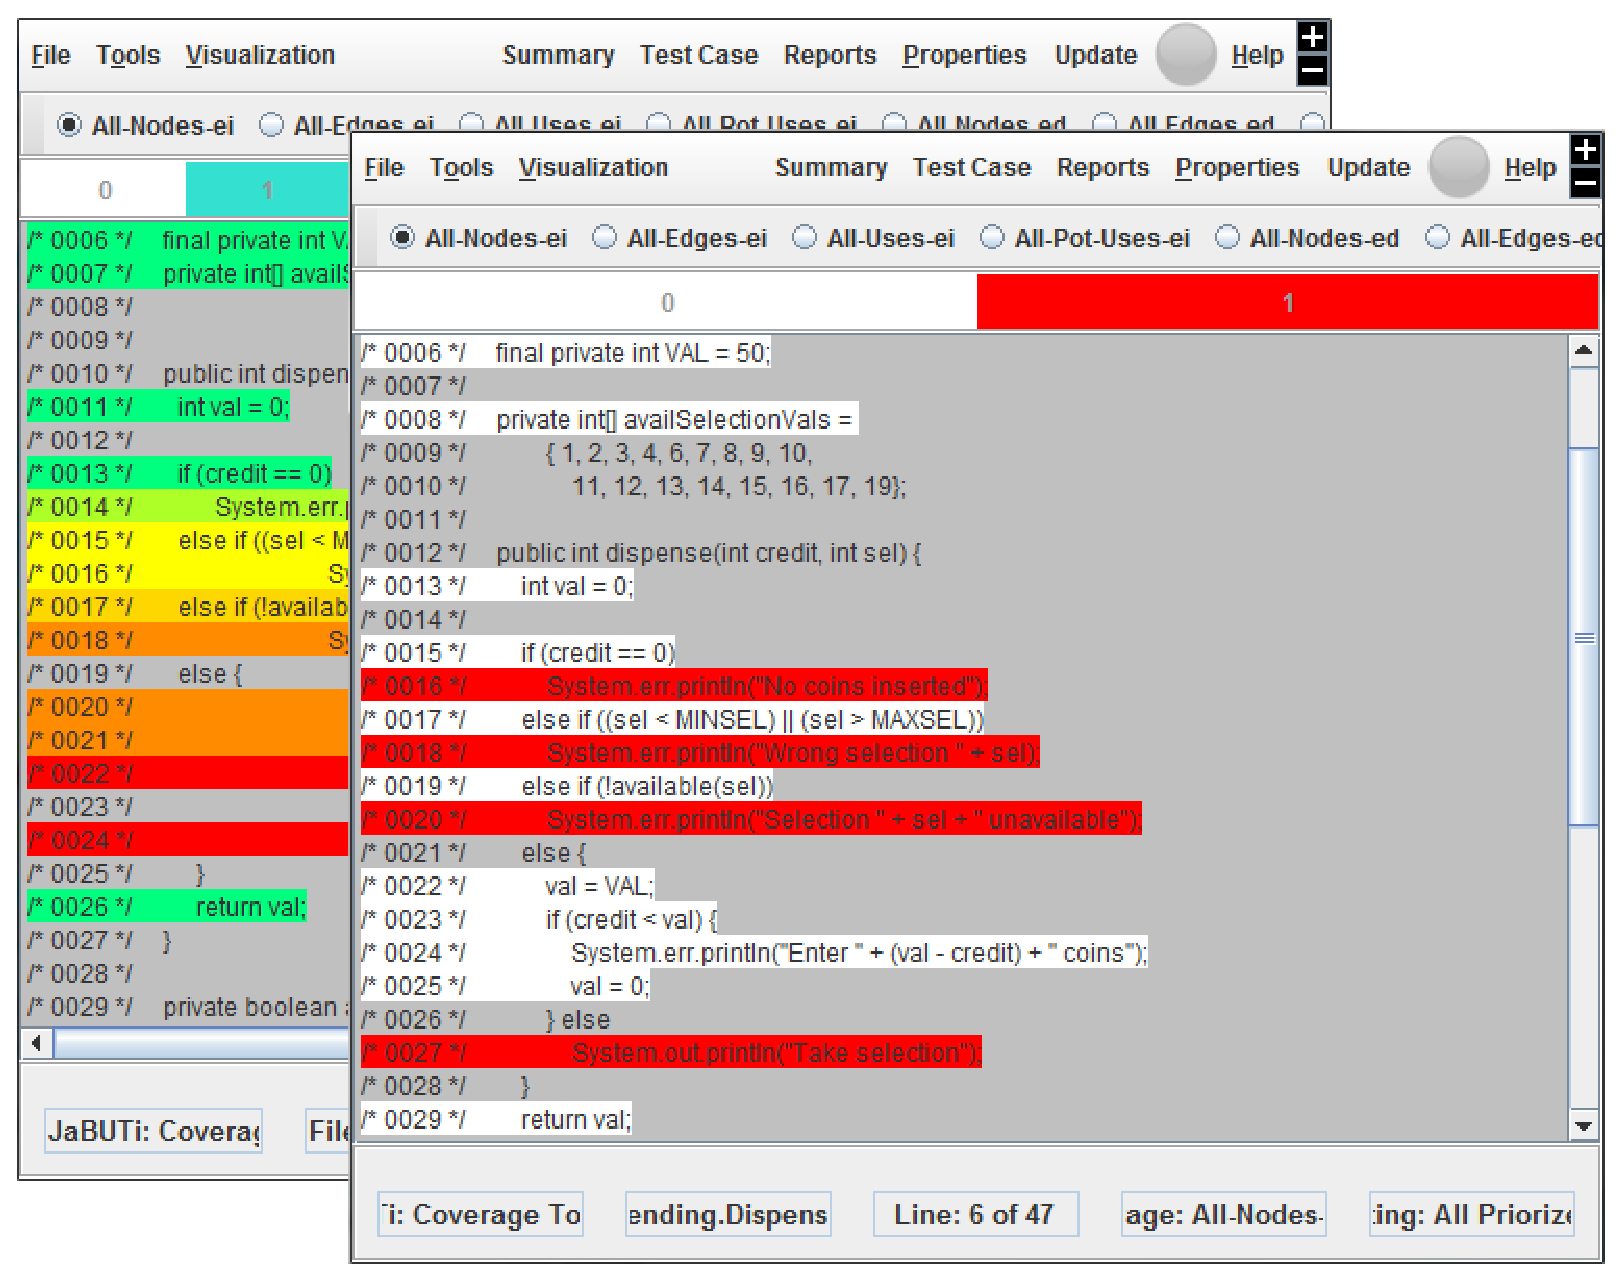
\includegraphics[height=0.40\textheight]{fig/dispenser-source-edited.eps}
\caption{\label{fig:source-input1} \pk{Dispenser.dispenser()}
method before and after the weight's updating \wrt
\pk{All-Pri-Nodes} criterion.}
\end{center}
\end{figure}


Comparing the updated source of Figure~\ref{fig:source-input1}
(front) with the one presented in Figure~\ref{fig:source-input1}
(back) it can be observed that the requirement with the highest
changed from source lines 22 and 24 (now covered -- painted in white) to
source lines 16, 18, 20 and 27. Considering the entire project,
Figure~\ref{fig:summary-method-tc1} shows the updated coverage for
each method in the \pk{Dispenser} and \pk{VendingMachine} classes
\wrt the \pk{All-Nodes-ei} criterion. Observe that \pk{input1}
covered 7 primary nodes (63\%) of \pk{Dispenser.dispense} method
and 19 of 29 primary nodes (65\%) considering the entire project.
By accessing the \pk{Test Case $\rightarrow$ Report by Test Case}
menu option, the tester can visualize the coverage of the entire
project by test case, as illustrated in
Figure~\ref{fig:report_tc1}.

% This is part of the Jabuti 1.0 Manual.
% Copyright 2003 (c) Auri Marcelo Rizzo Vicenzi, Marcio Eduardo Delamaro,
% Jose Carlos Maldonado.
% See the file FDL.TXT for copying conditions.

\begin{figure}[!ht]
\begin{center}
\subfigure[Report by test
case]{\label{fig:report_tc1}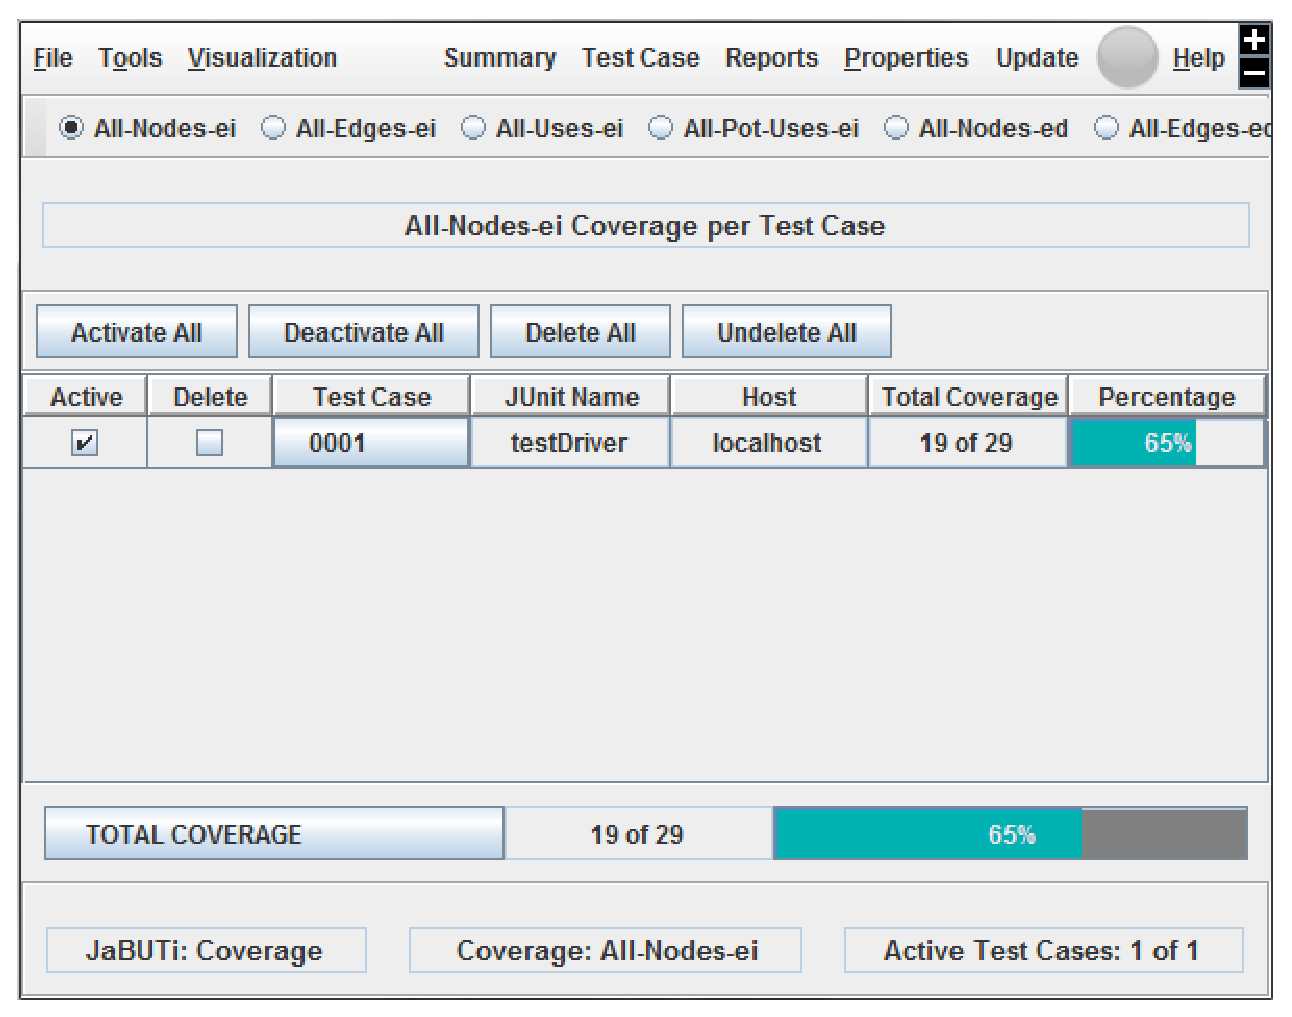
\includegraphics[width=0.40\textwidth]{fig/report-by-test-case-tc1.eps}}\qquad
\subfigure[Summary by
Method]{\label{fig:summary-method-tc1}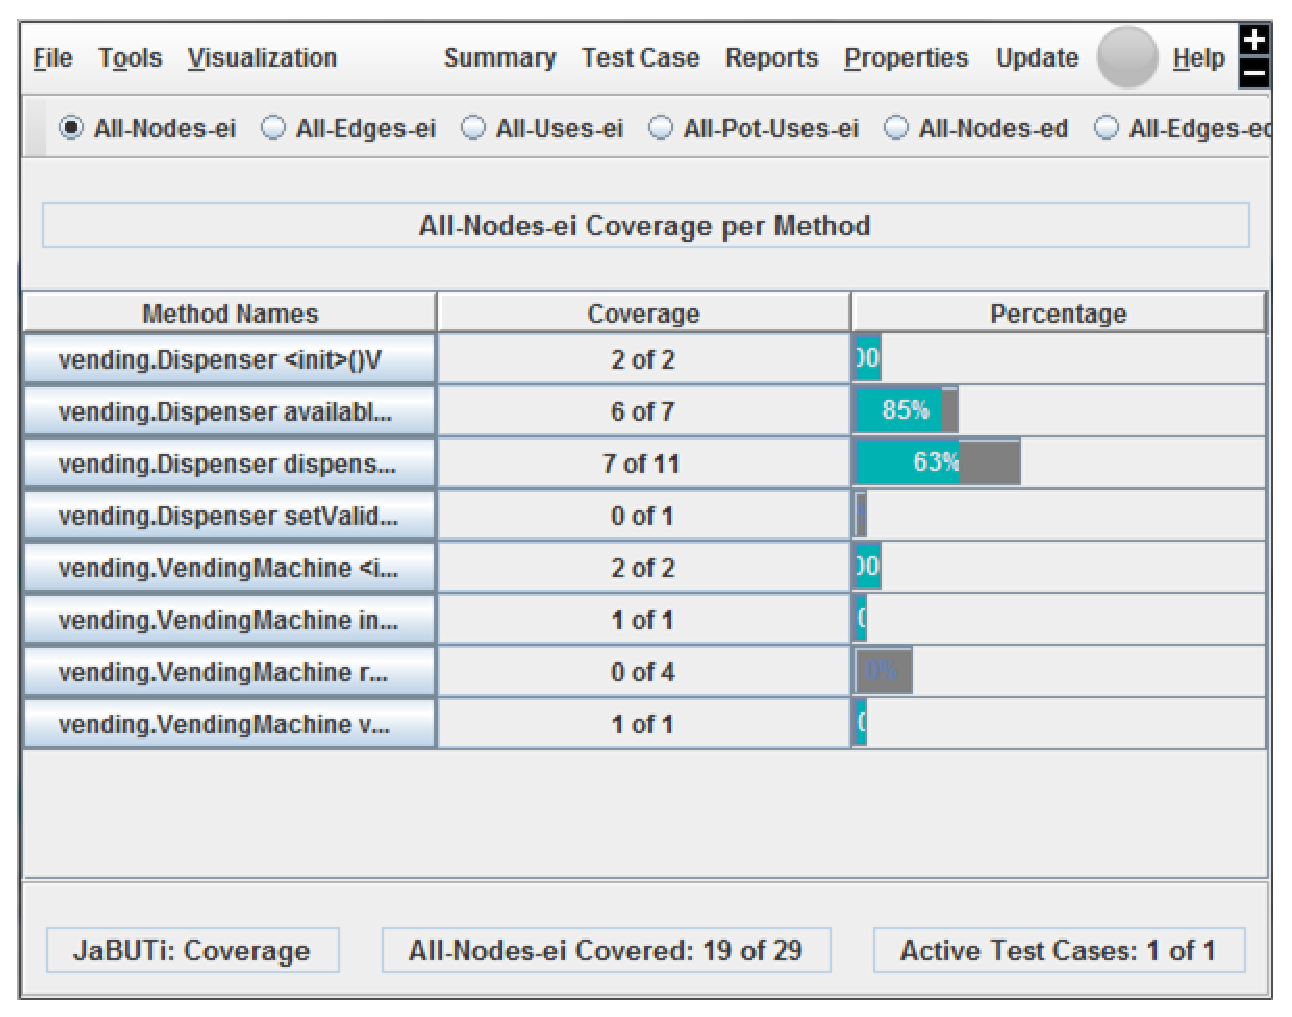
\includegraphics[width=0.50\textwidth]{fig/summary-by-method-tc1.eps}}
\caption{Updated coverage after test case
\pk{input1}.}\label{fig:tc1}
\end{center}
\end{figure}


If desired, the tester can develop additional test cases to
improve the coverage \wrt \pk{All-Nodes-ei} criterion. For
example, besides \pk{input1}, Table~\ref{tab:adequate} shows four
additional test cases developed to improve the coverage of such a
criterion.

\begin{table}[!ht]
\caption{Adequate test set to the \pk{Dispenser}
component.}\label{tab:adequate}
\begin{center}
\begin{tabular}{|l|l|l|}\hline
\textbf{Name} & \textbf{Content} & \textbf{Correct output}\\
\hline
input1  &   insertCoin      & no  \\
        &   vendItem 3      &     \\ \hline
input2  &   insertCoin      & yes \\
        &   vendItem 18     &     \\ \hline
input3  &   insertCoin      & yes \\
        &   insertCoin      &     \\
        &   vendItem 25     &     \\ \hline
input4  &   vendItem 3      & yes \\ \hline
input5  &   insertCoin      & yes \\
        &   insertCoin      &     \\
        &   vendItem 3      &     \\ \hline
\end{tabular}
\end{center}
\end{table}

%\begin{sloppypar}
%\toolname also allows to visualize the coverage of a given test
%case by each execution path (\pk{Test Case $\rightarrow$ Report by
%Test Case Path}), i.e., during the execution of a single test
%case, several methods can be executed, and each one can be
%executed several times. Each method execution is considered as a
%different execution path. Therefore, a test case is composed by
%zero or more test paths, one for each individual method execution.
%Figure~\ref{fig:report-by-test-path} shows this kind of report.
%For instance, test case \pk{0001} is composed by six paths
%numbered from \pk{0001-0} to \pk{0001-5}. Besides the coverage by
%path, the report also shows additional information about each
%path, collected during the execution.
%\end{sloppypar}
%
%% This is part of the Jabuti 1.0 Manual.
% Copyright 2003 (c) Auri Marcelo Rizzo Vicenzi, Marcio Eduardo Delamaro,
% Jose Carlos Maldonado.
% See the file FDL.TXT for copying conditions.

\begin{figure}[!ht]
\begin{center}
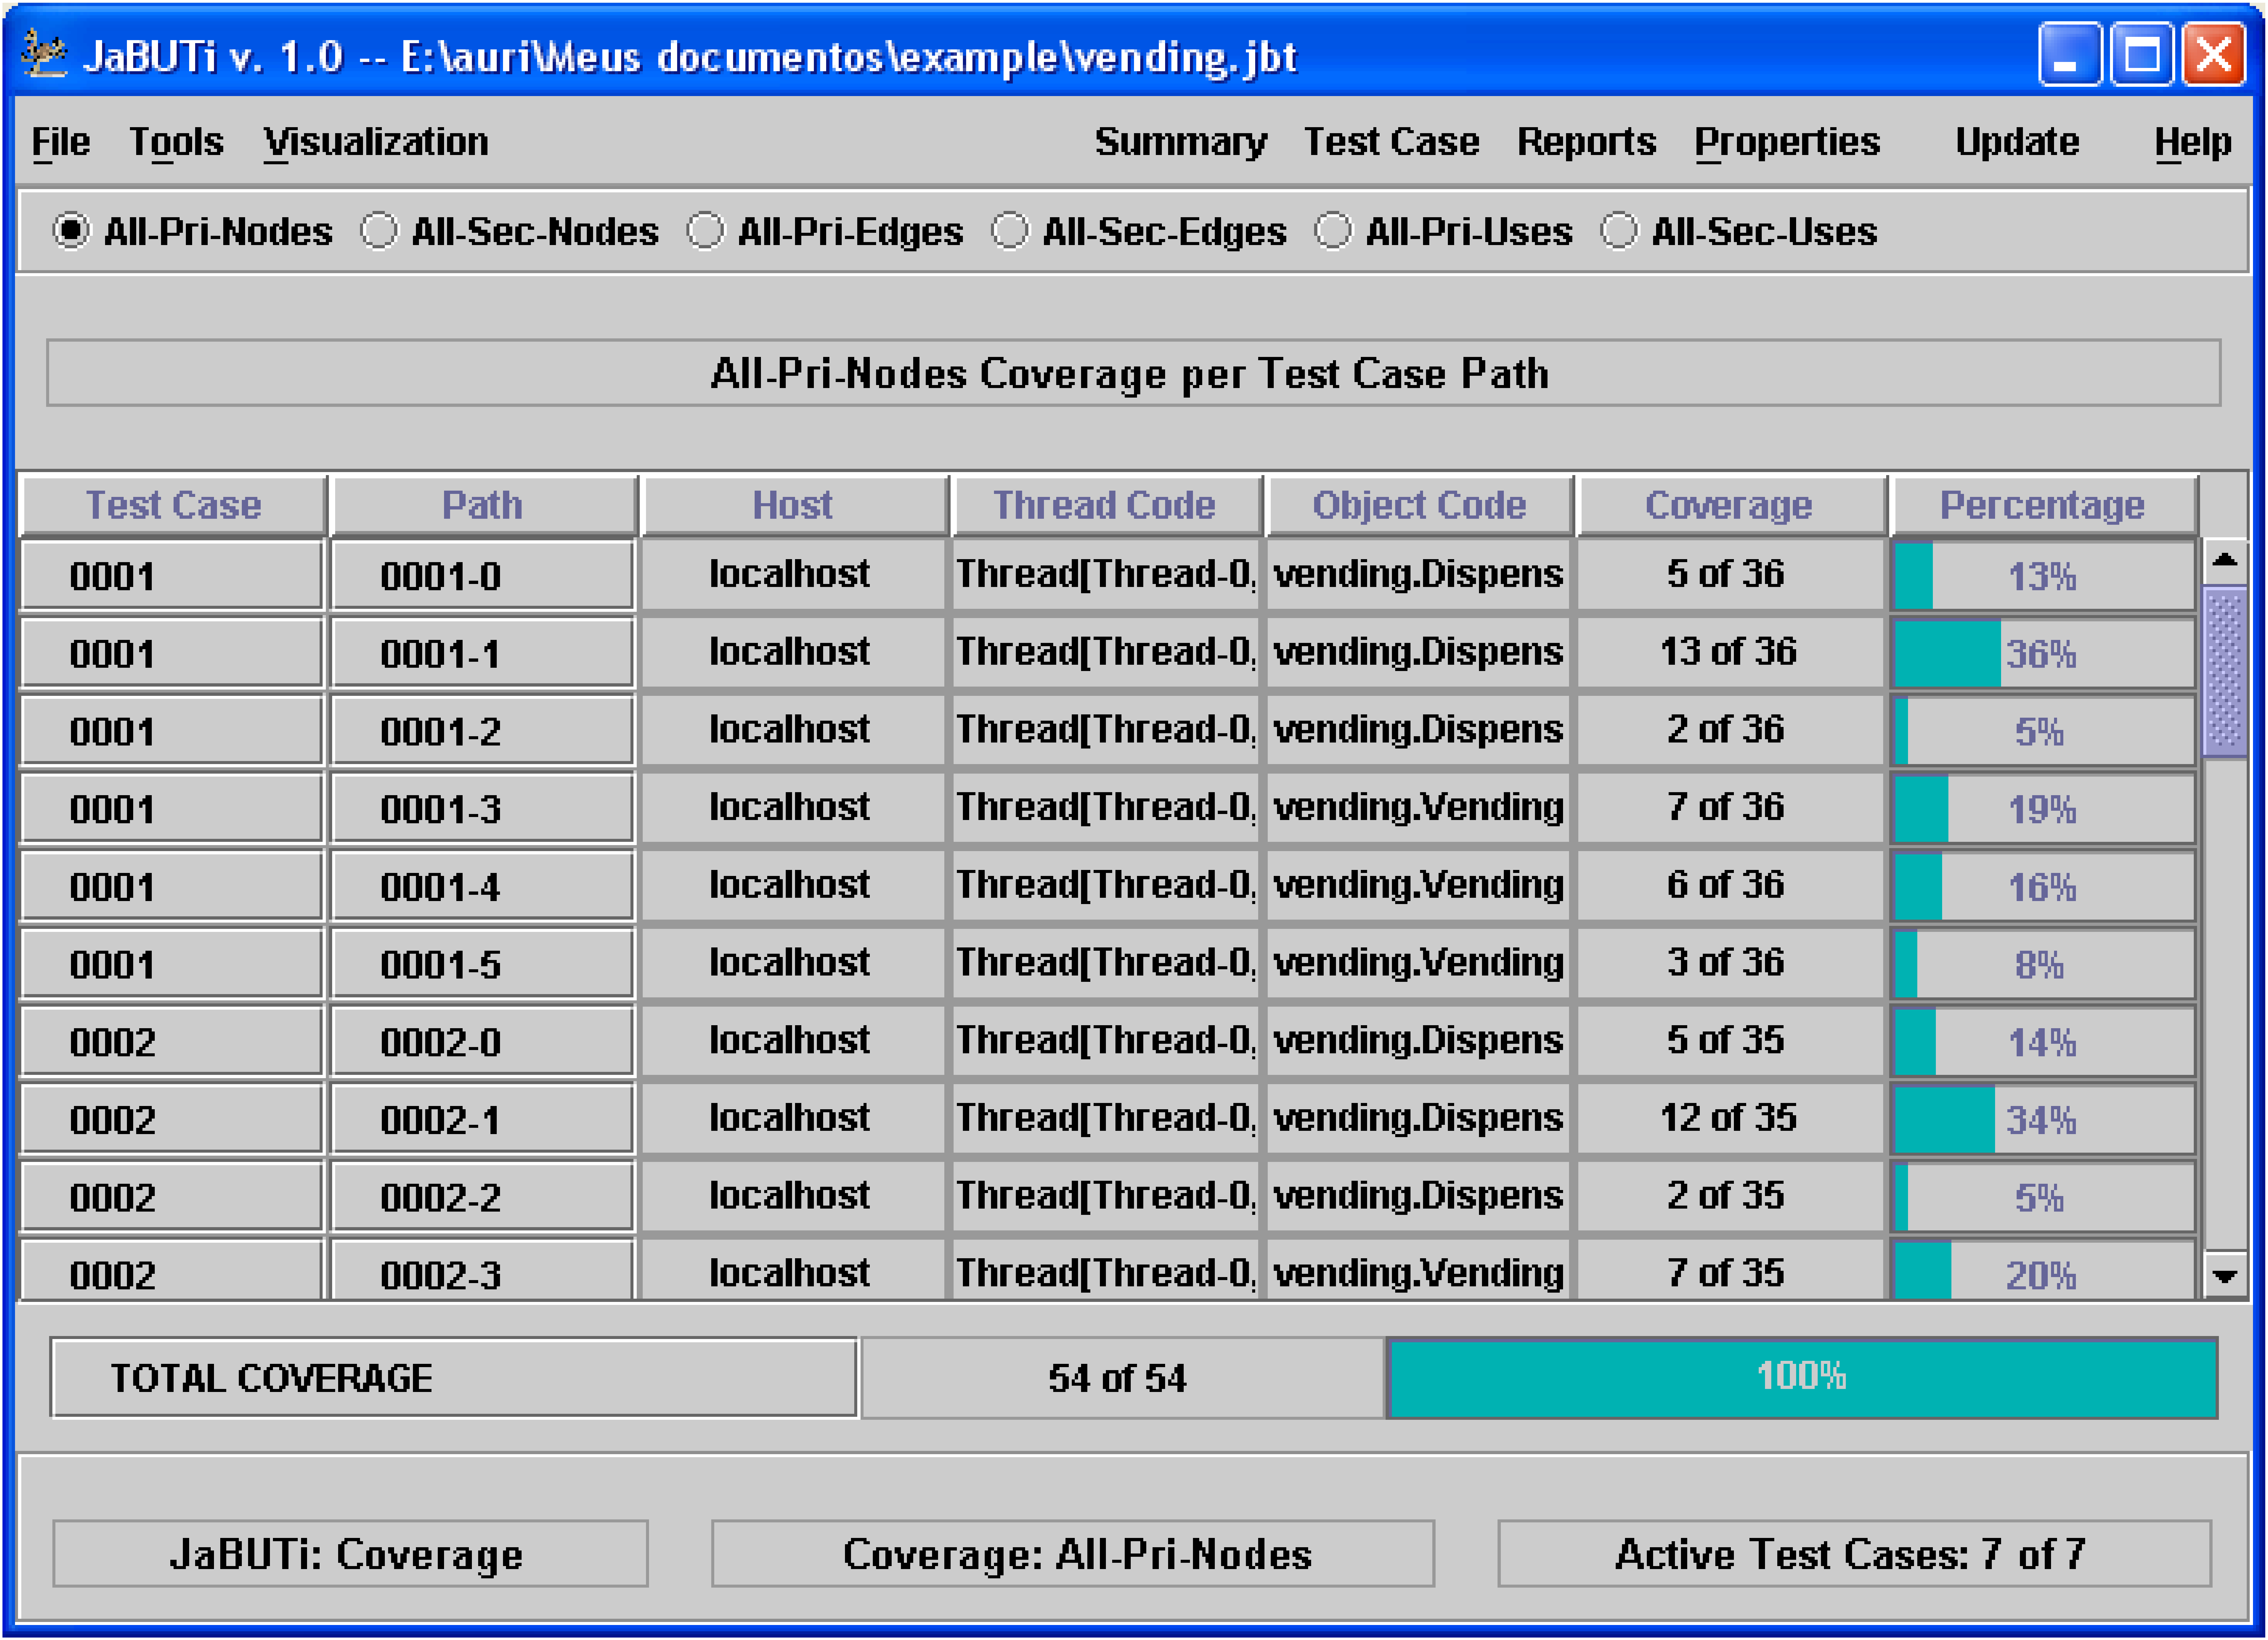
\includegraphics[width=0.70\textwidth]{fig/report-by-test-path.eps}
\caption{\label{fig:report-by-test-path} Testing report by
execution path \wrt the \pk{All-Pri-Nodes} criterion.}
\end{center}
\end{figure}


\afterpage{\clearpage}
\newpage

\subsection{How to import test cases from JUnit framework}

Observe that after five test cases, the coverage of almost all
methods, \wrt the \pk{All-Nodes-ei} criterion, is 100\%. The only
two methods uncovered are \pk{Dispenser.setValidSelection()} and
\pk{VendingMachine.returnCoin()}. To obtain a adequate test set
\wrt the \pk{All-Nodes-ei}, additional test cases are required.
Figure~\ref{fig:junit} shows one additional test case, specified
according to the JUnit framework, to cover 100\% of required
elements of the \pk{All-Nodes-ei} for the \pk{Dispenser} class.
More information about how to develop test set using the JUnit
framework can be found
elsewhere~\cite{JUnit02UDCA,Rainsberger03JSGU}.

% This is part of the Jabuti 1.0 Manual.
% Copyright 2003 (c) Auri Marcelo Rizzo Vicenzi, Marcio Eduardo Delamaro,
% Jose Carlos Maldonado.
% See the file FDL.TXT for copying conditions.

\begin{figure}[!ht]
\begin{center}
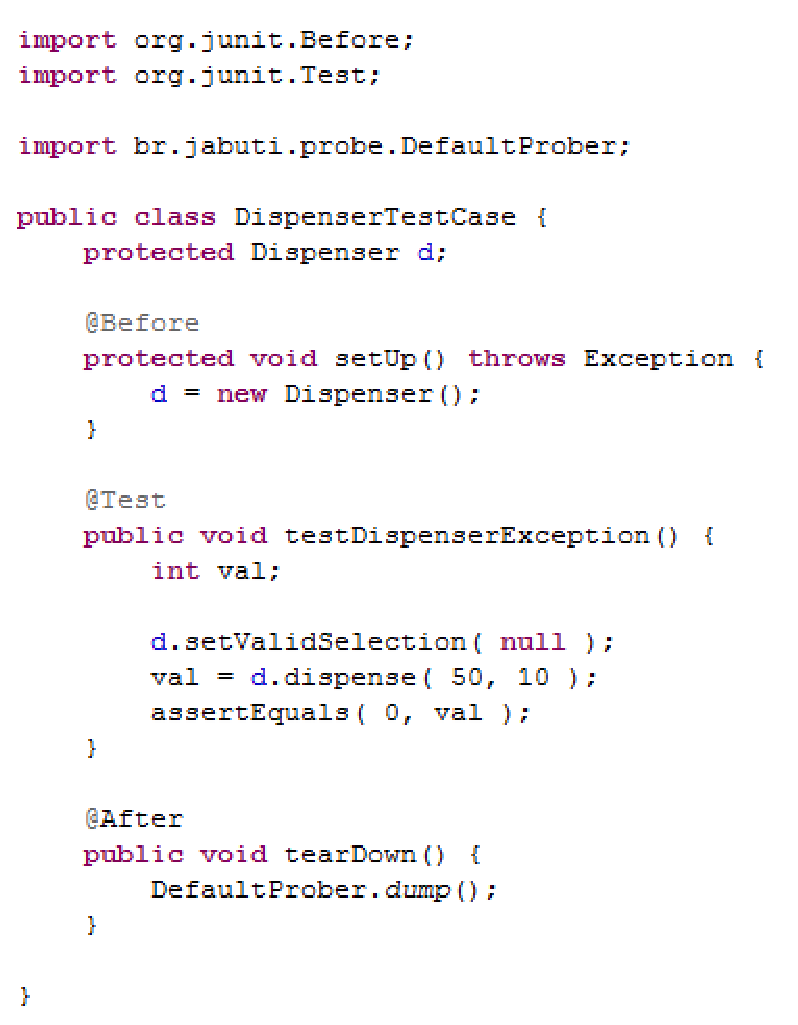
\includegraphics[width=0.4\textwidth]{fig/junit-test-case.eps}
\caption{\label{fig:junit}Example of a test set using the JUnit
framework.}
\end{center}
\end{figure}


As can be observed in Figure~\ref{fig:junit}, 
%line 26, 
\toolname requires that a static method (\pk{DefaultProber.dump()}) to be
called at the end of each test case
%\footnote{JUnit has two special
%methods \pk{TestCase.setUp()} and \pk{TestCase.tearDown()}. The
%former is executed before any test case execution and the later
%after a test case execution. Therefore, since we want to execute
%the method \pk{DefaultProber.dump()} after the execution of each
%test case, a call to such a method is placed inside the method
%\pk{TestCase.tearDown()}.}. 
Such a method is responsible to write
the execution trace in the trace file. Observe that to call such a
static method it is also necessary to include the import statement
%as shown in line 04. 
for the class. Once compiled, such a JUnit test case can be
imported by \toolname from the \pk{Test Case $\rightarrow$ Import
from JUnit} menu option. Figure~\ref{fig:importing-junit} shows
the screen to import a JUnit's test case.

%\begin{enumerate}
%    \item Click on the \pk{Browser} button
%    (Figure~\ref{fig:junit1});
%
%    \item Select the directory where the JUnit test case class file is located
%    (Figure~\ref{fig:junit2});
%
%    \item Select the JUnit test case class file (\pk{DispenserTestCase.class}
%    -- Figure~\ref{fig:junit3});
%
%    \item Select the test cases to be imported and click on the
%    \pk{Import Selected} button (Figure~\ref{fig:junit4}).
%\end{enumerate}

% This is part of the Jabuti 1.0 Manual.
% Copyright 2003 (c) Auri Marcelo Rizzo Vicenzi, Marcio Eduardo Delamaro,
% Jose Carlos Maldonado.
% See the file FDL.TXT for copying conditions.

\begin{figure}[!ht]
\begin{center}
%\subfigure[]{
\label{fig:junit1}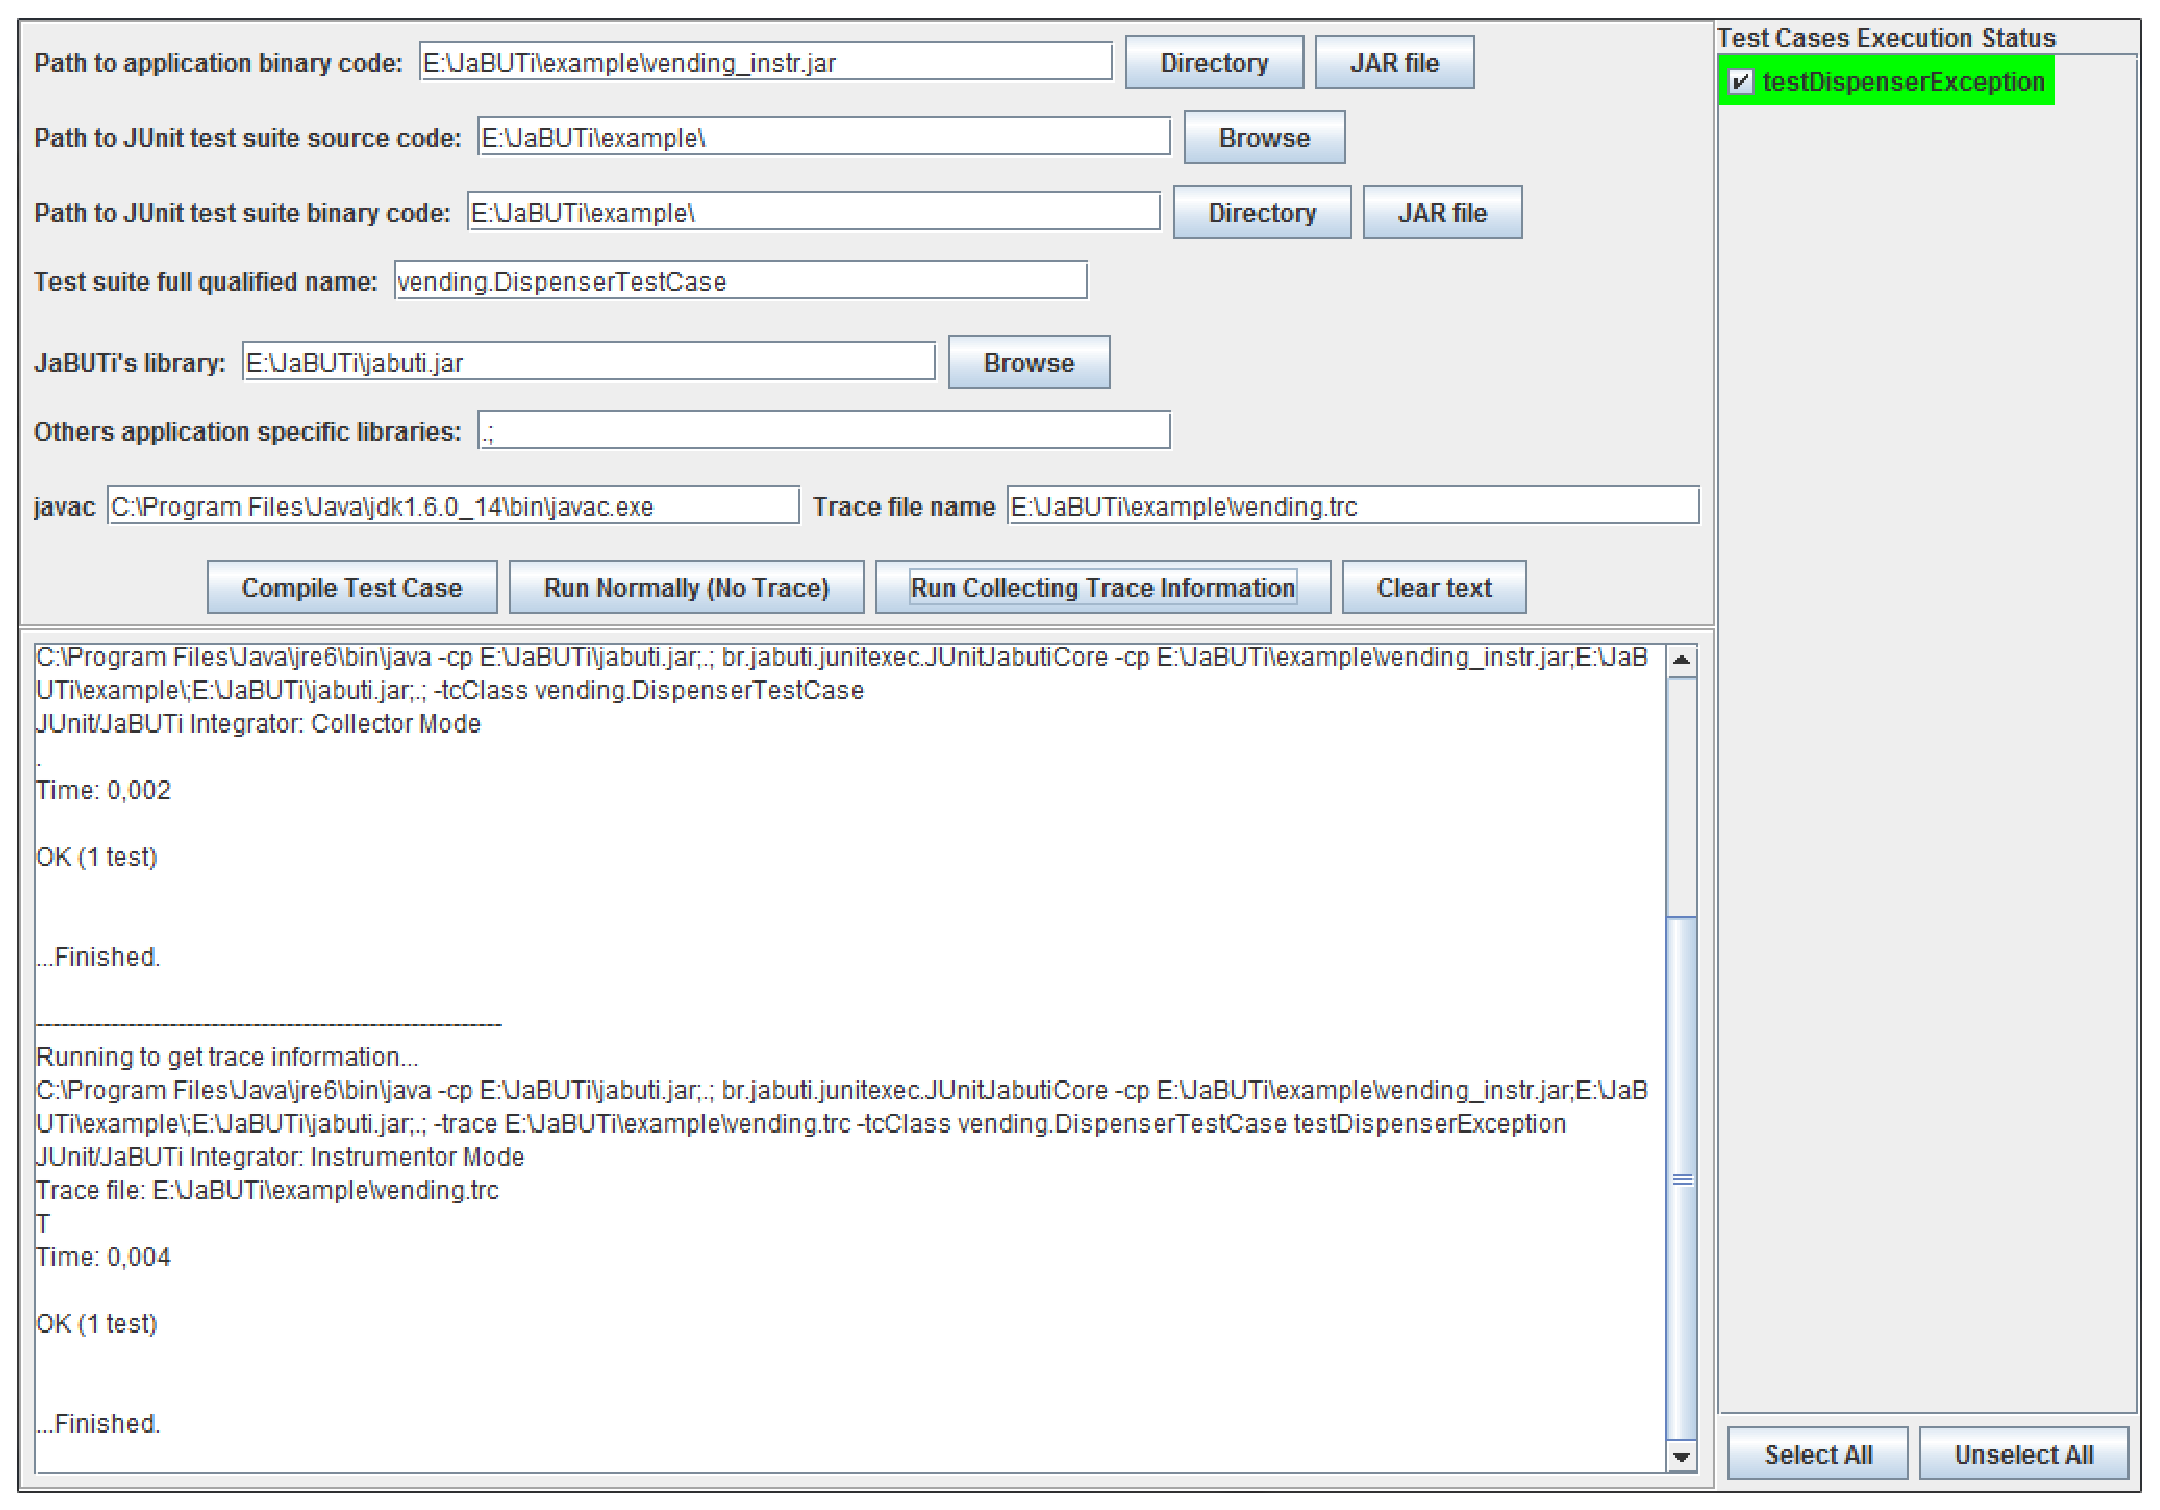
\includegraphics[width=\textwidth]{fig/importing-junit-1.eps}
%}
%\quad
%\subfigure[]{\label{fig:junit2}
\includegraphics[width=0.45\textwidth]{fig/importing-browser-1.eps}}
%
%\subfigure[]{\label{fig:junit3}
\includegraphics[width=0.45\textwidth]{fig/importing-browser-2.eps}}\quad
%\subfigure[]{\label{fig:junit4}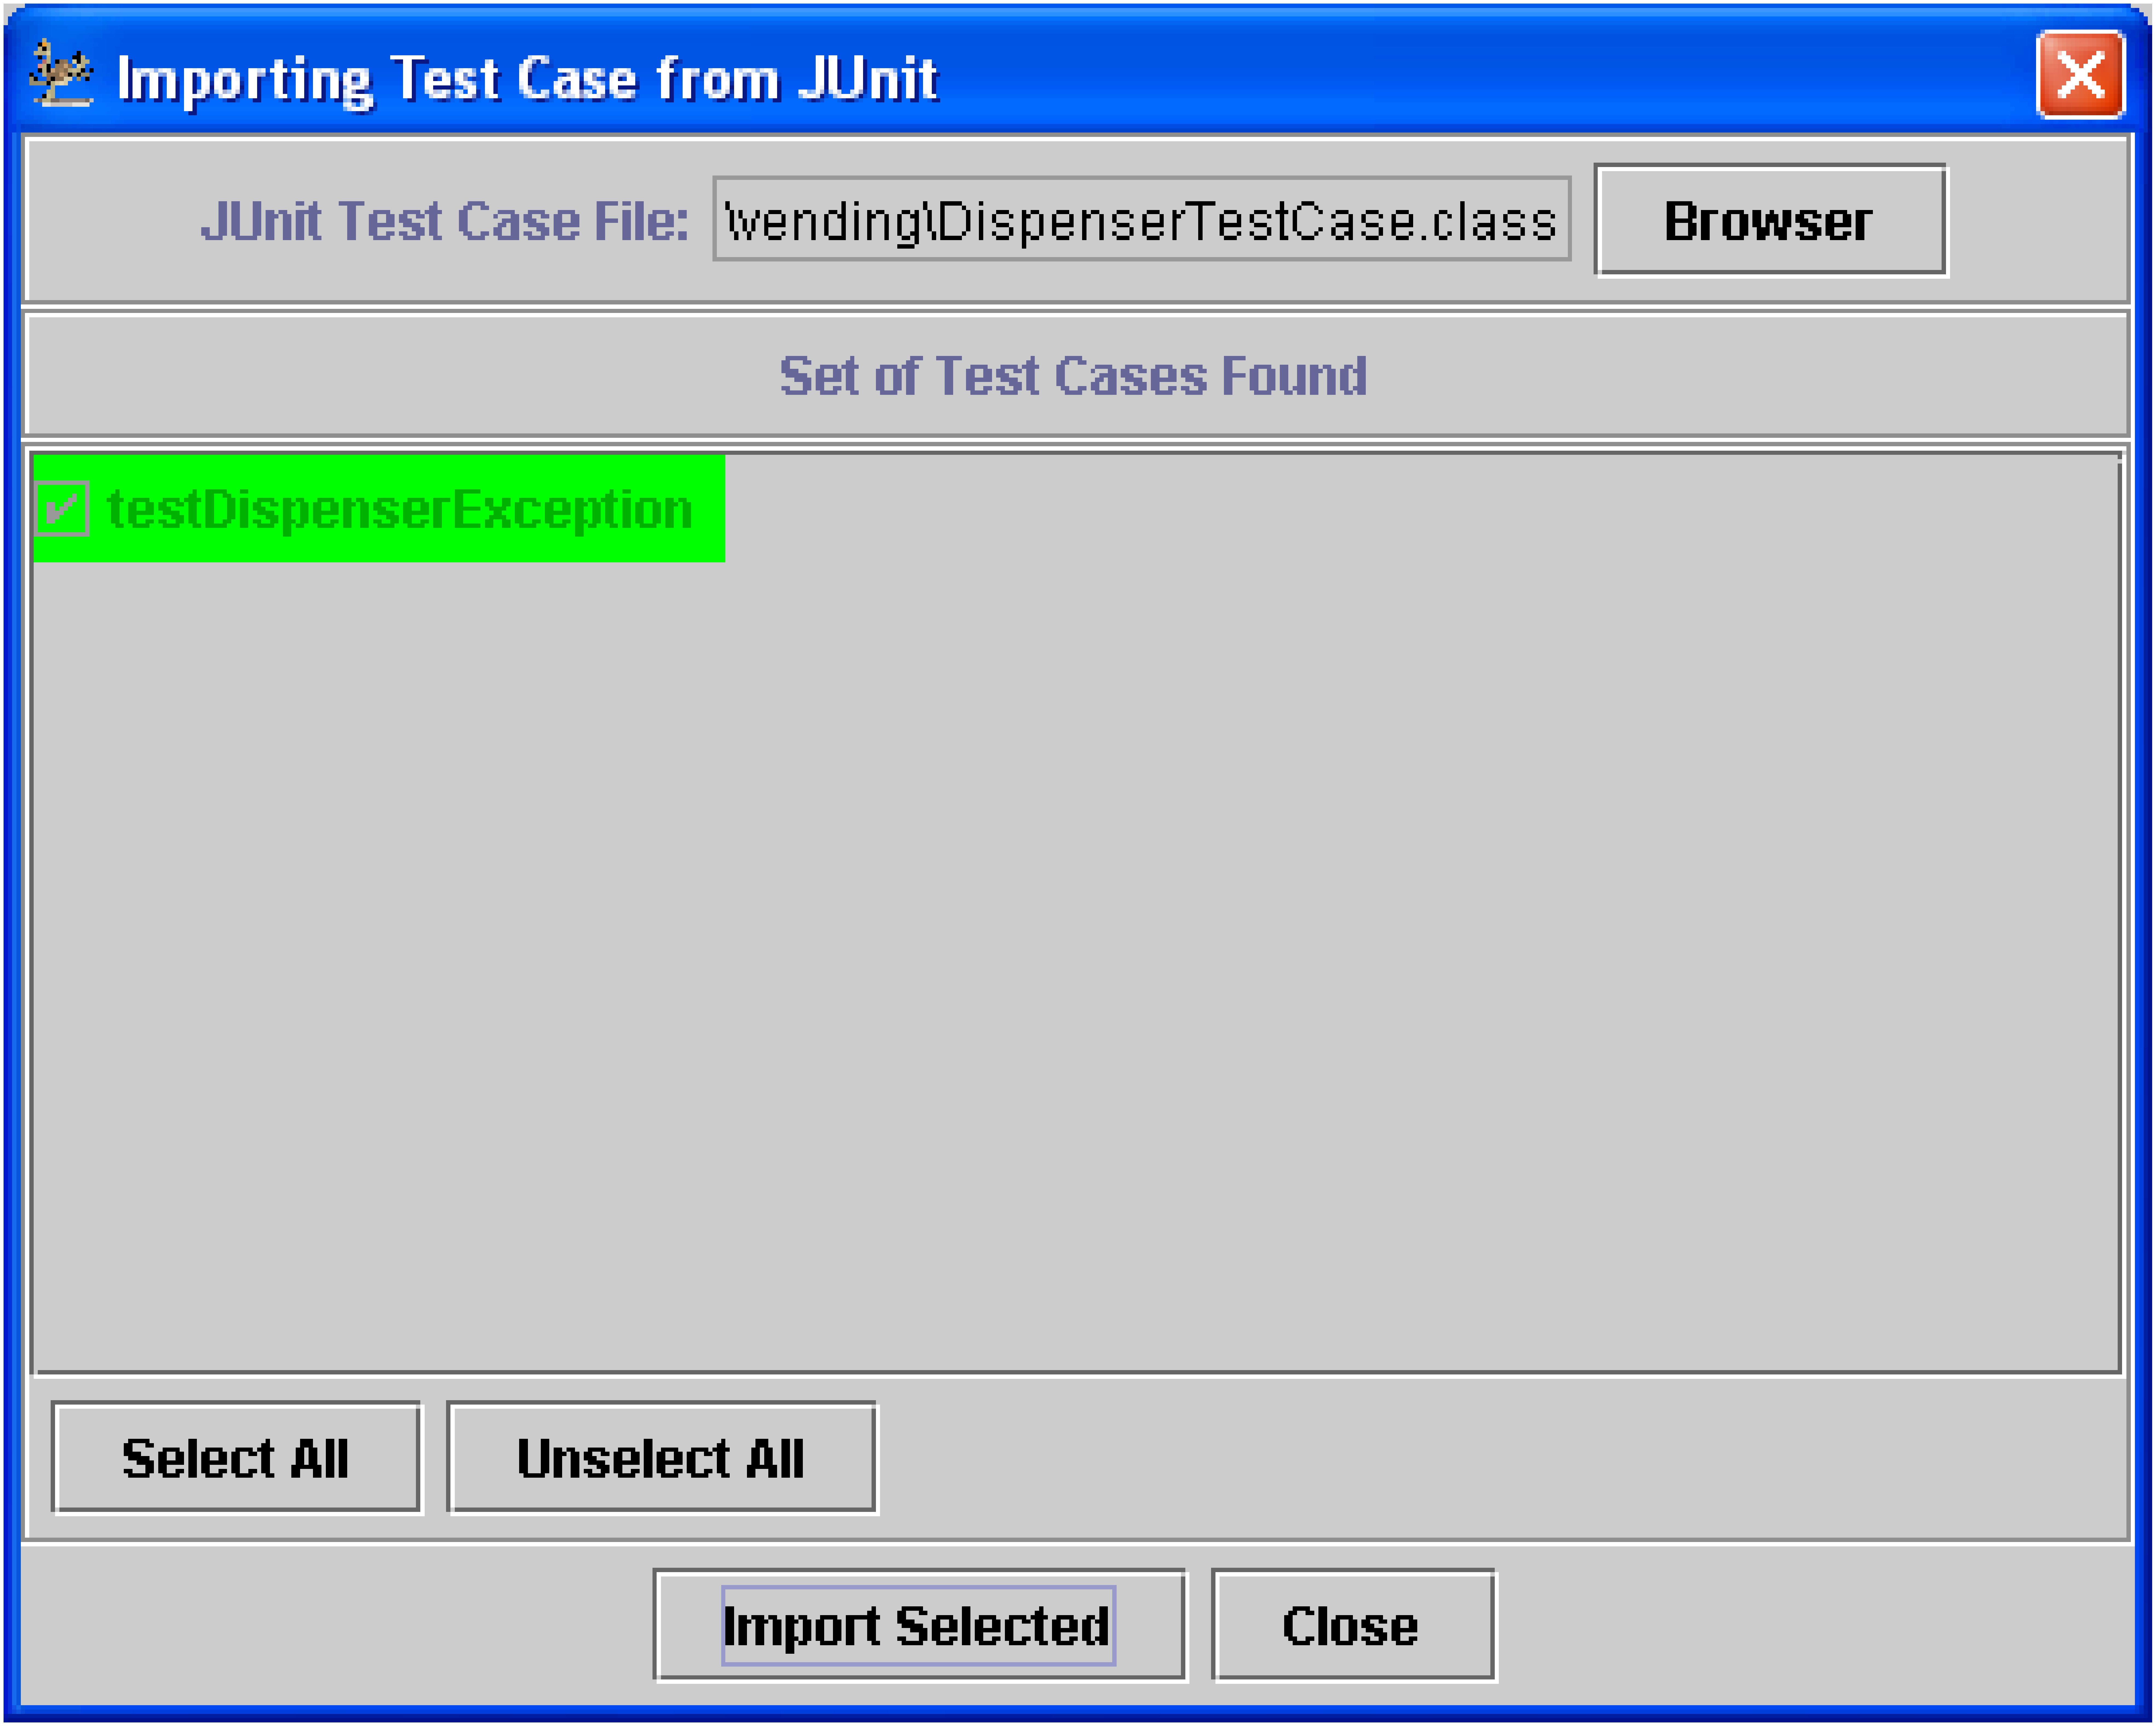
\includegraphics[width=0.45\textwidth]{fig/importing-junit-3.eps}}\quad
\caption{Importing a JUnit Test Case.}\label{fig:importing-junit}
\end{center}
\end{figure}


The fields to be entered are:

\begin{itemize}
	\item \textbf{Path to application:} automatically filled by \toolname.
	\item \textbf{Path to JUnit test suite source/binary code:} if you followed 
	the manual it should be your current path; otherwise it's the path to your
	application's source and binary codes.
	\item \textbf{Test suite full qualified name:} the full name of the JUnit test
	which will be used.
	\item \textbf{JaBUTi's library:} the .jar used to run JaBUTi.
	\item \textbf{Other application specific libraries:} other libraries your 
	application may need.
	\item \textbf{javac:} full path to your java compiler.
	\item \textbf{Trace file name:} automatically filled by \toolname.
\end{itemize}

If everything is correct, you should be able to (1) compile the test case, (2)
run it normally (to make sure it works) and (3) run it collecting trace 
information.

In our example (Figure~\ref{fig:junit1}), there is only one test
case to be imported. Observe that the name of such a test case
\pk{testDispenserException} is highlighted in green. This is
because JUnit framework provides several assertions statements,
like the one at line 22 of Figure~\ref{fig:junit}, that allows to
verify if the test case's output is according to its specification
or not. We use a green background color to represent test cases
that behave accordantly to their specifications and a red
background color to represent the ones that do not.

As soon as \toolname detects a new test case execution trace is
appended in the end of the trace file, the \pk{Update} button
becomes red indicating that the coverage needs to be updated.
Updated the coverage information,
Figure~\ref{fig:summary-method-tc6} shows the summary report by
methods and the corresponding coverage \wrt the \pk{All-Nodes-ei}
criterion. The summary report by criterion can be seen in
Figure~\ref{fig:summary-criterion-tc6}.

% This is part of the Jabuti 1.0 Manual.
% Copyright 2003 (c) Auri Marcelo Rizzo Vicenzi, Marcio Eduardo Delamaro,
% Jose Carlos Maldonado.
% See the file FDL.TXT for copying conditions.

\begin{figure}[!ht]
\begin{center}
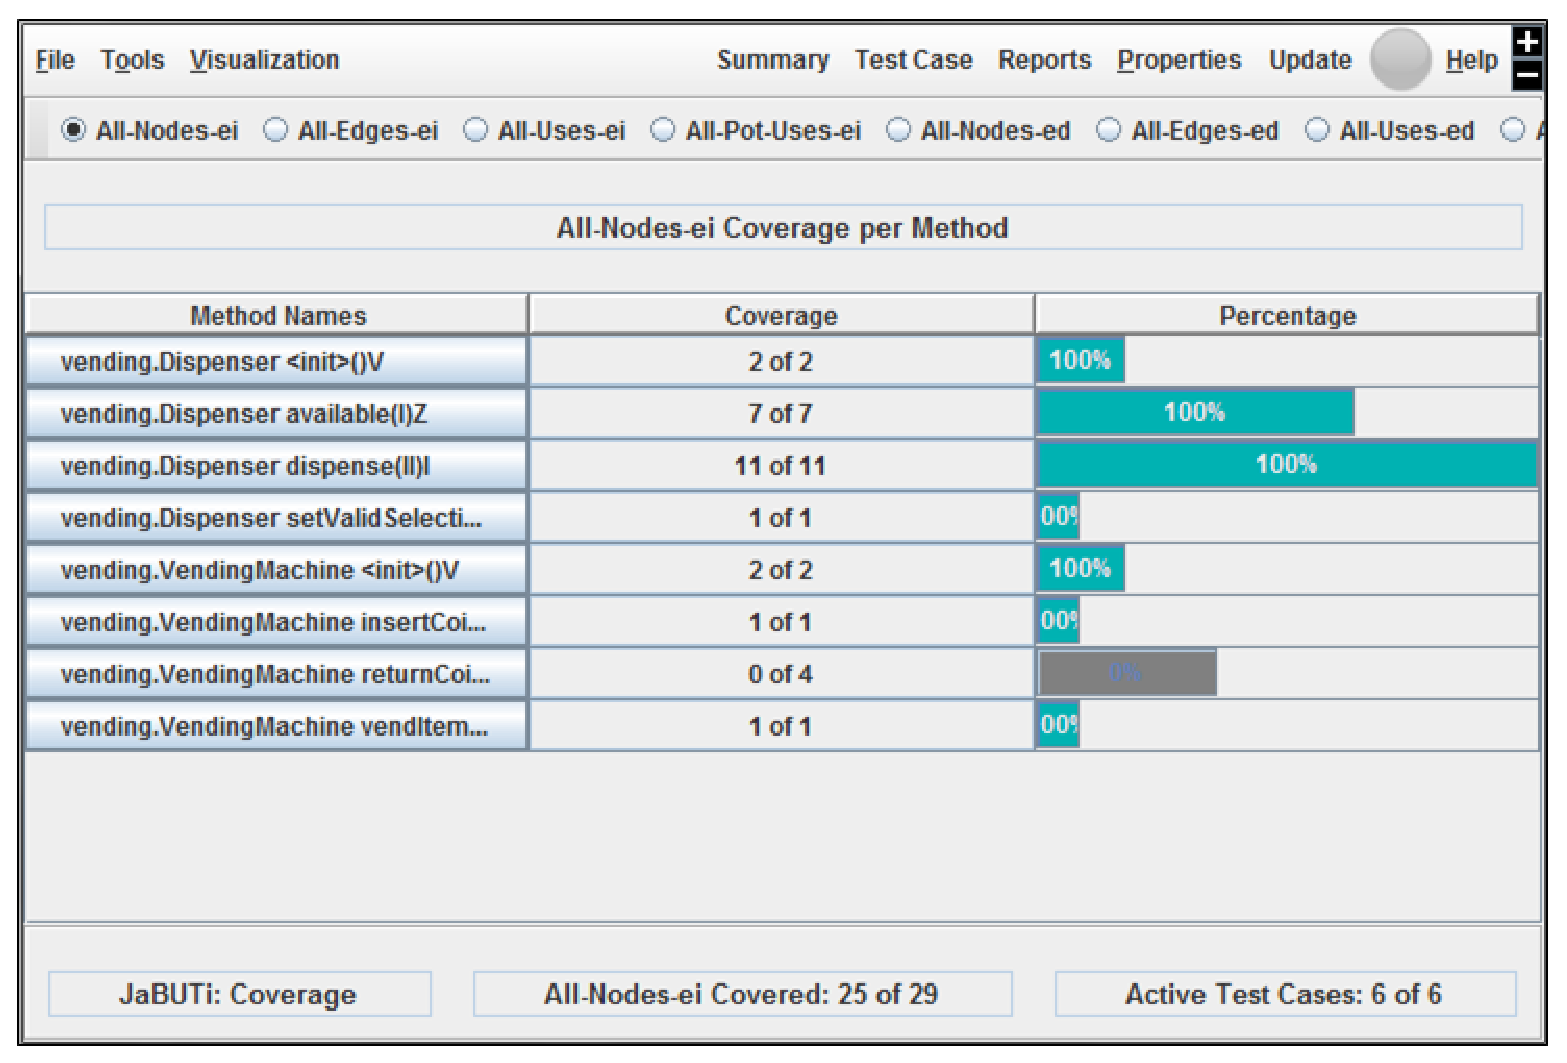
\includegraphics[width=0.70\textwidth]{fig/report-by-method-pri-nodes-tc6.eps}
\caption{\label{fig:summary-method-tc6} Updated coverage after six
test cases \wrt the \pk{All-Pri-Nodes} criterion.}
\end{center}
\end{figure}


% This is part of the Jabuti 1.0 Manual.
% Copyright 2003 (c) Auri Marcelo Rizzo Vicenzi, Marcio Eduardo Delamaro,
% Jose Carlos Maldonado.
% See the file FDL.TXT for copying conditions.

\begin{figure}[!ht]
\begin{center}
\includegraphics[width=0.70\textwidth]{fig/report-by-criterion-tc6.eps}
\caption{\label{fig:summary-criterion-tc6} Updated coverage after
six test cases \wrt all criteria.}
\end{center}
\end{figure}


After the execution of these six test cases, all methods of the
\pk{Dispenser} component are 100\% covered \wrt the
\pk{All-Nodes-ei} criterion, but this test set is adequate to the
\pk{VendingMachine} class. More specifically, the
\pk{VendingMachine.returnCoin} method is not covered yet. So,
after six test cases, the coverage of the entire project \wrt
\pk{All-Nodes-ei} and \pk{All-Nodes-ed} are 86\% and 100\%,
respectively. The coverage for the \pk{All-Edges-ei} and the
\pk{All-Edges-ed} are 82\% and 20\%, respectively, and the
coverage for the \pk{All-Uses-ei} and \pk{All-Uses-ed} are 82\%
and 0\%, respectively.

Independently of the number of test cases available, if desired,
the tester can enable/disable any combination of test cases by
accessing the \pk{Test Case $\rightarrow$ Report By Test Case}
menu option and choosing which test case should be
enabled/disabled. Once a different subset of test cases are
enabled/disabled all the coverage information should be updated by
clicking on the \pk{Update} button. Figure~\ref{fig:test-case1}
shows the complete test set with all test cases enabled.
Figure~\ref{fig:test-case2} shows the updated coverage considering
only the test cases number 2 and 5.

% This is part of the Jabuti 1.0 Manual.
% Copyright 2003 (c) Auri Marcelo Rizzo Vicenzi, Marcio Eduardo Delamaro,
% Jose Carlos Maldonado.
% See the file FDL.TXT for copying conditions.

\begin{figure}[!ht]
\begin{center}
\subfigure[]{\label{fig:test-case1}\includegraphics[width=0.45\textwidth]{fig/summary-by-test-case1.eps}}
\subfigure[]{\label{fig:test-case2}\includegraphics[width=0.45\textwidth]{fig/summary-by-test-case2.eps}}
\caption{Summary by test case: (a) all enabled, and (b) 2 and 5
enabled.}\label{fig:test-case}
\end{center}
\end{figure}


Using the resource of activate/deactivate test cases, the tester
can evaluate how the coverage changes, considering different
combinations of test case. Moreover, besides activate/deactivate
test cases, the tester can also mark a test case to be deleted.
Once a test case is marked to be deleted it is only logically
deleted. Such a test case is physically deleted when the project
is saved and closed. While the project is not closed, a test case
marked as deleted can be undeleted.

\afterpage{\clearpage}
\newpage

\subsection{How to mark a testing requirement as infeasible}

When applying structural testing criteria, one problem is to
identify infeasible testing requirements since, in general, it is
an undecidable problem. Vergilio~\cite{Vergilio97CRCA} developed
some heuristics to automatically determine infeasible testing
requirements but such heuristics are not yet implemented in
\toolname. Therefore, it is a responsibility of the tester to
identify such infeasible testing requirements.

By accessing the \pk{Visualization $\rightarrow$ Required
Elements} menu option, \toolname allows the tester to visualize
and mark testing requirements as infeasible, as well as
activate/deactivate testing requirements. Once a testing
requirement is marked as infeasible or deactivated, the
\pk{Update} button becomes red indicating that the coverage
information should be updated to reflect such a change. For
example, Figure~\ref{fig:requirements} shows part of the testing
requirements for the method \pk{Vending.returnCoin()} method,
considering the \pk{All-Nodes-ei} criterion.

% This is part of the Jabuti 1.0 Manual.
% Copyright 2003 (c) Auri Marcelo Rizzo Vicenzi, Marcio Eduardo Delamaro,
% Jose Carlos Maldonado.
% See the file FDL.TXT for copying conditions.

\begin{figure}[!ht]
\begin{center}
\includegraphics[width=0.70\textwidth]{fig/required-elements.eps}
\caption{\label{fig:requirements} \pk{Dispenser.dispense()}
required elements for the \pk{All-Pri-Nodes} criterion.}
\end{center}
\end{figure}


Considering Figure~\ref{fig:requirements}, two uncovered
requirements were marked as infeasible, primary nodes 0 and 7.
Since the tester can mark erroneously a testing requirement as
infeasible, in case such a testing requirement is covered in the
future by an additional test case, the tool indicates such a
inconsistency, highlighting the infeasible check box of a covered
testing requirement in red, as illustrated in
Figure~\ref{fig:covered-infeasible}. In this case, primary node 0
is covered by the new test case added to exercise the
\pk{Vending.returnCoin()} method, so node 0 is feasible.

During the importation of a given test case, the tester has to
check whether the obtained output is correct \wrt the
specification. As can be observed in Table~\ref{tab:adequate},
only test case number 1 does not behave according to the
specification. Once any discrepancy is detected, the fault should
be localized and corrected. One alternative for fault localization
is slicing. In the next section we describe how to use the slicing
tool implemented in \toolname to help the fault localization and
smart debugging.

% This is part of the Jabuti 1.0 Manual.
% Copyright 2003 (c) Auri Marcelo Rizzo Vicenzi, Marcio Eduardo Delamaro,
% Jose Carlos Maldonado.
% See the file FDL.TXT for copying conditions.

\begin{figure}[!ht]
\begin{center}
\includegraphics[width=0.70\textwidth]{fig/required-elements-covered-infeasible.eps}
\caption{\label{fig:covered-infeasible} \pk{Dispenser.dispense()}
infeasible requirements erroneously identified.}
\end{center}
\end{figure}


\afterpage{\clearpage}
\newpage

%------------------------------------------------------------------------------

%----------------------Slice---------------------------------------------------
% This is part of the Jabuti 1.0 Manual.
% Copyright 2003 (c) Auri Marcelo Rizzo Vicenzi, Marcio Eduardo Delamaro,
% Jose Carlos Maldonado.
% See the file FDL.TXT for copying conditions.

\section{How to use \toolname as a Slicing Tool}\label{sec:slice}

The \toolname slicing tool is available through the \pk{Tools
$\rightarrow$ Slicing Tool} menu option. The slicing tool
implements only a simple heuristic based on control-flow
information. As a future work, additional heuristics will be
implemented considering not only control-flow but also data-flow
information.

By changing to the slicing tool, the tester has to choose, among
the test cases, the ones that cause the fault and the ones that do
not reveal the fault. Based on the execution path of the failed
and succeed test cases, the tool highlights the part of the code
more probable to contain the fault.

%%%%%%%%%%%%%%%%%%%%%%%%%%%
\toolname uses a simple dynamic slice criterion, based on
control-flow information, to identify a subset of statements more
probable to contain the fault. The idea is (1) to compute the
failed set $F_S$ of \BG nodes (the execution path) of a failed
test case, which includes all statements executed by the failed
test case, (2) to compute the succeed set $S_S$ of \BG nodes
considering succeed test case(es), and (3) to calculate the
difference and the intersection of these sets to prioritize the
statements executed by the failed test case.

Using such an approach, instead of the complete set of \BG nodes
$N$ (which represents all statements of a method), the tester has
only to consider the subset of \BG nodes present in $F_S$, since
the other \BG nodes contains the statements not executed by the
failed test case and cannot contain the fault. Moreover,
considering the subset of nodes executed by the succeed test
cases, the most probably location of the fault is in the
statements executed by the failed test case but not executed by
the succeed test cases, \ie, the subset $F_S \setminus S_S$. Thus,
such a subset of statements has a highest priority and should be
analyzed first. If the fault is not located on this subset, due to
data dependence that can lead to a data-flow dependent fault, the
tester has to analyze the other statements executed by both the
failed and by the succeed test cases, \ie, the subset $F_S \cap
S_S$. In this way, we can provide an incremental search for the
fault, trying to reduce the time and the cost to locate the fault
in a program.

For example, consider the \BG presented in
Figure~\ref{fig-average-bcfg}. $N$ is the complete set of \BG
nodes ($N = \{0, 15, 34, 43, 54, 54.82, 60, 60.82, 74, 74.82, 79,
91, 97\}$). Suppose a failed test case that goes though \BG nodes
$F_S = \{0, 34, 15, 34, 43, 54, 54.82, 91, 97\}$ and a successful
test case that goes trough \BG nodes $S_S = \{0, 34, 43, 60,
60.82, 91, 97\}$. The most probably locations for the fault are in
the statements in nodes 15, 54 or 54.82, since they are only
executed by the failure test case ($F_S \setminus S_S$). If the
fault is not located on such statements, it will be found in the
other statements that compose the \BG nodes 0, 34, 43, 91 and 97
($F_S \cap S_S$). All the other \BG nodes have not to be analyzed.

The approach described above is based only on control-flow
information. The success of such an approach depends on which test
cases are selected as the successful test cases. It is important
to select successful test cases that execute the related
functionalities of the program as the ones executed by the failure
test case. In this way, the difference between the two sets $F_S$
and $S_S$ will result in subset with a few \BG nodes, reducing the
number of statements that have to be analyzed first.

In our Vending Machine example, test case \pk{0001} reveals the
fault and test case \pk{0006} does not. The tester can first
select only the failed test case, as illustrated in
Figure~\ref{fig:slice-test-case1}, and checks the execution path
of this test case as illustrated in
Figure~\ref{fig:slice-source-fail}. The red lines indicate the
statements that are executed by the failed test case and the white
lines indicates the statements not executed. Since there is a
fault, it must be located among these red statements.

% This is part of the Jabuti 1.0 Manual.
% Copyright 2003 (c) Auri Marcelo Rizzo Vicenzi, Marcio Eduardo Delamaro,
% Jose Carlos Maldonado.
% See the file FDL.TXT for copying conditions.

\begin{figure}[!ht]
\begin{center}
\subfigure[]{\label{fig:slice-test-case1}\includegraphics[width=0.45\textwidth]{fig/slicing-fail-test-case.eps}}
\subfigure[]{\label{fig:slice-test-case6}\includegraphics[width=0.45\textwidth]{fig/slicing-fail-1success-test-case.eps}}
\caption{Slicing tool test case selection: (a) only the failed
test case, and (b) a failed and a succeed test
cases.}\label{fig:slice-test-cases}
\end{center}
\end{figure}


After having observed the failed test case execution path, the
tester can enable one or more additional succeed test cases
(Figure~\ref{fig:slice-test-case6}), such that the tool can
identify, among the statements executed ny the failed test case,
the dice more probable to contain the fault (statements only
executed by the failed test case) and the ones less probable (the
ones executed for both the failed and the succeed test cases.)
Figure~\ref{fig:slice-source-fail-success} shows in yellow
(weight~1) the statements touched by test cases number \pk{0001}
and \pk{0006} and in red (weight~2) the statements only executed
by test case number~\pk{0001}.

The rationale of such an approach is that, in theory, the fault is
more probable to be located at the statements executed only by the
failed test case. Although, it can happen that the fault is
localized in other than the red statements, but the red points can
be used at least as a good starting point, trying to reduce the
search space for fault localization.

Once the fault is located and corrected, the testing activity is
restarted by creating a new project to revalidate the corrected
program. In this case, previous test sets can be used to
revalidate the behavior of the new program and also to check if
new faults were not introduced by the changes.

% This is part of the Jabuti 1.0 Manual.
% Copyright 2003 (c) Auri Marcelo Rizzo Vicenzi, Marcio Eduardo Delamaro,
% Jose Carlos Maldonado.
% See the file FDL.TXT for copying conditions.

\begin{figure}[!ht]
\begin{center}
\subfigure[]{\label{fig:slice-source-fail}\includegraphics[width=0.45\textwidth]{fig/slicing-source-fail.eps}}
\subfigure[]{\label{fig:slice-source-fail-success}\includegraphics[width=0.45\textwidth]{fig/slicing-source-fail-1success.eps}}
\caption{Highlighted execution path: (a) fail test case execution
path, and (b) fail test case execution path intersected by the
success test case execution path.}\label{fig:slice-source}
\end{center}
\end{figure}


%------------------------------------------------------------------------------

%----------------------Slice---------------------------------------------------
% This is part of the Jabuti 1.0 Manual.
% Copyright 2003 (c) Auri Marcelo Rizzo Vicenzi, Marcio Eduardo Delamaro,
% Jose Carlos Maldonado.
% See the file FDL.TXT for copying conditions.

\section{How to use the \toolname's Static Metrics Tool}\label{sec:metrics}

Adicionalmente, na Se��o~\ref{metricas:outras}, a m�trica que
avalia a complexidade ciclom�tica de McCabe~\cite{Pressman00SEPA}
de cada m�todo tamb�m foi implementada para identificar os m�todos
de ``maior'' complexidade dentro de uma dada classe.

\subsection{LK's Metrics Applied to Classes}\label{metricas:lk}

\subsubsection{NPIM -- Number of public instance methods in a class}

M�trica calculada atrav�s da contagem do n�mero de m�todos de
inst�ncia p�blicas na classe.

\subsubsection{NIV -- Number of instance variables in a class}

M�trica calculada atrav�s da contagem do n�mero de vari�veis de
inst�ncia na classe, o que inclui as vari�veis \textit{public},
\textit{private} e \textit{protected} dispon�veis para as
inst�ncias.

\subsubsection{NCM -- Number of class methods in a class}

M�trica calculada atrav�s da contagem do n�mero de m�todos
\textit{static} na classe.

\subsubsection{NCV -- Number of class variables in a class}

M�trica calculada atrav�s da contagem do n�mero de vari�veis
\textit{static} na classe.

\subsubsection{ANPM -- Average number of parameters per method}

M�trica calculada atrav�s da divis�o entre o somat�rio do n�mero
de par�metros de cada m�todo da classe pelo n�mero total de
m�todos da classe.

Varia��o: n�mero m�ximo de par�metros em um m�todo da classe.

\subsubsection{AMZ -- Average method size}

M�trica calculada atrav�s da divis�o entre a soma do n�mero de
linhas de c�digo dos m�todos da classe pelo n�mero de m�todos na
classe (soma dos m�todos inst�ncia e classe).

Varia��es: m�dia do n�mero de instru��es do bytecode e tamanho do
bytecode.

\subsubsection{UMI -- Use of multiple inheritance}

Como a heran�a m�ltipla n�o se aplica � linguagem JAVA ser�
definida uma varia��o � esta m�trica.

Varia��o: n�mero de interfaces implementadas pela classe
(\textit{Number of interfaces implemented} - NINI).

\subsubsection{NMOS -- Number of methods overridden by a subclass}

M�trica calculada atrav�s da contagem do n�mero de m�todos
definidos na subclasse com o mesmo nome de m�todos de sua
superclasse.

\subsubsection{NMIS -- Number of methods inherited by a subclass}

M�trica calculada atrav�s da contagem do n�mero de m�todos
herdados pela subclasse de suas superclasses.


\subsubsection{NMAS -- Number of methods added by a subclass}

M�trica calculada atrav�s da contagem do n�mero de novos m�todos
adicionados pelas subclasses.

\subsubsection{SI -- Specialization index}

M�trica calculada atrav�s da divis�o entre o resultado da
multiplica��o de NMOS e DIT (m�trica de CK) pelo n�mero total de
m�todos.


\subsection{CK's Metrics Applied to Classes}\label{metricas:ck}

\subsubsection{NOC -- Number of Children}

M�trica calculada atrav�s da contagem do n�mero de subclasses
imediatas subordinadas � classe na �rvore de hierarquia.

\subsubsection{DIT -- Depth of Inheritance Tree}

� o maior caminho da classe � raiz na �rvore de hierarquia de
heran�a. Interfaces tamb�m s�o consideradas, ou seja, o caminho
atrav�s de uma hierarquia de interfaces tamb�m pode ser o que d� a
profundidade de uma classe.

Varia��o: como a representa��o de programa utilizada n�o inclui
todas as classes at� a raiz da �rvore de hierarquia, ser�
utilizado o caminho da classe at� a primeira classe que n�o
pertence � estrutura do programa.


\subsubsection{WMC -- Weighted Methods per Class}

 M�trica calculada atrav�s da soma da complexidade de cada m�todo.
 N�o se define qual tipo de complexidade pode ser utilizada, assim
 ser�o aplicadas as seguintes varia��es:

 \begin{itemize}
 \item Utiliza-se o valor 1 como complexidade de cada m�todo;
 assim WMC\_1 � o numero de m�todos na classe;
 \item Utiliza-se a m�trica CC para a complexidade de cada m�todo;
 esta m�trica ser� chamada WMC\_CC;
 \item Utiliza-se a m�trica LOCM para a complexidade de cada m�todo;
 esta m�trica ser� chamada WMC\_LOCM;
 \item Utiliza-se o tamanho do m�todo (n�mero de instru��es)
 para a complexidade de cada m�todo;
 esta m�trica ser� chamada WMC\_SIZE;
 \end{itemize}

\subsubsection{LCOM -- Lack of Cohesion in Methods}

M�trica calculada atrav�s da contagem do n�mero de pares de
m�todos na classe que n�o compartilham vari�veis de inst�ncia
menos o n�mero de pares de m�todos que compartilham vari�veis de
inst�ncia. Quando o resultado � negativo, a m�trica recebe o valor
zero. Os m�todos est�ticos n�o s�o considerados na contagem, uma
vez que s� as vari�veis de inst�ncia s�o tomadas.

Varia��es:
\begin{itemize}
\item Considerar s� a coes�o entre m�todos est�ticos; esta m�trica
ser� chamada LCOM\_2; \item Considerar a coes�o de m�todos
est�ticos ou de inst�ncia; esta m�trica, chamada LCOM\_3 pode ser
calculada como $LCOM\_ - LCOM\_2$;
\end{itemize}

\subsubsection{RFC -- Response for a Class}

M�trica calculada atrav�s da soma do n�mero de m�todos da classe
mais os m�todos que s�o invocados diretamente por eles. � o n�mero
de m�todos que podem ser potencialmente executados em resposta a
uma mensagem recebida por um objeto de uma classe ou por algum
m�todo da classe. Quando um m�todo polim�rfico � chamado para
diferentes classes, cada diferente chamada � contada uma vez.

\subsubsection{CBO -- Coupling Between Object}

H� acoplamento entre duas classes quando uma classe usa m�todos
e/ou vari�veis de inst�ncia de outra classe. M�trica calculada
atrav�s da contagem do n�mero de classes �s quais uma classe est�
acoplada de alguma forma, o que exclui o acoplamento baseado em
heran�a. Assim, o valor CBO de uma classe A � o n�mero de classes
das quais a classe A utiliza algum m�todo e/ou vari�vel de
inst�ncia.


\subsection{Another Metrics Applied to Methods}\label{metricas:outras}


\subsubsection{CC -- Cyclomatic Complexity Metric}

M�trica que calcula a complexidade do m�todo, atrav�s dos grafos
de fluxo de controle que descreve a estrutura l�gica do m�todo.

Os grafos de fluxo consistem de n�s e ramos, onde os n�s
representam comandos ou express�es e os ramos representam a
transfer�ncia de controle entre estes n�s.

A m�trica pode ser calculada das seguintes formas:

\begin{itemize}

\item O n�mero de regi�es do grafo de fluxo corresponde �
Complexidade Ciclom�tica;

\item A Complexidade Ciclom�tica, V(G), para o grafo de fluxo G �
definida como:

\begin{center}

V(G) = E - N + 2

\end{center}

onde, V(G) mede os caminhos linearmente independentes encontrados
no grafo, E � o n�mero de ramos do grafo de fluxo e N o n�mero de
n�s.

\item A Complexidade Ciclom�tica, V(G), para o grafo de fluxo G �
definida como:

\begin{center}

V(G) = P(G)+1

\end{center}

onde, P(G) � o n�mero de n�s predicativos contidos no grafo de
fluxo G. Os n�s predicativos s�o comandos condicionais
(\textit{if}, \textit{while}, ...) com um ou mais operadores
booleanos (\textit{or}, \textit{and}, \textit{nand},
\textit{nor}). Um n� � criado para cada n� `a' ou `b' de um
comando \verb+IF a OR b+.

\end{itemize}

Outras formas de se calcular a Complexidade Ciclom�tica s�o:

\begin{itemize}

\item V(G) = n�mero de regi�es de G;

\item V(G) = n�mero de ramos - n�mero de n�s + 2;

\item V(G) = n�mero de n�s predicativos + 1.

\end{itemize}

Varia��es: a m�trica � aplicada a m�todos mas pode ser aplica �
classe atrav�s da soma ( ver WMC\_CC), da m�dia (que ser� chamada
CC\_AVG) e do m�ximo (CC\_MAX) entre os m�todos.

\subsection{The Static Metrics GUI}

The set of static metrics implemented in \toolname can be accessed
by the \pk{Visualization $\rightarrow$ Complexity Metrics} menu
option. Figure~\ref{fig:class-metrics} illustrates the window that
will be displayed, considering the \pk{vending\prjext} project
file. Each line corresponds to a given user class and each column
is the resultant value of a given static metric applied to such a
class. Observe that not only the classes under testing are
displayed but also the other user classes required by the base
class. A user class not required to be instrumented appears
between braces. The idea is to allow the tester to visualize the
metrics with respect to all possible classes that can be
instrumented such that he/she can decide later to select such
classes to be tested.

By moving the mouser cursor onto the head of a given column, it is
displayed a tip, giving a brief description of the corresponding
metric of such a column. For example,
Figure~\ref{fig:class-metrics-tip} shows the tip for the \pk{CBO}
metrics, responsible to measure the coupling between objects.

% This is part of the Jabuti 1.0 Manual.
% Copyright 2003 (c) Auri Marcelo Rizzo Vicenzi, Marcio Eduardo Delamaro,
% Jose Carlos Maldonado.
% See the file FDL.TXT for copying conditions.

\begin{figure}[!ht]
\begin{center}
\subfigure[Metrics
view]{\label{fig:class-metrics}\includegraphics[width=0.7\textwidth]{fig/metrics-view-edited.eps}}

\subfigure[Metrics tool
tip]{\label{fig:class-metrics-tip}\includegraphics[width=0.7\textwidth]{fig/metrics-tool-tip.eps}}
\caption{Static Metrics Tool's graphical
interface.}\label{fig:metrics-gui}
\end{center}
\end{figure}


%------------------------------------------------------------------------------

\afterpage{\clearpage}
\newpage

%----------------------  Mobile devices ----------------------------------------
%% This is part of the Jabuti 1.0 Manual.
% Copyright 2003 (c) Auri Marcelo Rizzo Vicenzi, Marcio Eduardo Delamaro,
% Jose Carlos Maldonado.
% See the file FDL.TXT for copying conditions.

\section{\toolname em dispositivos m�veis}
A ferramenta \toolname foi adaptada para ser utilizada
no teste de programas Java que rodam em dispositivos
m�veis como PDAs ou telefones celulares. Mais precisamente,
que est�o de acordo com o perfil MIDP (Mobile Information
Device Profile).

Essa se��o descreve as diferen�as na utiliza��o da ferramenta para
o teste desse tipo de software. As mudan�as de procedimento dizem
respeito, principalmente, � instrumenta��o e execu��o dos casos de
teste. Como os programas instrumentados devem executar em
dispositivos m�veis,\footnote{Quando nos referimos a dispositivos m�veis
inclu�mos os simuladores que, apesar de executarem no desktop, est�o
sujeitos aos mesmos tipos de limita��es do perfil MIDP.} o tipo de
instrumenta��o deve ser adequada �quele ambiente. Al�m disso, os
dados de execu��o (trace) devem ser analisados pela \toolname, no
desktop.

Assim, a primeira mudan�a a ser feita � a instala��o de um
servidor que vai ser respons�vel pela aquisi��o dos dados de
execu��o dos programas e a gera��o do arquivo de trace que �
tratado pela \toolname. O servidor pode ser instalado atrav�s de
um programa chamado diretamente na linha de comando ou de dentro
da pr�pria ferramenta.

Na chamada direta, o programa deve receber dois argumentos, como
mostra a descri��o abaixo:
\begin{verbatim}
> java -cp <classpath Jabuti> br.jabuti.device.ProberServer <port> <filename>
\end{verbatim}

O primeiro argumento indica o n�mero da porta � qual o servidor
vai se anexar. O segundo � o nome de um arquivo de configura��o
que descreve quais s�o os programas que devem ser tratados pelo
servidor. Um servidor pode tratar de mais de um programa em
execu��o ao mesmo tempo. O formato do arquivo de configura��o �
bastante simples. Ele possui, para cada programa a ser tratado,
duas linhas, contendo a identifica��o do programa e o nome do
arquivo de trace onde os dados de execu��o devem ser gravados.
Por exemplo:

\begin{verbatim}
PropExample
/home/user/Demos/PropExample.trc
Foo
/home/foo/foo.trc
\end{verbatim}

No arquivo de configura��o acima, dois programas poder�o ser
tratados pelo servidor. Um batizado de ```PropExample'' e outro
batizado de ``Foo''. Quando o servidor recebe dados de execu��o do
primeiro, esses dados ser�o gravados no arquivo
``/home/user/Demos/PropExample.trc'' e do segundo, no arquivo
``/home/foo/foo.trc''. Note que o nome do programa n�o est�
relacionado com a sess�o de teste criada para o teste. Esse nome �
atribu�do pelo testador no momento da instrumenta��o, como ser�
descrito adiante.

Um exemplo de utiliza��o do comando que instala o servidor seria:

\begin{verbatim}
java -cp Jabuti-bin.zip br.jabuti.device.ProberServer 1988 config.txt
\end{verbatim}

A instala��o atrav�s da ferramenta \toolname � feita atrav�s da
op��o ``Properties/Test Server''. Com essa opera��o abre-se a
janela mostrada na Figura~\ref{fig:testserver}. Nela o testador
deve selecionar a porta em que o servidor ser� instalado e o
arquivo de configura��o. Pode, tamb�m, editar esse arquivo e
salv�-lo, se necess�rio. O testador deve, ainda, selecionar a op��o
``Mobile device'', que indica o tipo de servidor desejado.

\begin{figure}[!ht]
\begin{center}
\includegraphics[width=0.50\textwidth]{fig/testserver.eps}
\caption{\label{fig:testserver}Instala��o do servidor para dispositivos
m�veis.}
\end{center}
\end{figure}

Outra diferen�a na execu��o da sess�o de teste para dispositivos
m�veis est� na instrumenta��o e do programa em teste e na execu��o
dos casos de teste. O programa � instrumentado e gera-se um
arquivo .jar contendo todas as classes que comp�em o programa,
instrumentando-se aquelas que foram escolhidas na cria��o do
projeto de teste. O comando que realiza a instrumenta��o � o
seguinte:

\begin{verbatim}
java -cp <classpath Jabuti> br.jabuti.device.ProberInstrum <op��es> <classe base>
\end{verbatim}

A classe base refere-se ao nome da classe do MIDlet que se deseja
testar. Deve-se notar que num �nico ``pacote'' � poss�vel
colocar-se diversos MIDlets distintos. Por�m, somente um pode ser
instrumentado de cada vez. As op��es de instrumenta��o s�o as
seguintes:

\begin{description}
\item [<-d diret�rio>:] indica o diret�rio no qual se encontra o
arquivo de projeto. � opcional e, se n�o for fornecido, assume-se
o diret�rio corrente;
\item[<-p projeto>:] nome do arquivo de projeto, criado pela
\toolname, que corresponde � sess�o de teste. Argumento
obrigat�rio;
\item[<-o arquivo>:] d� o nome do arquivo .jar onde ser�o
gravadas as classes instrumentadas do programa. Como as classes
instrumentadas fazem chamadas a m�todos localizados em classes da
\toolname, essas classes s�o, tamb�m, adicionadas ao arquivo de
sa�da;
\item [<-name midlet id>:] � o nome que ser� dado ao programa em
teste. � esse nome que identifica o MIDlet para o servidor de
teste, como visto anteriormente;
\item [<-h end. servidor>:] esse par�metro fornece o endere�o
onde o servidor de teste foi instalado, no formato
``128.123.82.71:1988'' ou ``myserver.com.br:1988''. � um par�metro
opcional. Caso n�o seja fornecido, os dados n�o ser�o enviados a
nenhum servidor. N�o utilizar essa op��o torna a execu��o do
programa in�til em termos de teste, propriamente dito, mas pode
ser �til para a depura��o da ferramenta. Os dados de teste podem
ser exibidos na sa�da padr�o ou num arquivo, como ser� visto a
seguir;
\item [<-temp arquivo>:] utiliza o arquivo especificado como
dep�sito tempor�rio dos dados de trace, no dispositivo. Isso
permite que, em dispositivos que possuem sistema de arquivos, os
dados fiquem armazenados ali, salvando espa�o na mem�ria
principal. O nome ``\_\_STDOUT\_\_'' indica que os dados devem ser
escritos na sa�da padr�o do didpositivo m�vel. Isso s� faz sentido se a
execu��o for feita num simulador no desktop, poi, em geral os
dispositivos m�veis n�o apresentam resultados na sa�da padr�o;
\item [<-mem valor>:] especifica um threshold de mem�ria
dispon�vel que deve ser respeitado para armazenamento dos dados de
trace. Quando a quantidade de mem�ria cai abaixo desse valor os
dados s�o enviados para o servidor de teste, ou armazenados no
arquivo tempor�rio. O valor pode ser dado em bytes (por exemplo,
1024), em kbytes ou em mbytes (por exemplo, 128K ou 3M). � um
par�metro opcional e, se n�o fornecido, assume o valor zero,
indicando que n�o existe threshold e os dados s�o sempre
armazenados, at� que a execu��o termine;
\item [<-nokeepalive>:] se utilizado, esse par�metro indica que a
conex�o (TCP) entre o dispositivo e o servidor de teste n�o deve
ser mantida durante toda a execu��o do programa. Assim, cada vez
que dados devem ser transmitidos, uma nova conex�o � criada. Isso
pode representar economia nos dispositivos em que a utiliza��o de
rede � cara e paga em fun��o do tempo de utiliza��o. A utiliza��o
da op��o ``<-temp arquivo>'' j� determina que a conex�o n�o
ser� mantida viva pois todos os dados de execu��o s�o gravados no
arquivo tempor�rio e somente no final da execu��o do MIDlet os
dados s�o enviados ao servidor.
\end{description}

Seguem-se alguns exemplos da utiliza��o do instrumentador, com
alguma combina��es de par�metros. \\

\hrule
\begin{verbatim}
java -cp Jabuti-bin.zip br.jabuti.device.ProberInstrum -name PropExample
-p Propexample.jbt -o PropExample.jar -h 200.188.151.130:2000 example.PropExample
\end{verbatim}

Nesse exemplo, o programa, cuja sess�o de teste est� descrita no
projeto chamado ``PropExample'', recebeu o nome de
``PropExample'', que tamb�m � o nome dado ao arquivo .jar de
sa�da. Os dados de trace ser�o enviados ao endere�o
``200.188.151.130:2000'' e a classe do MIDlet �
``example.PropExample''. Como n�o foi estabelecido um threshold
de mem�ria, todos os dados ser�o armazenados e somente enviados no
final da execu��o do programa. Mesmo assim, a conex�o entre o
dispositivo e o servidor de teste � aberta no in�cio da execu��o
do MIDlet e permanece aberta at� o final do envio dos dados. \\

\hrule
\begin{verbatim}
java -cp Jabuti-bin.zip br.jabuti.device.ProberInstrum -name PropExample
-p Propexample.jbt -o PropExample.jar -h 200.188.151.130:2000 -nokeepalive
example.PropExample
\end{verbatim}

O mesmo do exemplo anterior, por�m a conex�o n�o permanece aberta
o tempo todo. Ela s� � criada no in�cio da execu��o, para que seja verificada
se realmente pode ser criada e depois, no final, quando os dados
forem enviados. \\

\hrule
\begin{verbatim}
java -cp Jabuti-bin.zip br.jabuti.device.ProberInstrum -name PropExample
-p Propexample.jbt -o PropExample.jar -h 200.188.151.130:2000 -nokeepalive
-mem 512M example.PropExample
\end{verbatim}

Nesse caso, os dados s�o enviados periodicamente, quando a
quantidade de mem�ria dispon�vel estiver abaixo do valor
estabelecido, ou seja 512 mega-bytes. Como � improv�vel que algum
dispositivo tenha uma mem�ria livre desse tamanho, o que deve
ocorrer � que a cada dado de trace coletado, este seja
imediatamente enviado para o servidor. Como a op��o
``-nokeepalive'' foi utilizada, isso significa que a cada dado
coletado, uma nova conex�o � criada, o que pode interferir
sobremaneira na execu��o do MIDlet. \\

\hrule
\begin{verbatim}
java -cp Jabuti-bin.zip br.jabuti.device.ProberInstrum -name PropExample
-p Propexample.jbt -o PropExample.jar -h 200.188.151.130:2000 -nokeepalive
-temp /root1/temp.txt example.PropExample
\end{verbatim}

Com a utiliza��o do arquivo tempor�rio, os dados de trace s�o
sempre enviados para esse arquivo e somente no final enviados para
o servidor. Assim n�o s�o criadas, constantemente, conex�es.\\

\hrule
\begin{verbatim}
java -cp Jabuti-bin.zip br.jabuti.device.ProberInstrum -name PropExample
-p Propexample.jbt -o PropExample.jar -temp __STDOUT__ example.PropExample
\end{verbatim}

Os dados de teste coletados s�o apresentados na sa�da padr�o do
dispositivo. Como n�o foi fornecido o threshold de mem�ria esse
resultado s� � apresentado no final da execu��o. \\

\hrule
\ \\

Depois de instrumentadas as classes, � necess�rio ainda mais um
passo para que o programa possa ser executado. � a pr�-verifica��o
do bytecode e o empacotamento num �nico arquivo. Isso � feito com
o comando descrito a seguir:

\begin{verbatim}
> java -cp <classpath Jabuti> br.jabuti.device.Preverify <op��es>
\end{verbatim}

Os argumentos fornecidos para a execu��o s�o os seguintes:

\begin{description}
\item [<-source arquivo>:] esse argumento � obrigat�rio e indica
qual � o arquivo .jar onde est�o as classes originais do programa
a ser carregado no dispositivo m�vel. Note-se que, como comentado
anteriormente, esse arquivo pode conter diversos MIDlets, al�m
daquele sendo testado;
\item [<-instr arquivo">:] � o nome do arquivo .jar que foi criado
no passo anterior, a instrumenta��o. O que o programa ir� fazer �
substituir no arquivo original, as classes que foram
instrumentadas, mantendo as demais como est�o;
\item[<-o arquivo>:] indica o nome do arquivo .jar de sa�da. � um
argumento opcional e, caso n�o seja fornecido, assume-se o mesmo
nome do arquivo original. Nesse caso, o arquivo original �
sobrescrito;
\item [<-jad arquivo>:] especifica o nome do arquivo .jad
a ser gerado, com as informa��es sobre o ``pacote'' gerado. �
opcional e, se n�o for fornecido, nada � gerado;
\item [<-WTK diret�rio>:] a \toolname n�o realiza a pr�-verifica��o
por si s�. Ela utiliza o toolkit de desenvolvimeto wireless da SUN
para efetuar tal tarefa. Por isso, o testador deve indicar qual �
o diret�rio onde encontra-se o WTK.
\end{description}

Um exemplo de sua utiliza��o seria:

\begin{verbatim}
java -cp Jabuti-bin.zip br.jabuti.device.Preverify -source Demos.jar
-instr PropExample.jar -o Demos.jar -jad Demos.jad -WTK /home/user/WTK22
\end{verbatim}

Conclu�do esse passo, o programa est� pronto para ser executado
num simulador ou dispositivo m�vel. Os dados, dependendo do tipo
de instrumenta��o, pode ser enviado ao servidor selecionado ou
simplesmente escrito num arquivo tempor�rio. Deve-se notar que na
maioria dos dispositivos, o usu�rio deve fornecer autoriza��o para
algumas opera��es privilegiadas como a cria��o de uma conex�o de
rede ou leitura/escrita de arquivos. Por isso, a instrumenta��o
pode alterar o comportamento do
MIDlet, fazendo com que o programa seja interrompido e tal
autoriza��o solicitada. Isso por�m, n�o deve representar problema
pois, ap�s a exibi��o de uma janela de solicita��o de autoriza��o,
como a da Figura~\ref{fig:autoriza}, o programa segue normalmente.

Para se executar o programa utilizando o simulador do WTK pode-se
utilizar o comando:

\begin{verbatim}
/home/user/WTK22/bin/emulator.exe -Xdescriptor:Demos.jad
\end{verbatim}

\begin{figure}[!ht]
\begin{center}
\includegraphics[width=0.30\textwidth]{fig/autoriza.eps}
\caption{\label{fig:autoriza}Execu��o no emulador: autoriza��o para criar conex�o.}
\end{center}
\end{figure}

%------------------------------------------------------------------------------


%----------------------JaBUTi Evolution----------------------------------------
%% This is part of the Jabuti 1.0 Manual.
% Copyright 2003 (c) Auri Marcelo Rizzo Vicenzi, Marcio Eduardo Delamaro,
% Jose Carlos Maldonado.
% See the file FDL.TXT for copying conditions.

\section{\toolname Evolution}\label{sec:evolution}

Currently, \toolname is composed by a coverage analysis testing
tool, a slicing too, and a static metrics tool for Java programs.
The tool uses the Java bytecode (.class files) instead of the Java
source code to collect the information necessary to perform its
activities. This characteristics allows the tool to be used to
test any kind of Java program, including Java components.

Since most part of the testing criteria currently developed for
component based testing are functional testing criteria, by
implementing a set of structural testing criteria applied directly
in the Java bytecode, \toolname enables the structural testing of
Java components and also the identification of which part of such
components needs more test or has not yet been covered.

Even when no source code is available, the tester can at least
identify which part of the bytecode requires more test, or, in
case of a fault is identified, which part of the component is more
probable to contain that fault. This information can be given to
the component provider such that the component user can receive
another corrected version of the component.

Improvements forth coming of \toolname are:

\begin{itemize}
    \item Development of additional testing criteria to deal not
    only with intra-method testing but also with inter-method and
    inter-class testing;

    \item Development of additional heuristic to improve the slicing
    tool, such that a smart debugging and a ease fault localization to
    be possible. We intent to investigate different slicing criteria,
    including the ones that consider also data-flow information, to implement
    on \toolname different heuristics to help the tester on fault localization
    and smarting debug;

    \item Development of a set of complexity metrics to help the definition
    of a incremental testing strategy considering the complete hierarchy of
    the classes under testing;

    \item Evaluation, development and implementation of heuristics
    to automatically identify part of the infeasible testing
    requirements;

    \item Implementation of algorithms to optimize the number of
    testing requirements to be evaluated, using the
    essential-branches' concept;

    \item Improvement in the graphical interface to ease the
    testing activity as much as possible.
\end{itemize}

Moreover, to show the benefices of the tool, experiments will be
carried out exploring the different aspects of \toolname.

%------------------------------------------------------------------------------

%----------------------Acknowledgments-----------------------------------------
%% This is part of the Jabuti 1.0 Manual.
% Copyright 2003 (c) Auri Marcelo Rizzo Vicenzi, Marcio Eduardo Delamaro,
% Jose Carlos Maldonado.
% See the file FDL.TXT for copying conditions.

\section*{Acknowledgments}
The authors would like to thank the Brazilian Funding Agencies --
CNPq, FAPESP and CAPES -- and the Telcordia Technologies (USA) for
their partial support to this research. The authors would also
like to thank the creators of the turtle image used as symbol of
\toolname found at \url{http://www.indiancanyonvillage.org/}.

%------------------------------------------------------------------------------

\newpage

\section{License}

%\begin{verbatim}
%\input{FDL.TXT}
%\end{verbatim}

{\footnotesize
\verbatiminput{FDL.TXT}
}

\newpage

\singlespace
%----------------------Bibliografia--------------------------------------------
%\bibliographystyle{plain}
%\bibliography{../../../bib/auri,../../../bib/others}
% This is part of the Jabuti 1.0 Manual.
% Copyright 2003 (c) Auri Marcelo Rizzo Vicenzi, Marcio Eduardo Delamaro,
% Jose Carlos Maldonado.
% See the file FDL.TXT for copying conditions.

\begin{thebibliography}{10}

\bibitem{Agrawal94DSBP}
H.~Agrawal.
\newblock Dominators, super block, and program coverage.
\newblock In {\em {SIGPLAN -- SIGACT} Symposium on Principles of Programming
  Languages -- {POPL'94}}, pages 25--34, Portland, Oregon, January 1994. {ACM}
  Press.

\bibitem{Agrawal98MSTA}
H.~Agrawal, J.~Alberi, J.~R. Horgan, J.~Li, S.~London, W.~E. Wong, S.~Ghosh,
  and N.~Wilde.
\newblock Mining system tests to aid software maintenance.
\newblock {\em {{IEEE} Computer}}, 31(7):64--73, July 1998.

\bibitem{JUnit02UDCA}
K.~Beck and E.~Gamma.
\newblock {JU}nit cookbook.
\newblock web page, 2002.
\newblock Available on-line: \url{http://www.junit.org/} [01-20-2003].

\bibitem{Chidamber94MSOO}
S.~R. Chidamber and C.~F. Kemerer.
\newblock A metric suite for object oriented design.
\newblock {\em {{IEEE} Transactions on Software Engineering}}, 20(6):476--493,
  June 1994.

\bibitem{Dahm01BCEB}
M.~Dahm.
\newblock Byte code engineering with the {BCEL} {API}.
\newblock Technical Report B-17-98, Freie Universit\"{a}t Berlin -- Institut
  f\"{u}r Informatik, Berlin -- German, April 2001.
\newblock Available on-line at: \url{http://bcel.sourceforge.net/}
  [04-13-2002].

\bibitem{Gammatech00DGPS}
Inc. GrammaTech.
\newblock Dependence graphs and program slicing.
\newblock White Paper, March 2000.
\newblock Available on-line: \url{http://www.grammatech.com/research/}.

\bibitem{Harrold94PDFT}
M.~J. Harrold and G.~Rothermel.
\newblock Performing data flow testing on classes.
\newblock In {\em Second ACM SIGSOFT Symposium on Foundations of Software
  Engineering}, pages 154--163, New York, NY, December 1994. ACM Press.

\bibitem{Herman76DFAA}
P.~M. Herman.
\newblock A data flow analysis approach to program testing.
\newblock {\em Australian Computer Journal}, 8(3):92--96, November 1976.

\bibitem{Horgan91DFCC}
J.~R. Horgan and S.~A. London.
\newblock Data flow coverage and the {C} language.
\newblock In {\em Symposium Software Testing, Analysis, and Verification},
  pages 87--97, Victoria, British Columbia, Canada, October 1991. ACM Press.

\bibitem{Ilog03JVIE}
{ILOG, Inc}.
\newblock Ilog jviews component suite.
\newblock web page, 2003.
\newblock \url{http://www.ilog.com/products/jviews/}.

\bibitem{Lindholm99JVMS}
T.~Lindholm and F.~Yellin.
\newblock {\em The {J}ava Virtual Machine Specification}.
\newblock Addison-Wesley, 2 edition, 1999.

\bibitem{Lorenz94OOSM}
M.~Lorenz and J.~Kidd.
\newblock {\em Object-Oriented Software Metrics: A Practical Guide}.
\newblock Prentice Hall, Englewood Cliffs, New Jersey, 1994.
\newblock Object-Oriented Series.

\bibitem{Maldonado91CPUC-EN}
J.~C. Maldonado.
\newblock {\em Potential-Uses Criteria: A Contribution to the Structural
  Testing of Software}.
\newblock Doctoral dissertation, DCA/FEE/UNICAMP, Campinas, SP, Brazil, July
  1991.
\newblock (in Portuguese).

\bibitem{McCabe76CMEA}
T.~McCabe.
\newblock A complexity measure.
\newblock {\em {{IEEE} Transactions on Software Engineering}}, 2(4):308--320,
  December 1976.

\bibitem{Orso01UCMS}
A.~Orso, M.~J. Harrold, D.~Rosenblum, G.~Rothermel, H.~Do, and M.~L. Soffa.
\newblock Using component metacontent to support the regression testing of
  component-based software.
\newblock In {\em IEEE International Conference on Software Maintenance
  (ICSM'01)}, pages 716--725, Florence, Italy, November 2001. {IEEE} Computer
  Society Press.

\bibitem{Piwowarski93CMED}
P.~Piwowarski, M.~Ohba, and J.~Caruso.
\newblock ``{C}overage measurement experience during function test''.
\newblock In {\em Proceedings of the 15th International Conference on Software
  Engineering}, pages 287--301, Baltimore, MD, May 1993.

\bibitem{Pressman00SEPA}
R.~S. Pressman.
\newblock {\em Software Engineering -- A Practitioner's Approach}.
\newblock McGraw-Hill, 5 edition, 2000.

\bibitem{Rainsberger03JSGU}
J.~B. Rainsberger.
\newblock {JU}nit: A starter guide.
\newblock Web Page, 2003.
\newblock Available on-line:
  \url{http://www.diasparsoftware.com/articles/JUnit/jUnitStarterGuide.html}.

\bibitem{Rapps85SSTD}
S.~Rapps and E.~J. Weyuker.
\newblock Selecting software test data using data flow information.
\newblock {\em {{IEEE} Transactions on Software Engineering}}, 11(4):367--375,
  April 1985.

\bibitem{Roper94STES}
M.~Roper.
\newblock {\em Software Testing}.
\newblock McGrall Hill, 1994.

\bibitem{Sinha98APEH}
S.~Sinha and M.~J. Harrold.
\newblock Analysis of programs with exception-handling constructs.
\newblock In {\em ICSM'98 -- International Conference on Software Maintenance},
  pages 348--357, Bethesda, MD, November 1998.

\bibitem{Sinha99CTEH}
S.~Sinha and M.~J. Harrold.
\newblock Criteria for testing exception-handling constructs in {J}ava
  programs.
\newblock In {\em International Conference on Software Maintenance}, pages
  265--274, Oxford, England, August 1999. {IEEE} Computer Society Press.

\bibitem{Tip95SPST}
F.~Tip.
\newblock A survey of program slicing techniques.
\newblock {\em Journal of Programming Languages}, 3:121--189, 1995.

\bibitem{Utsonomia02EAMS}
C.~T. Utsonomia.
\newblock Estudo e aplica\c c�o de m\'etricas para sistemas orientados a
  objeto.
\newblock Exame geral de qualifica��o, Universidade Estadual do Parana,
  Departamento de Inform�tica, Curitiba, PR, August 2002.

\bibitem{Vergilio97CRCA}
S.~R. Vergilio.
\newblock {\em Crit�rios Restritos: Uma Contribui��o para Aprimorar a Efic�cia
  da Atividade de Teste de Software}.
\newblock PhD thesis, DCA/FEEC/UNICAMP, Campinas, SP, July 1997.

\bibitem{Vincenzi03STOO}
A.~M. Vincenzi, W.~E. Wong, M.~E. Delamaro, A.~S. Sim�o, and J.~C. Maldonado.
\newblock Structural testing of object-oriented programs.
\newblock Technical report, ICMC/USP, 2003.
\newblock (in preparation).

\bibitem{Vincenzi03JBSD}
A.~M.~R. Vincenzi, M.~E. Delamaro, J.~C. Maldonado, and W.~E. Wong.
\newblock Java bytecode static analysis: Deriving structural testing
  requirements.
\newblock In {\em 2nd {UK} Software Testing Workshop -- UK-Softest'2003},
  pages~--, Department of Computer Science, University of York, York, England,
  September 2003. University of York Press.
\newblock (accepted for publication).

\bibitem{Weiser79PSFP}
M.~Weiser.
\newblock {\em Program Slicing: Formal, Psychological and Practical
  Investigations of an Automatic Program Abstraction Method}.
\newblock Phd thesis, The University of Michigan, Ann Arbor , Michigan, 1979.

\bibitem{Weiser82PUSW}
M.~Weiser.
\newblock Programmers use slices when debugging.
\newblock {\em Communications of the ACM}, 25(7):446--452, 1982.

\bibitem{Weiser84PSLI}
M.~Weiser.
\newblock Program slicing.
\newblock {\em {{IEEE} Transactions on Software Engineering}}, 10(4):352--357,
  July 1984.

\bibitem{Wong94ETSS}
W.~E. Wong, J.~R. Horgan, S.~London, and A.~P. Mathur.
\newblock Effect of test set size and block coverage on fault detection
  effectiveness.
\newblock In {\em Fifth IEEE International Symposium on Software Reliability
  Engineering}, pages 230--238, Monterey, CA, November 1994.

\bibitem{Wong98ETSM}
W.~E. Wong, J.~R. Horgan, S.~London, and A.~P. Mathur.
\newblock ``{E}ffect of test set minimization on fault detection
  effectiveness''.
\newblock {\em Software-Practice and Experience}, 28(4):347--369, April 1998.

\bibitem{Zhao99ACFJ}
J.~Zhao.
\newblock Analyzing control flow in {J}ava bytecode.
\newblock In {\em 16th Conference of Japan Society for Software Science and
  Technology}, pages 313--316, September 1999.

\bibitem{Zhao00DAJB}
J.~Zhao.
\newblock Dependence analysis of {J}ava bytecode.
\newblock In {\em 24th IEEE Annual International Computer Software and
  Applications Conference (COMPSAC'2000)}, pages 486--491, Taipei, Taiwan,
  October 2000. {IEEE} Computer Society Press.

\end{thebibliography}

%------------------------------------------------------------------------------
\end{document}
